\section{Dimensionamento alberi}
Il materiale scelto per la progettazione degli alberi è l'acciaio da cementazione 42CrMo4, le cui caratteristiche meccaniche sono riportate in Fig.\ref{fig:MaterialeAlberi}.
\begin{figure}[h]
    \centering
    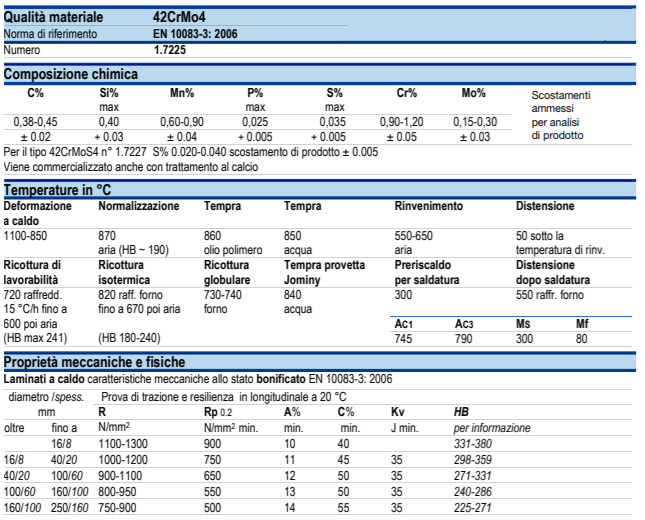
\includegraphics{Immagini/MaterialeAlberi.png}
    \caption{Propietà dell'acciaio 42CrMo4}
    \label{fig:MaterialeAlberi}
\end{figure}

Gli alberi sono stati interamente progettati attraverso il software KissSoft.
\newpage
\subsection{Metodologia applicata per la progettazione degli alberi mediante software}
All'interno del software è presente una sezione appositamente dedicata alla progettazione degli alberi chiamata "Alberi e cuscinetti".\\
\\
In primo luogo è necessario effettuare un disegno di massima dell'albero, compreso delle grandezze fondamentali come lunghezza e diametri, insieme a grandezze più di dettaglio come raggi di raccordo o gole di scarico. 
\begin{figure}[h]
    \centering
    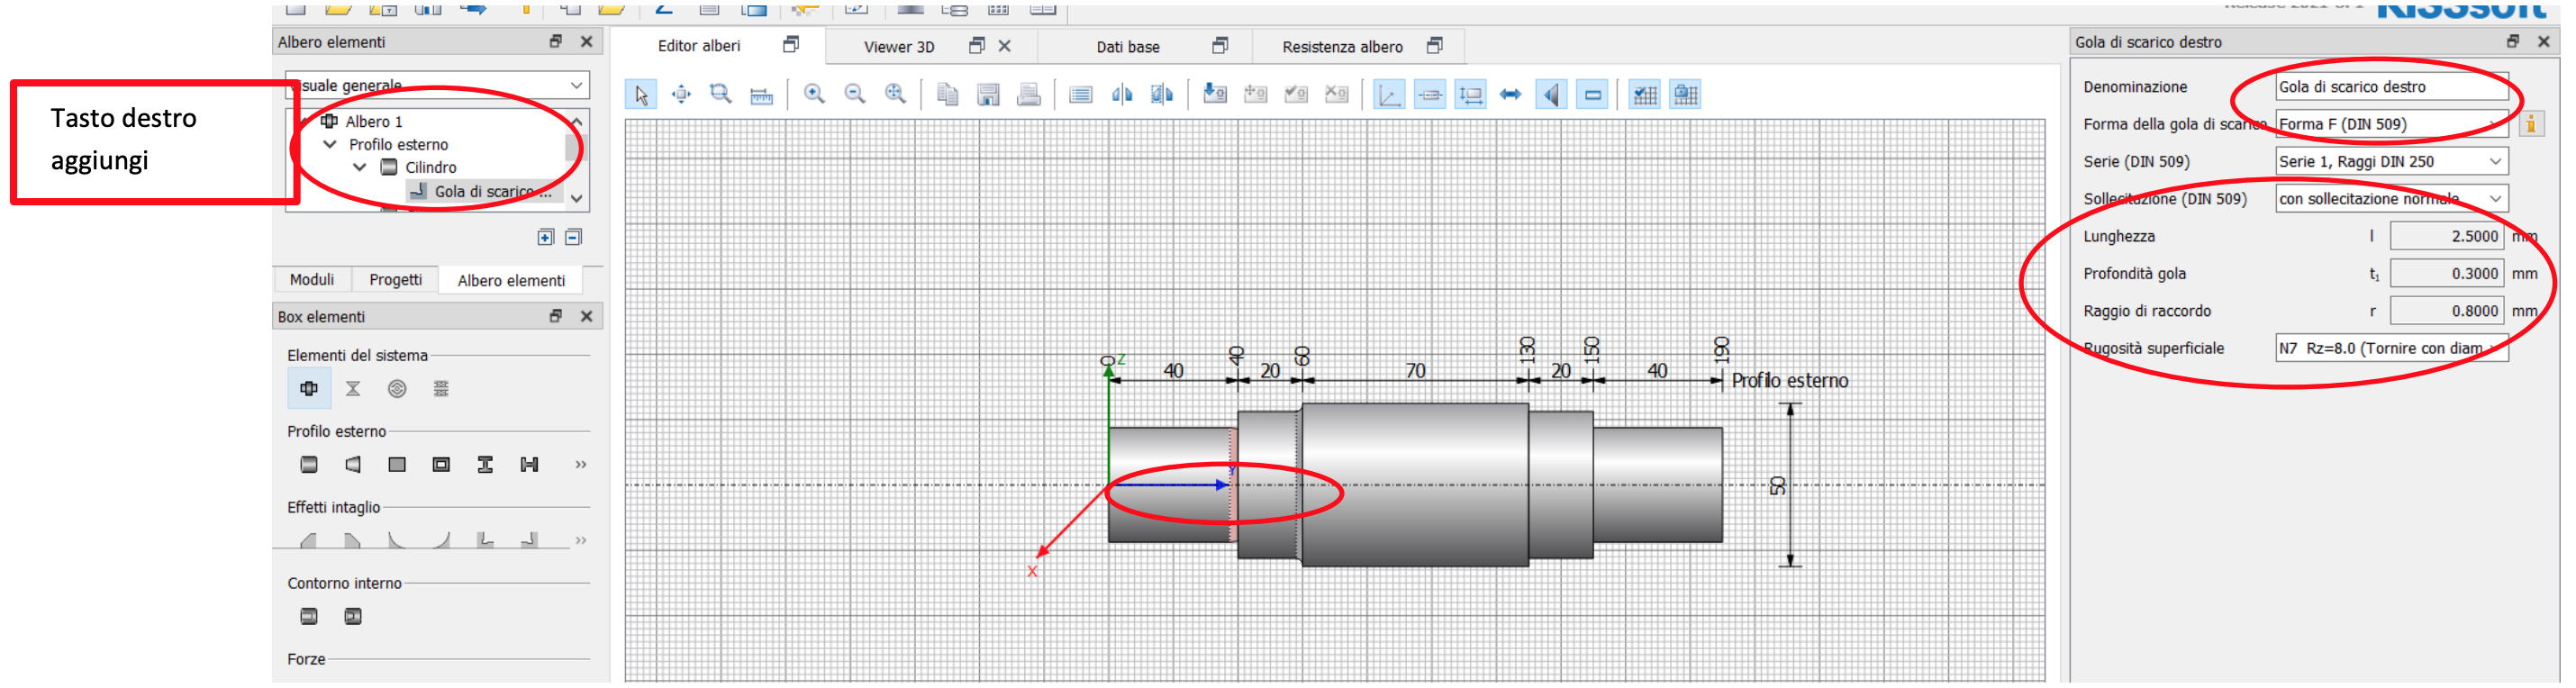
\includegraphics[scale=0.29]{Immagini/MetodologiaAlberi.png}
    \caption{Disegno di massima dell'albero}
    \label{fig:MetodologiaAlberi}
\end{figure}

In corrispondenza di zone di interesse come ad esempio spallamenti, gole di scarico ed intagli sono state aggiunte sezioni attraverso le quali è stato possibile eseguire l'analisi a fatica della stessa. 

Per eseguire l'analisi a fatica di un albero risulta necessario fornire al software il carico associato attraverso la definizione di cuscinetti, input di coppia ed output di coppia.\\
L'input di coppia corrisponde ad un ingranaggio calettato sull'albero, compreso del proprio ciclo di carico definito durante la sua progettazione (Fig.\ref{fig:MetodologiaAlberi2}).
\begin{figure}[h]
    \centering
    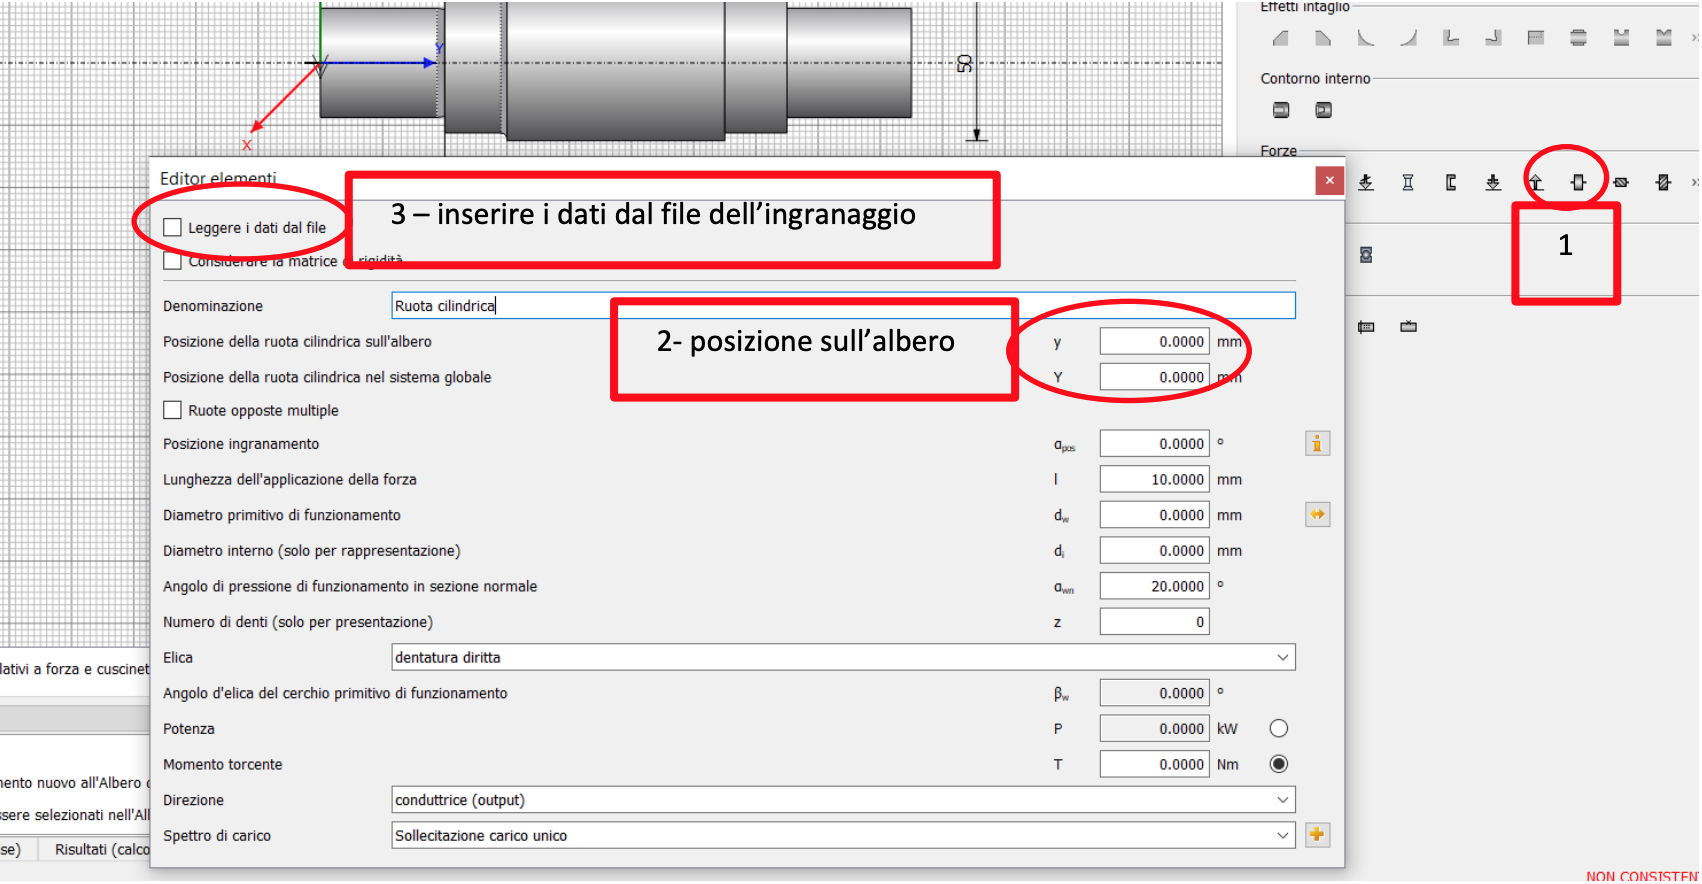
\includegraphics[scale=0.5]{Immagini/MetodologiaAlberi2.png}
    \caption{Inserimento dell'input di coppia sull'albero}
    \label{fig:MetodologiaAlberi2}
\end{figure}

La coppia che entra lungo l'albero deve anche uscire attraverso un altro ingranaggio oppure attraverso un elemento chiamato accoppiamento motore.

Definiti questi parametri, sarà necessario esplicitare i vincoli dell'albero attraverso la scelta e il bloccaggio dei cuscinetti.
\begin{figure}[h]
    \centering
    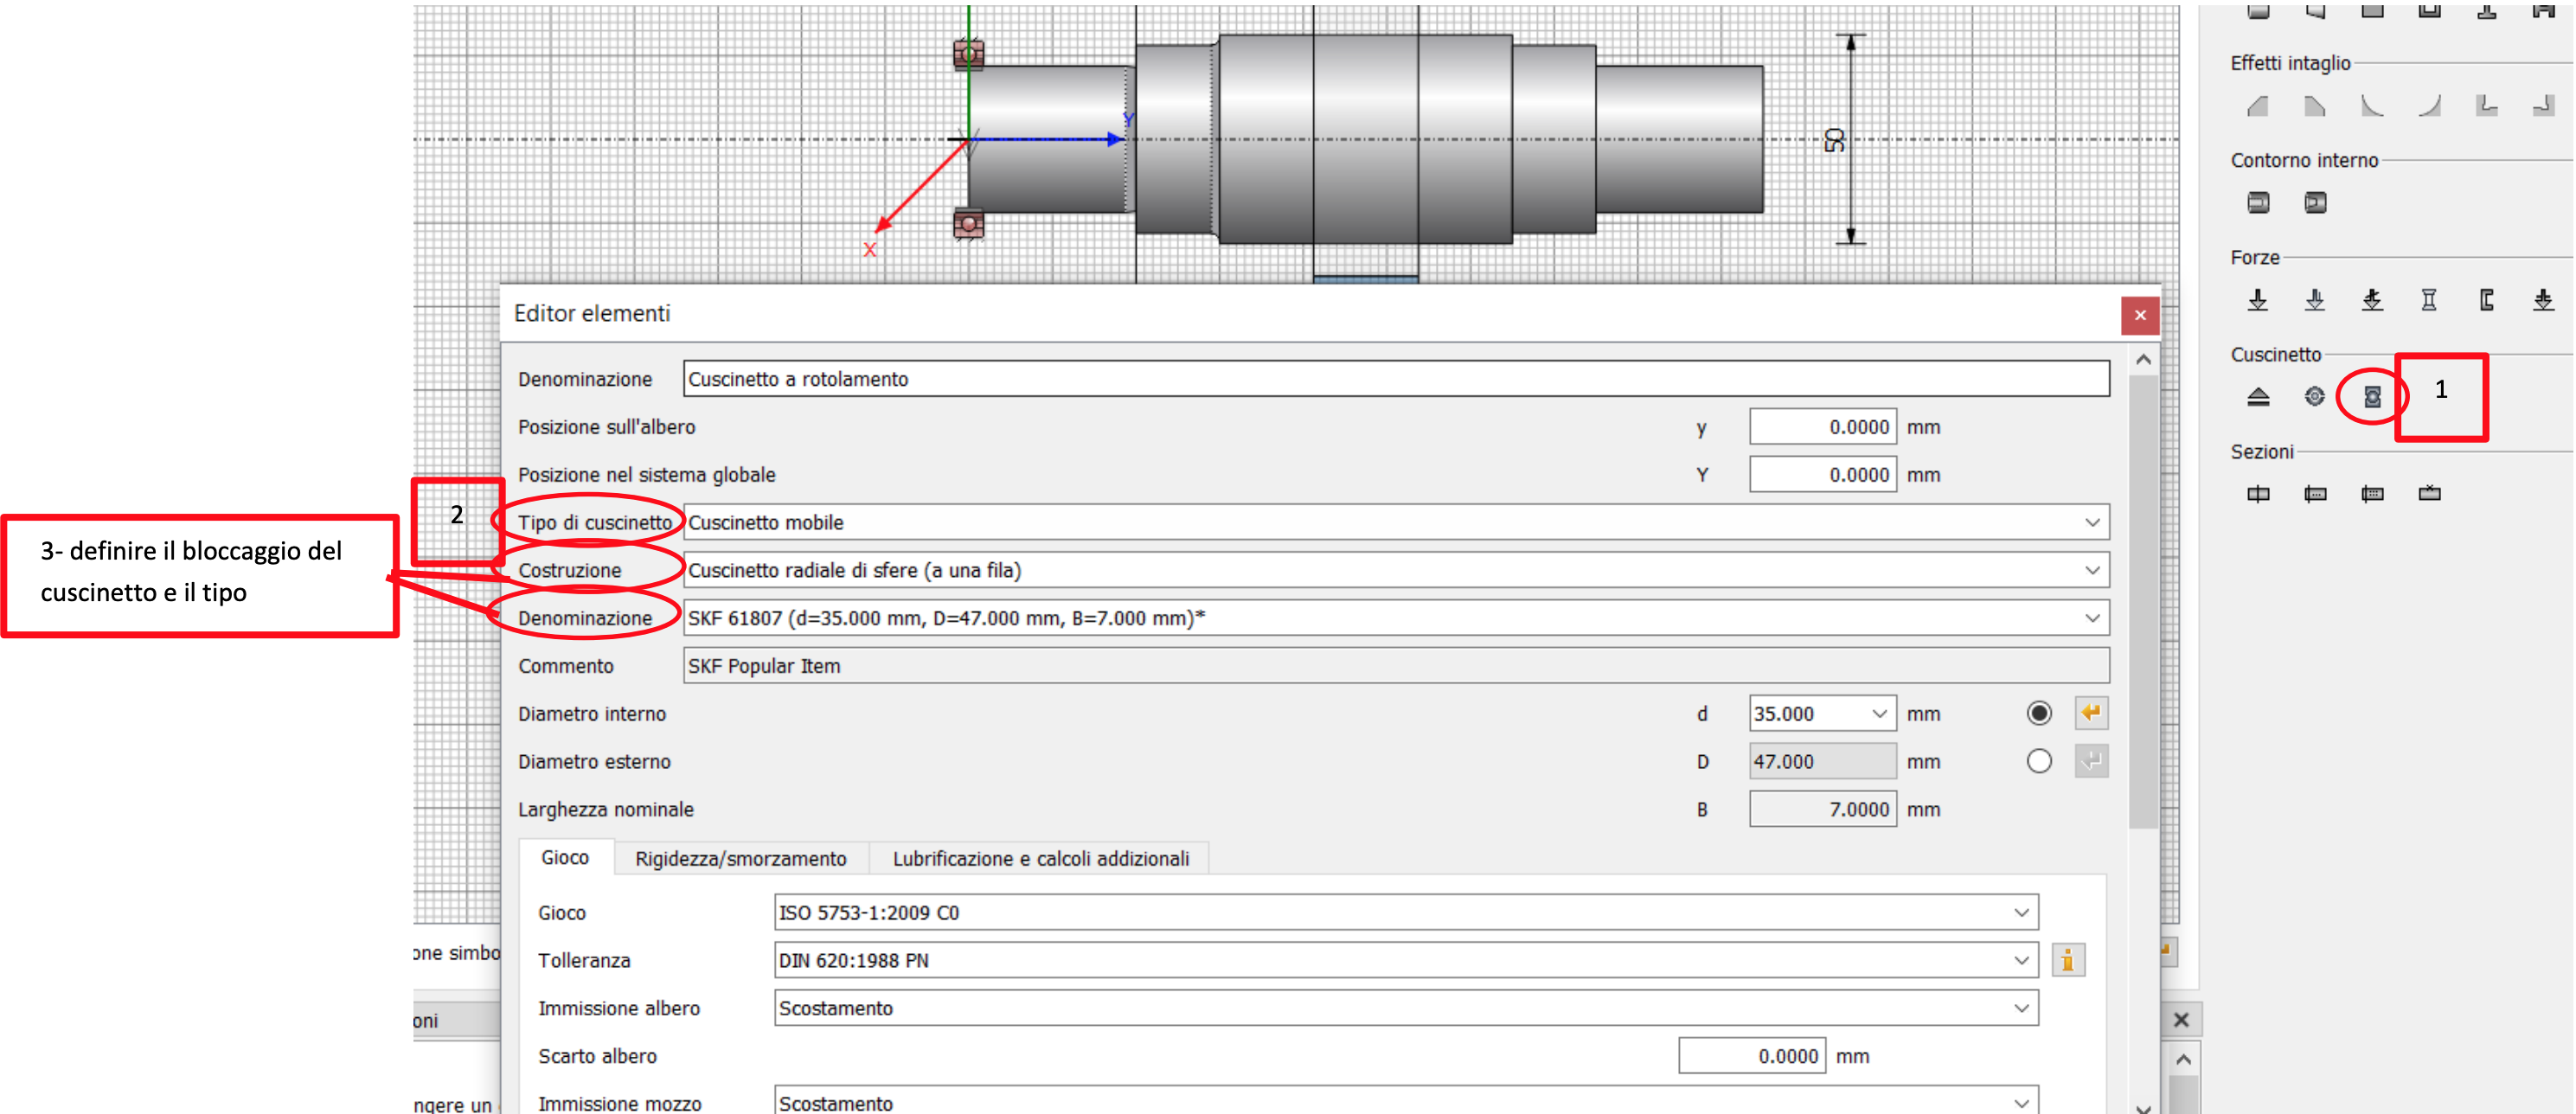
\includegraphics[scale=0.27]{Immagini/MetodologiaAlberi3.png}
    \caption{Scelta dei cuscinetti dell'albero}
    \label{fig:MetodologiaAlberi3}
\end{figure}

Terminato questo processo è sufficiente inserire il materiale di cui è costituito l'albero, considerare gli ingranaggi come massa e rigidezza e inserire il verso di rotazione trovato utilizzando la regola della mano destra, per eseguire l'analisi dell'elemento in questione. \begin{figure}[h]
    \centering
    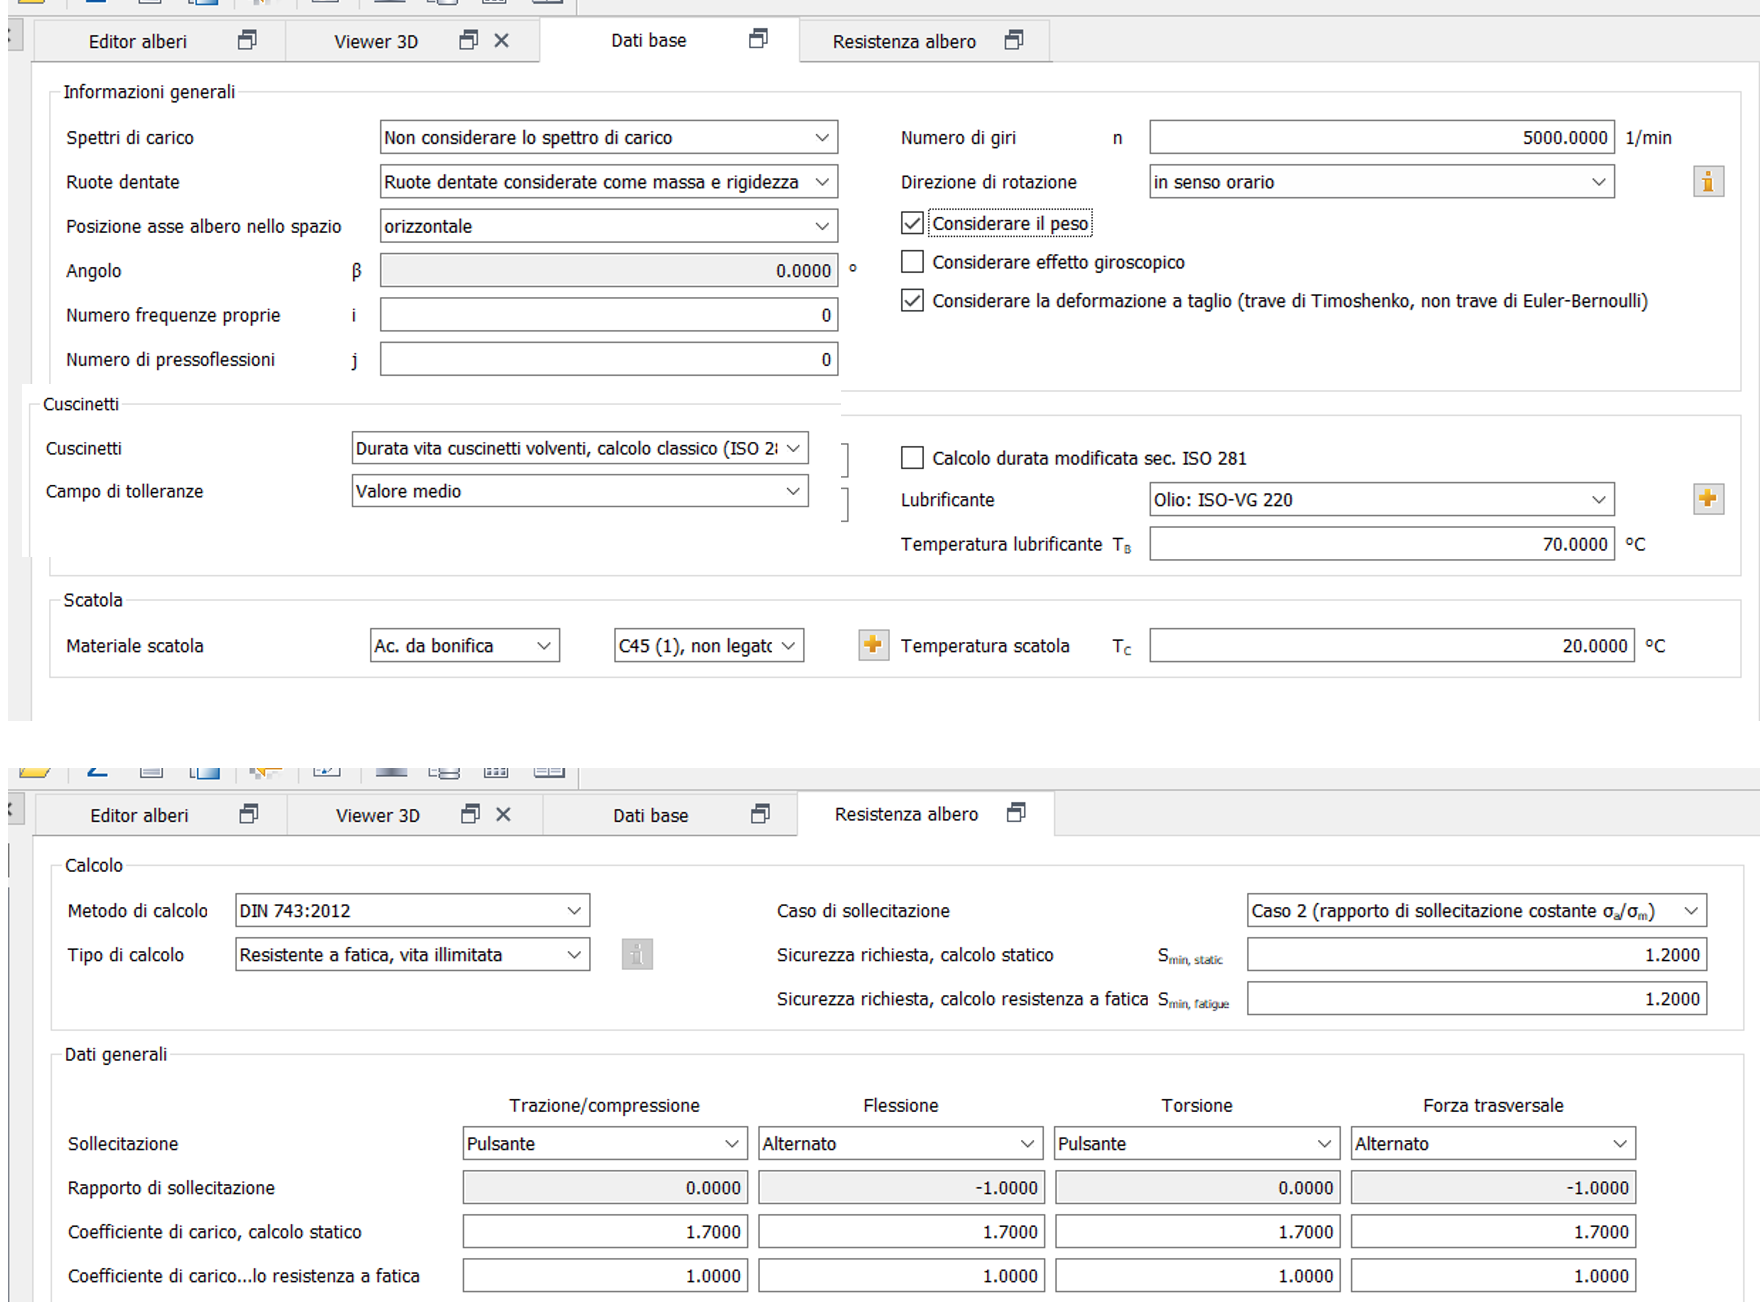
\includegraphics[scale=0.4]{Immagini/MetodologiaAlberi4.png}
    \caption{Inserimento di ultimi dettagli di interesse per l'analisi degli alberi mediante KissSoft}
    \label{fig:MetodologiaAlberi4}
\end{figure}

Questo processo è stato ripetuto per ogni albero del riduttore in esame.
\newpage
\paragraph{Albero 1}
L'albero 1 è l'albero in input al riduttore.
\begin{figure}[h]
    \centering
    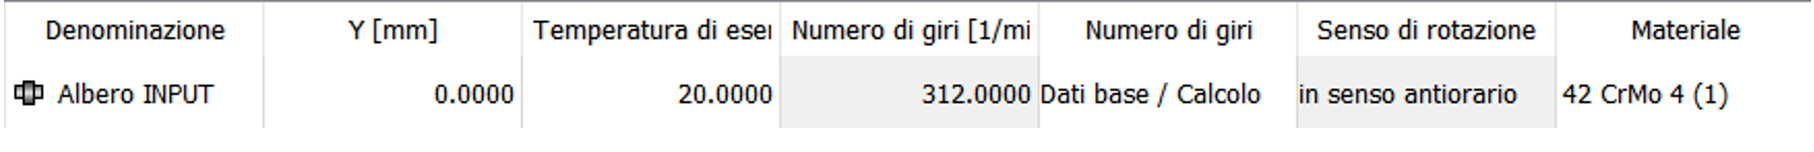
\includegraphics[scale=0.45]{Immagini/DatiAlbero1.png}
    \caption{Albero  1}
    \label{fig:DatiAlbero1}
\end{figure}

Sono state individuate sei sezioni di interesse:
\begin{itemize}
    \item Due sezioni per le gole di scarico (cuscinetto sinistra e destra);
    \item Tre sezioni per gli spallamenti;
    \item Una sezione per la sede dell'anello Seeger.
\end{itemize}
\newpage
\begin{figure}[h]
    \centering
    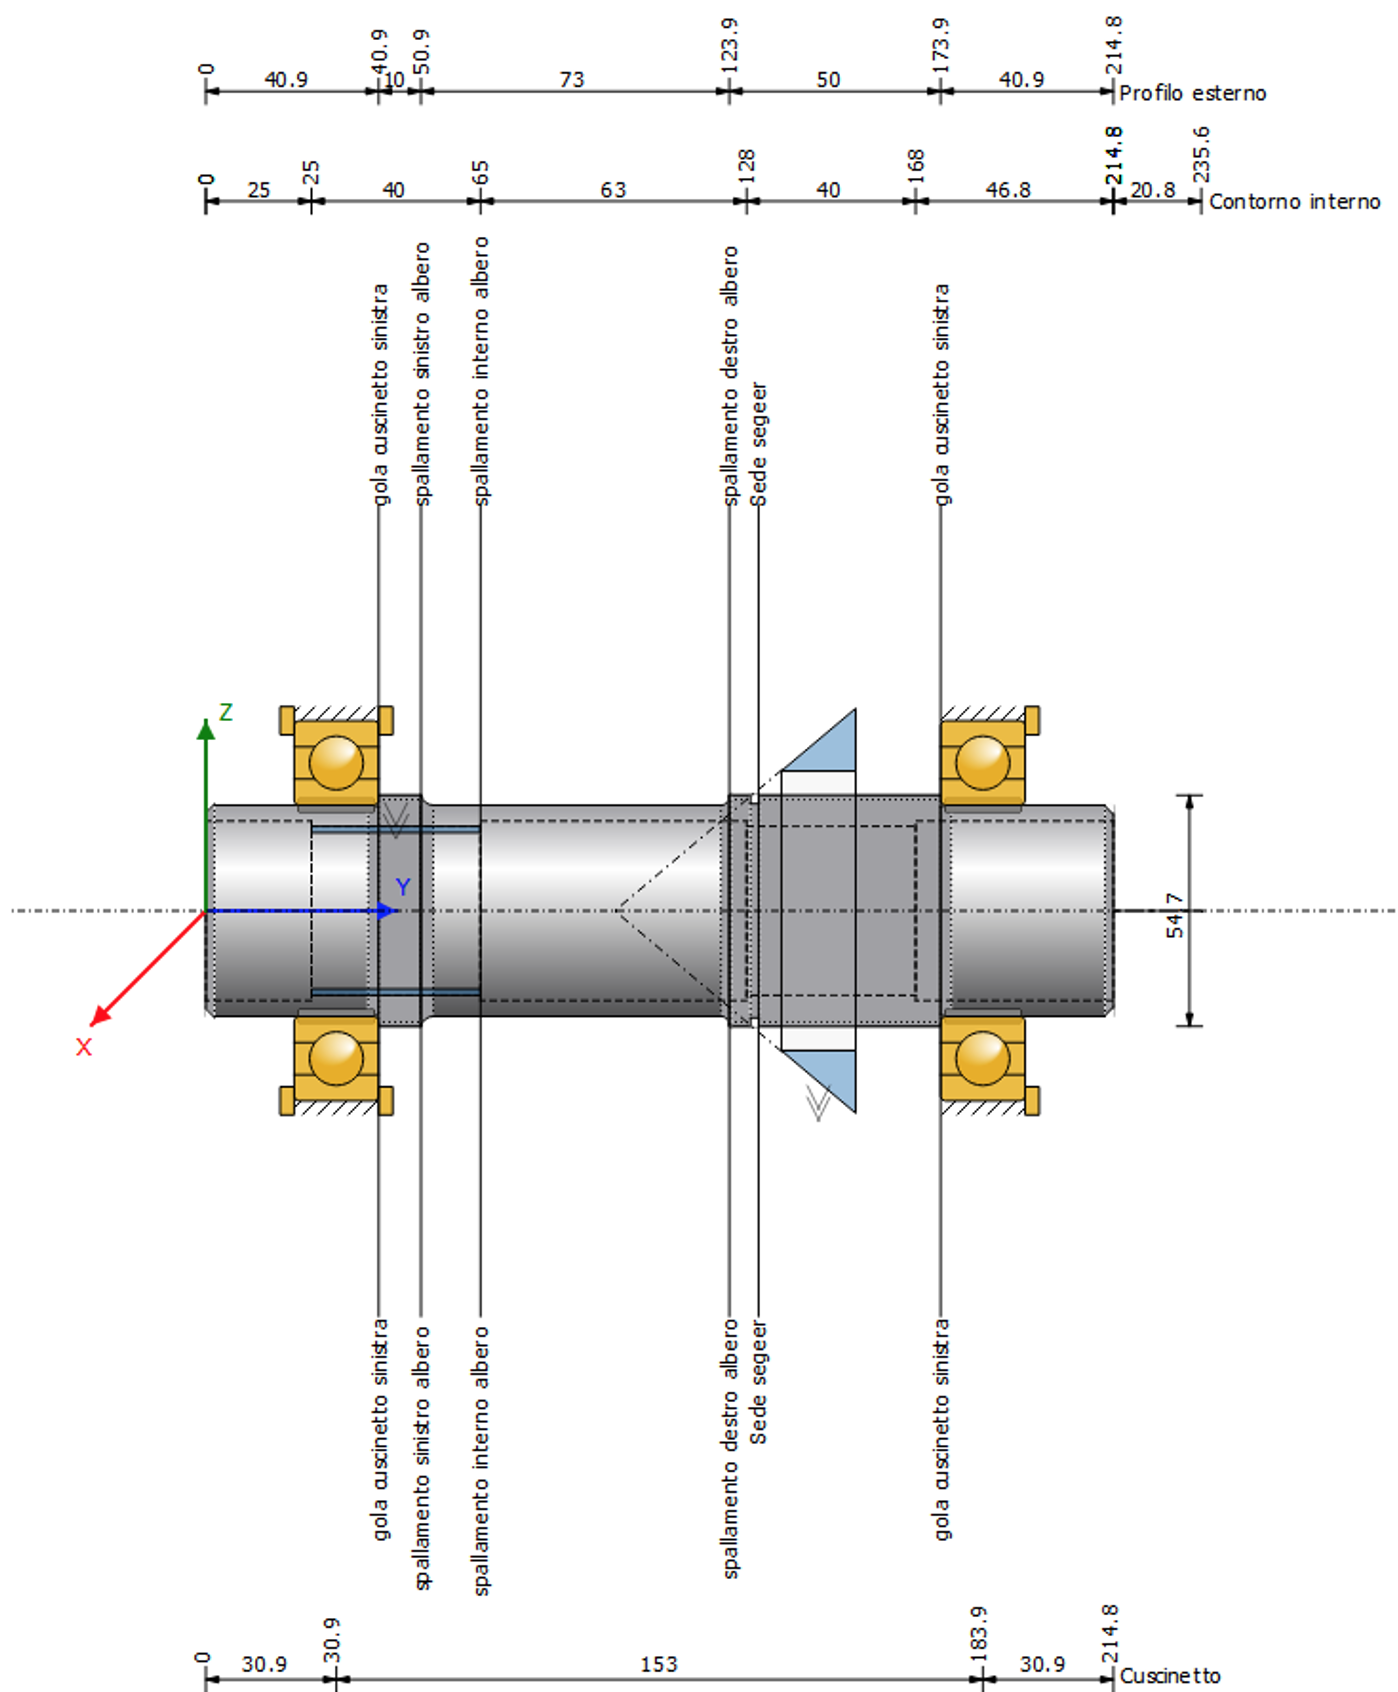
\includegraphics[scale=0.55]{Immagini/Albero1.png}
    \caption{Layout Albero 1}
    \label{fig:Albero1}
\end{figure}
\newpage

Il cuscinetto sinistro inserito possiede le seguenti caratteristiche
\begin{figure}[h]
    \centering
    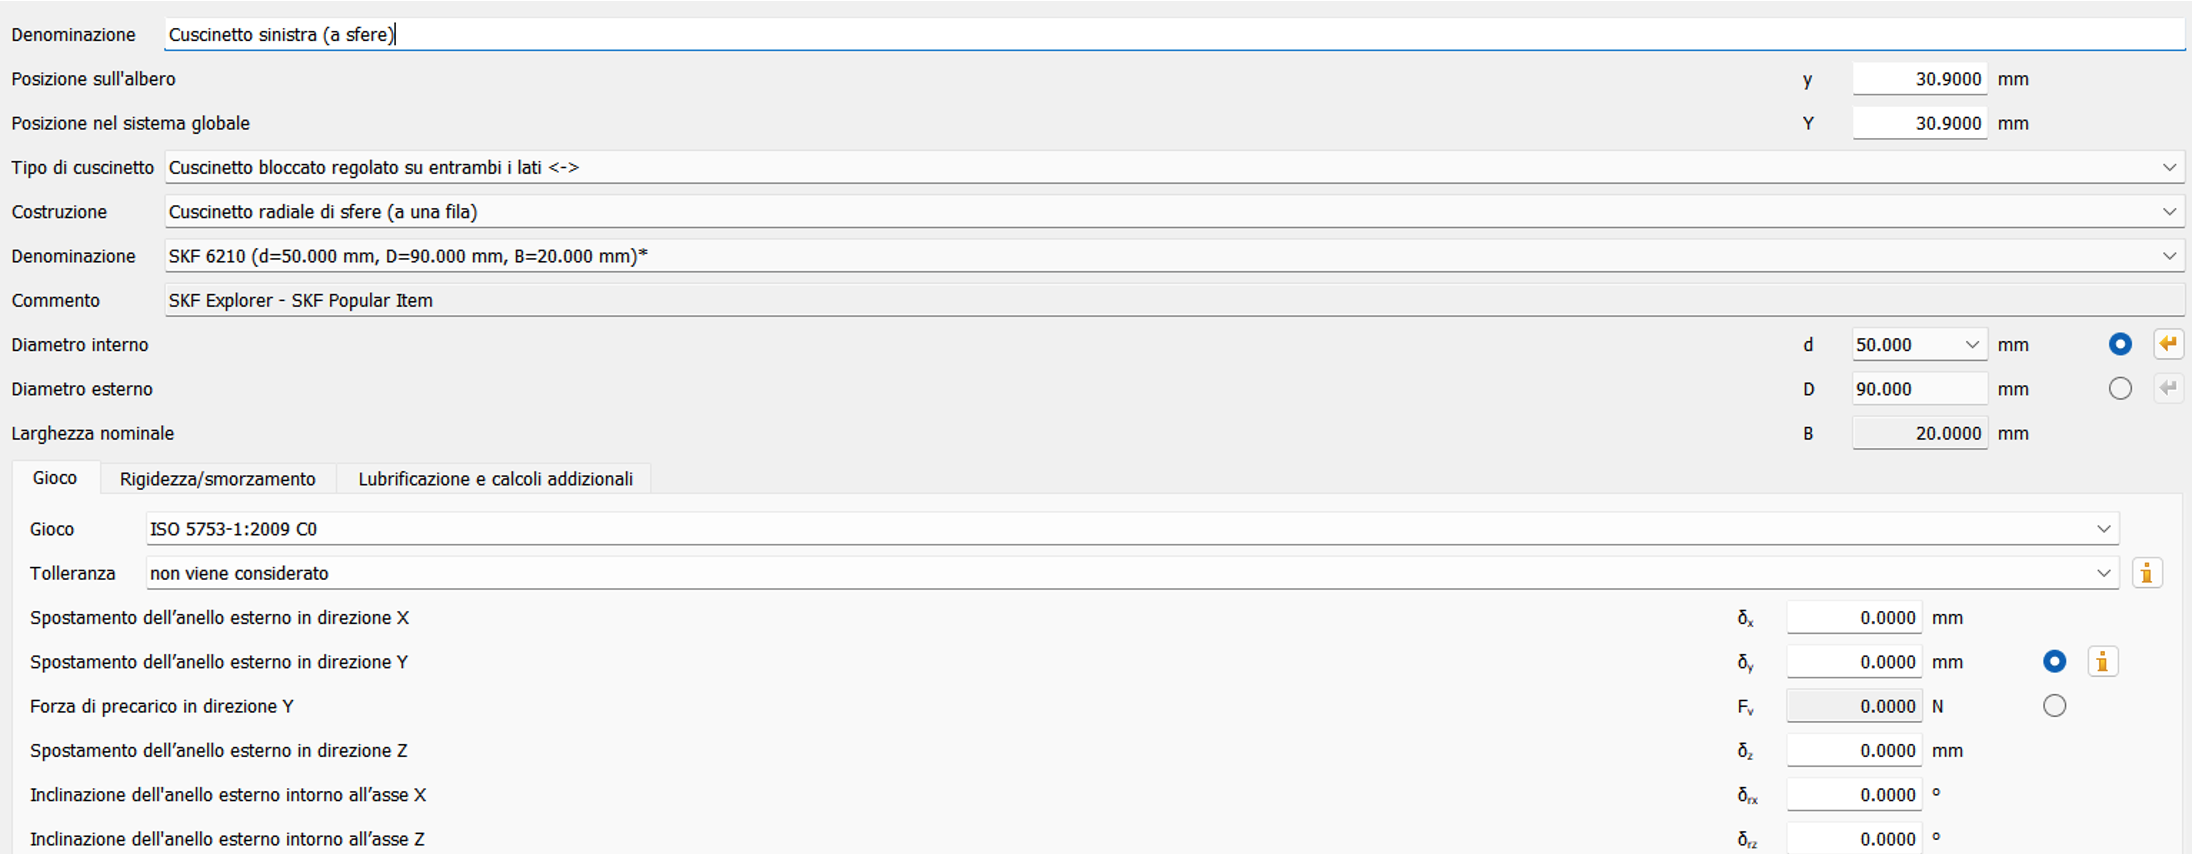
\includegraphics[scale=0.4]{Immagini/CuscinettoSinistraAlbero1.png}
    \caption{Caratteristiche cuscinetto sinistro relativo all'albero 1}
    \label{fig:CuscinettoSinsitraAlbero1}
\end{figure}

mentre il cuscinetto destro
\begin{figure}[h]
    \centering
    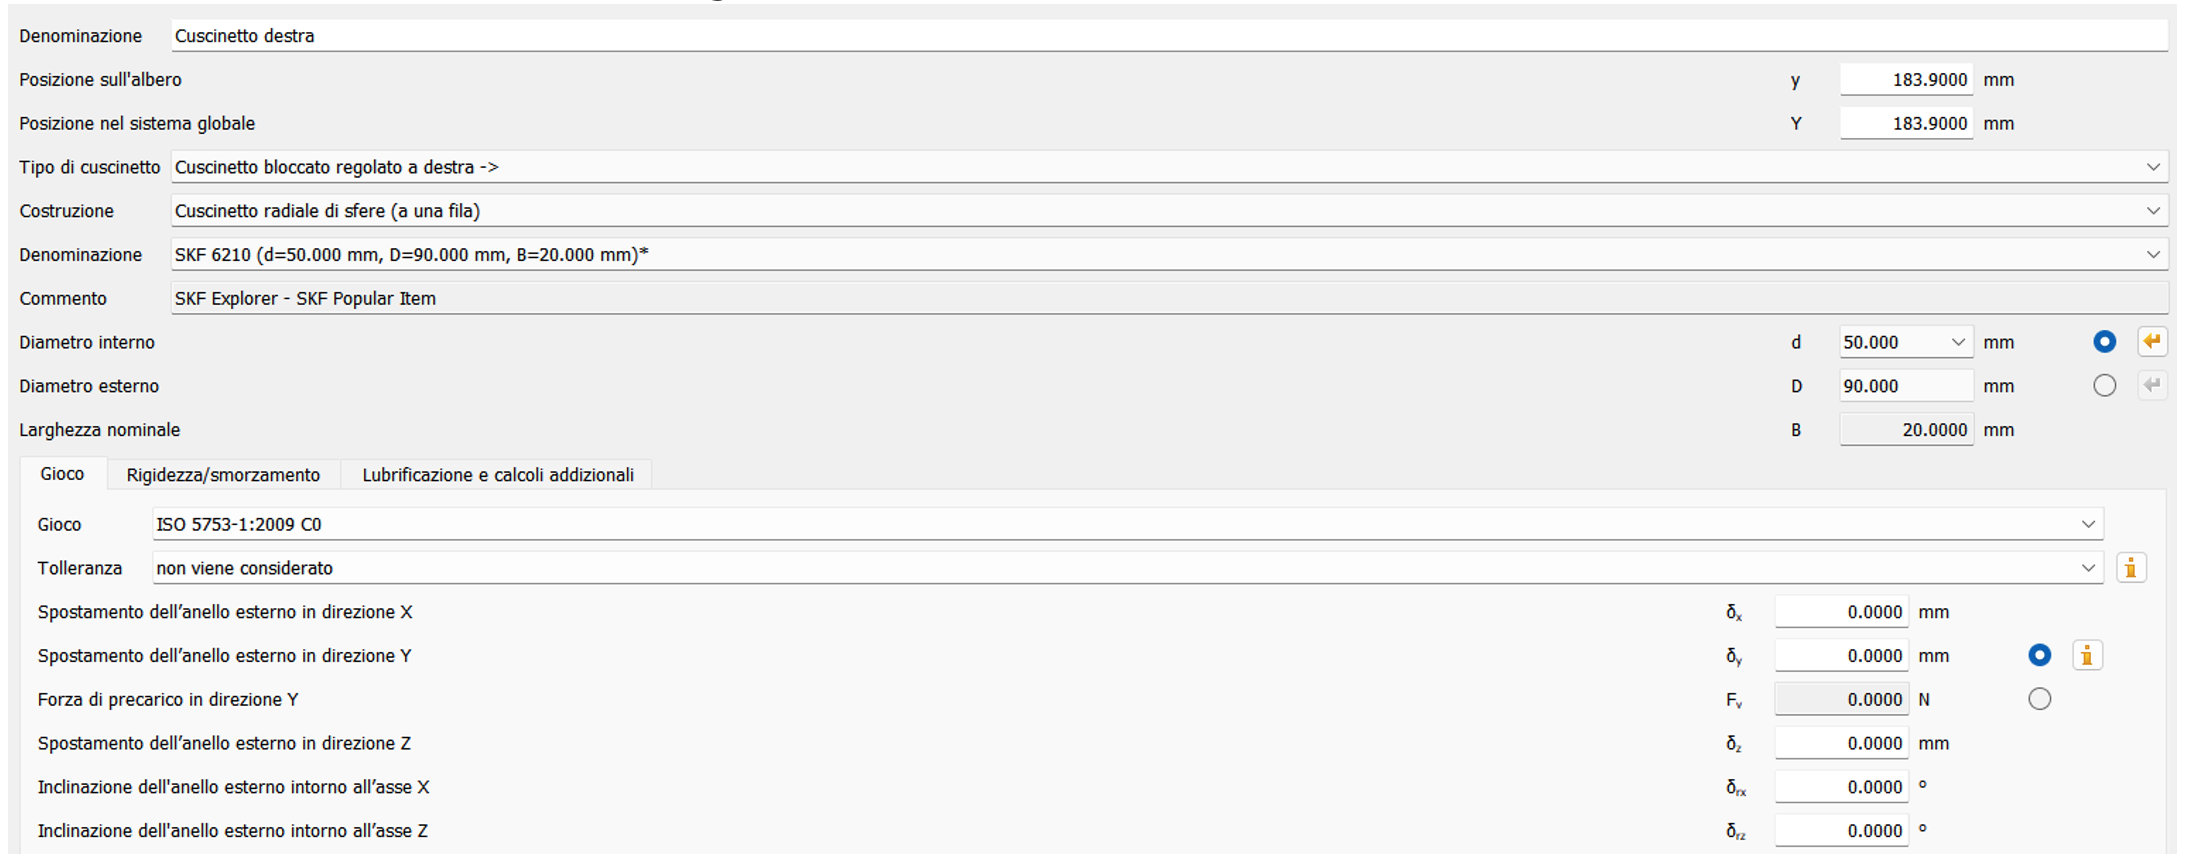
\includegraphics[scale=0.4]{Immagini/CuscinettoDestraAlbero1.png}
    \caption{Caratteristiche cuscinetto destro relativo all'albero 1}
    \label{fig:CuscinettoDestraAlbero1}
\end{figure}
\newpage
La ruota conica montata sull'albero corrisponde alla ruota 0 precedentemente dimensionata, ed è la ruota da cui esce la coppia. Le caratteristiche di questa ruota sono riportate di seguito.
\begin{figure}[h]
    \centering
    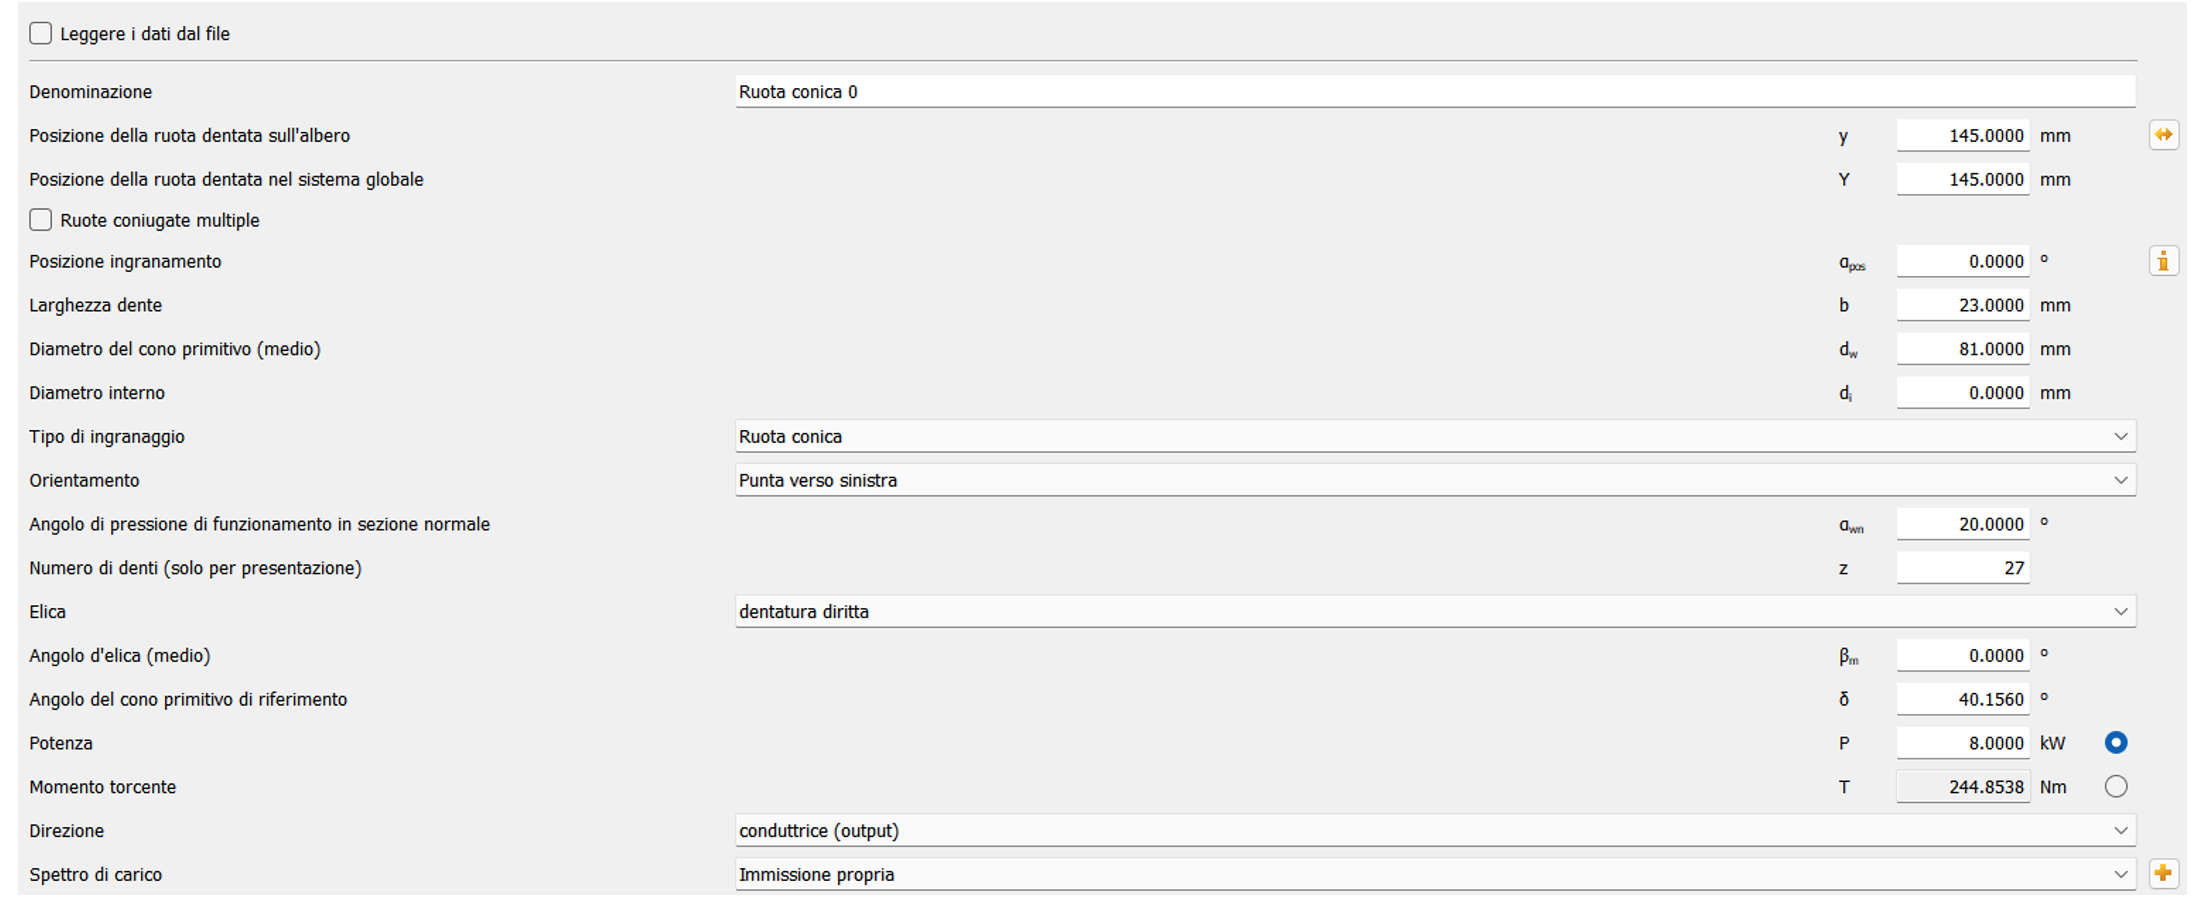
\includegraphics[scale=0.4]{Immagini/Ruota0Albero1.png}
    \caption{Dati della ruota 0 calettata sull'albero 1}
    \label{fig:Ruota0Albero1}
\end{figure}

È stato necessario considerare il momento torcente in ingresso dato dall'accoppiamento motore secondo i seguenti parametri.
\begin{figure}[h]
    \centering
    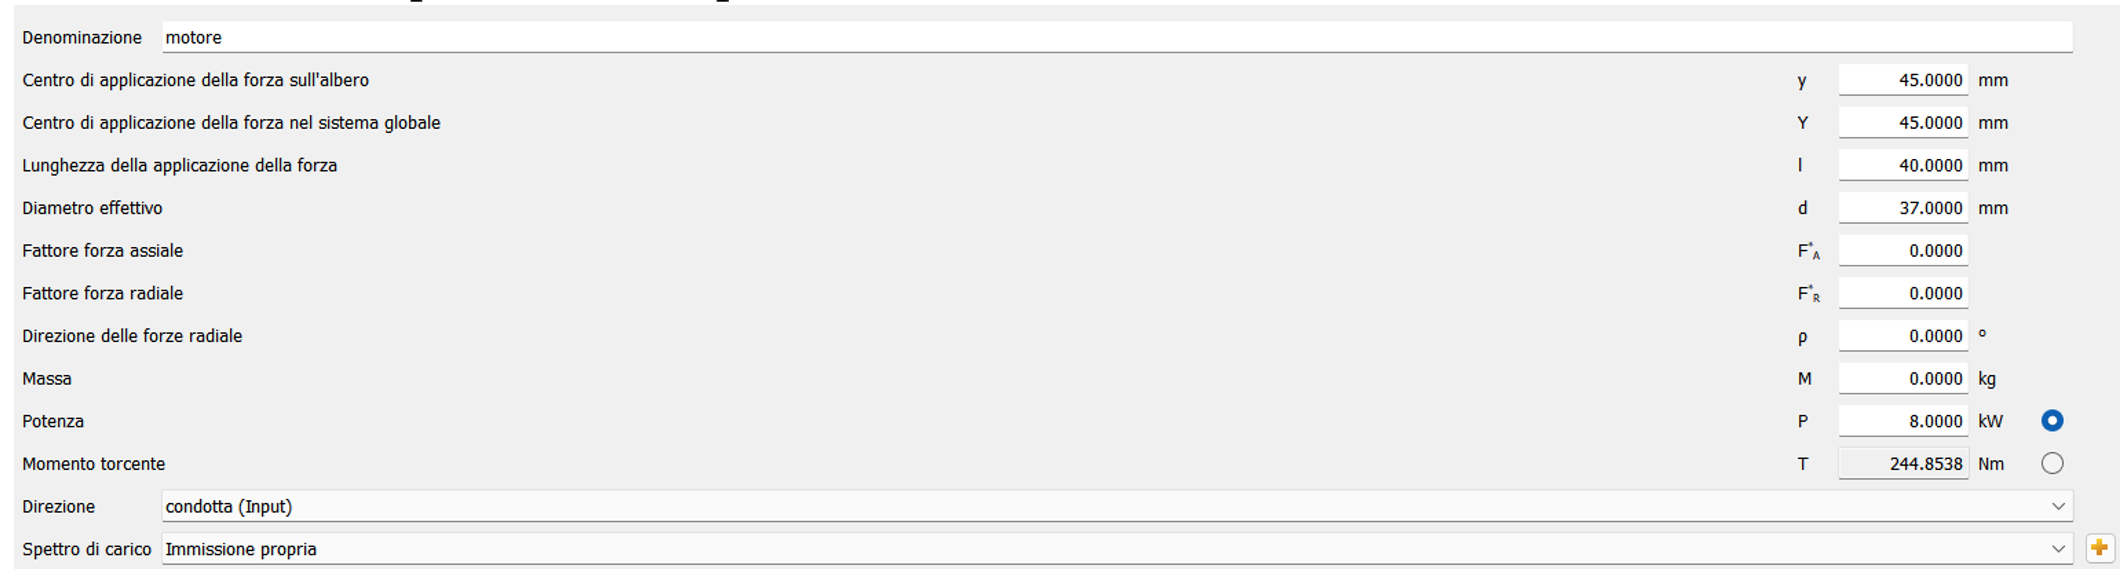
\includegraphics[scale=0.4]{Immagini/MomentoAlbero1.png}
    \caption{Momento torcente in ingresso all'albero 1}
    \label{fig:MomentoAlbero1}
\end{figure}
\newpage
Sono state poi considerate le grandezze di dettaglio:
\begin{figure}[h]
    \centering
    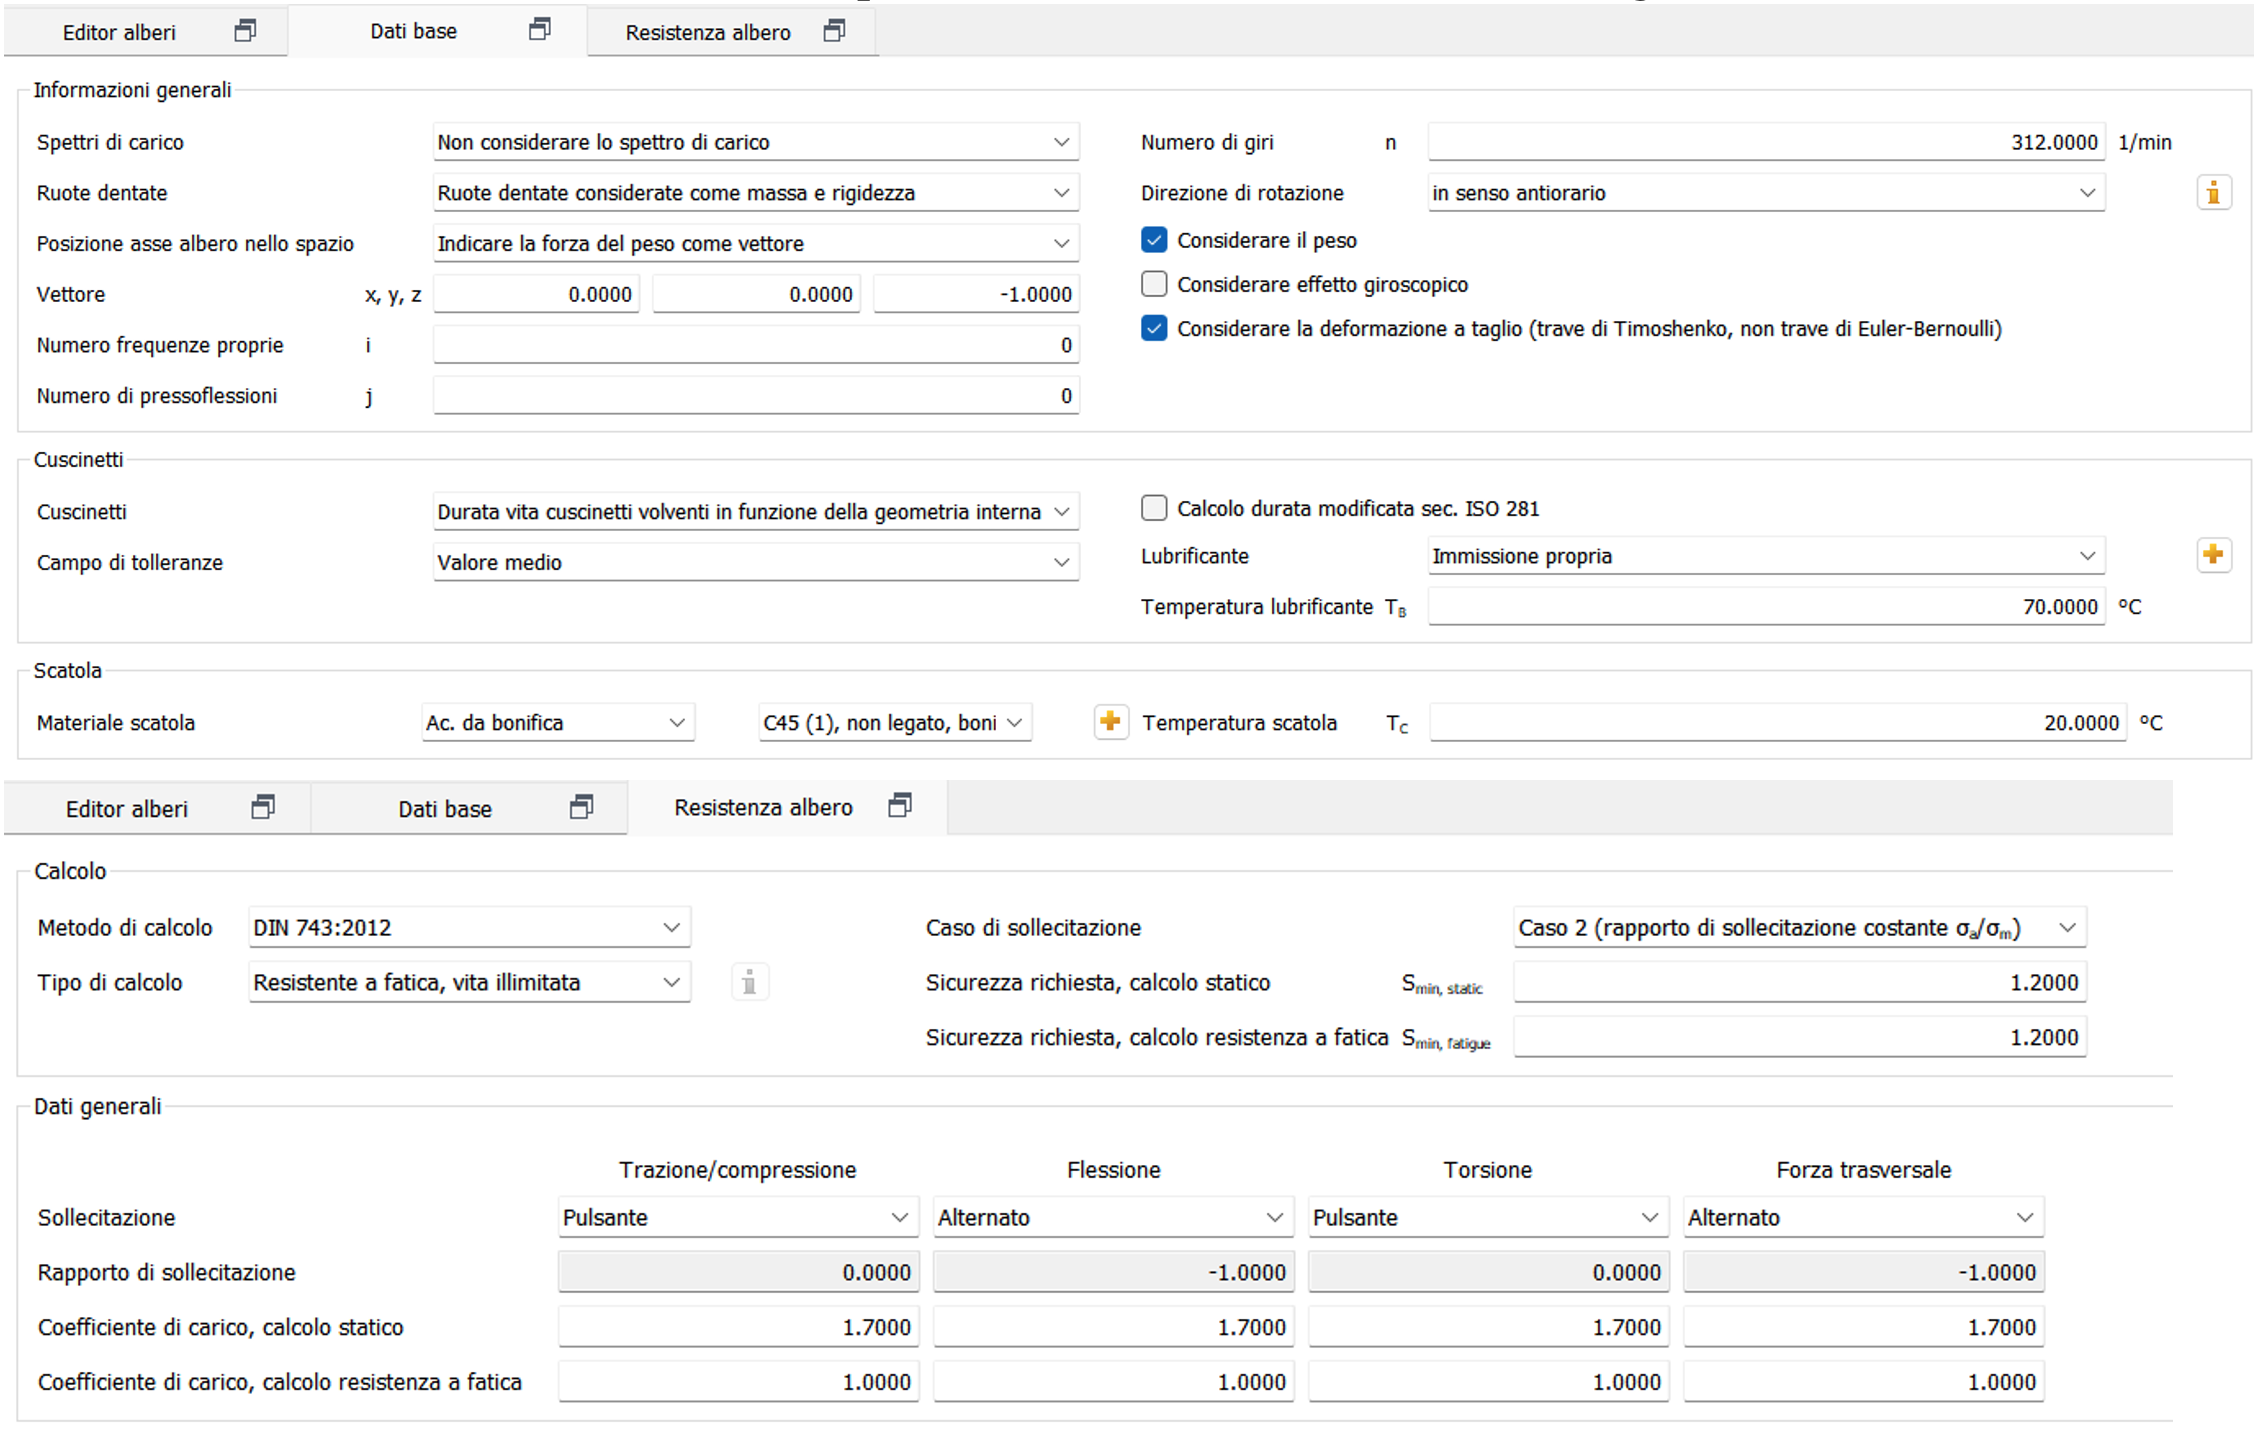
\includegraphics[scale=0.4]{Immagini/DettagliAlbero1.png}
    \caption{Grandezze di dettaglio relative all'analisi dell'albero 1}
    \label{fig:DettagliAlbero1}
\end{figure}

Dal Report fornito dal software è possibile ottenere ulteriori informazioni di interesse sull'albero appena progettato. 

\emph{Applicazione del carico}
\begin{figure}[h]
    \centering
    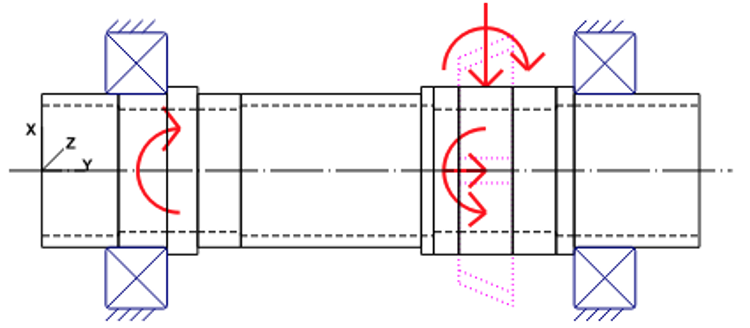
\includegraphics[scale=0.5]{Immagini/CaricoAlbero1.png}
    \caption{Applicazione del carico lungo l'albero 1}
    \label{fig:CaricoAlbero1}
\end{figure}
\newpage
\emph{Forze agenti sulle ruote}
\begin{figure}[h]
    \centering
    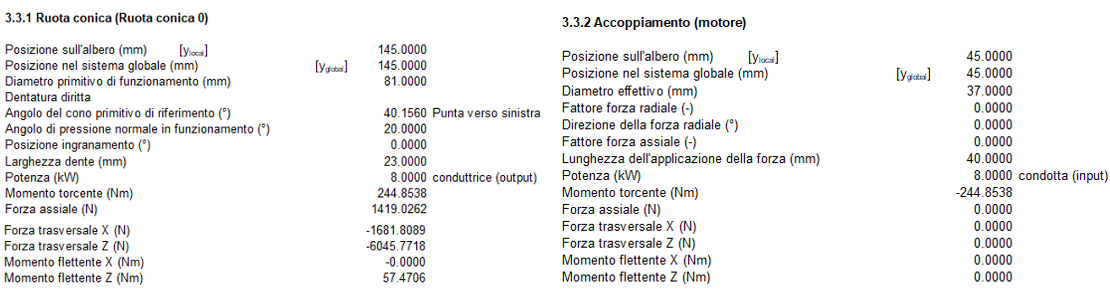
\includegraphics[scale=0.7]{Immagini/ForzeRuoteAlbero1.png}
    \caption{Valore delle forze trasmesse sull'albero 1}
    \label{fig:ForzeRuoteAlbero1}
\end{figure}

\emph{Dettagli cuscinetti}
\begin{figure}[h]
    \centering
    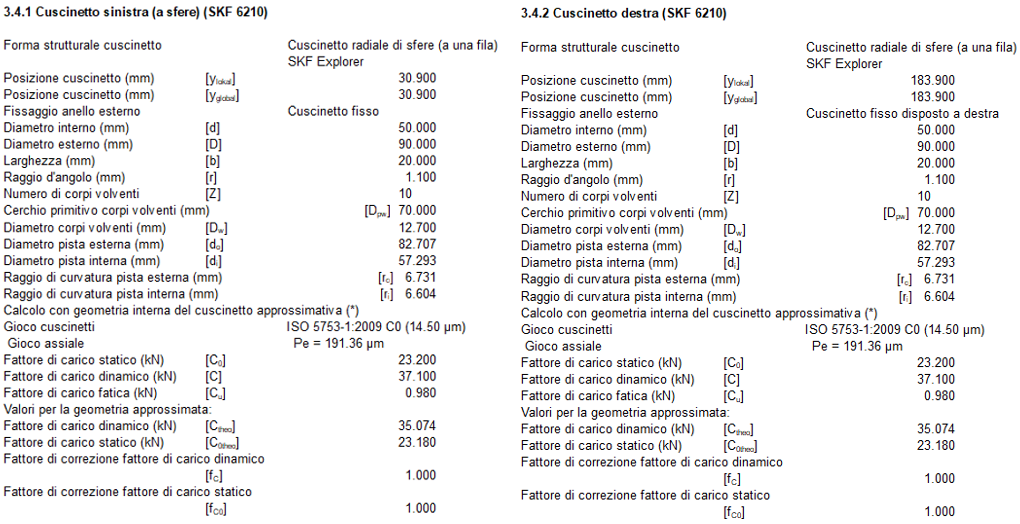
\includegraphics[scale=0.7]{Immagini/ForzeCuscinettiAlbero1.png}
    \caption{Valore delle forze trasmesse sull'albero 1}
    \label{fig:ForzeCusinettiAlbero1}
\end{figure}
\newpage
\emph{Deformazione dell'albero}
\begin{figure}[h]
    \centering
    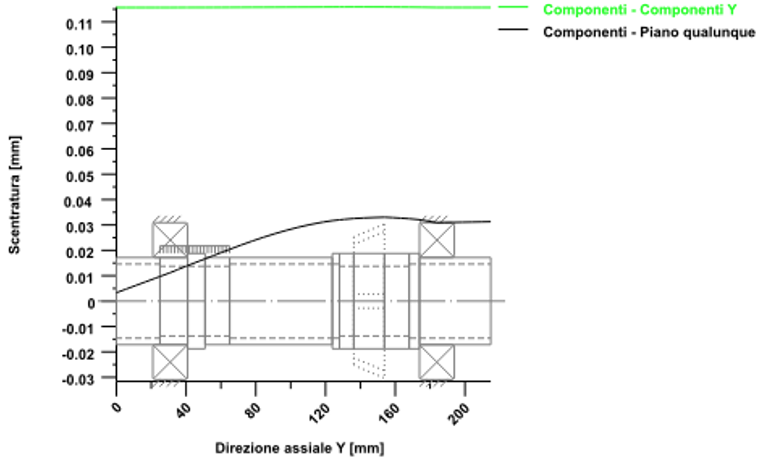
\includegraphics[scale=0.6]{Immagini/DeformataAlbero1.png}
    \caption{Deformata dell'albero 1}
    \label{fig:Deformata albero 1}
\end{figure}


\emph{Andamento della tensione equivalente}
\begin{figure}[h]
    \centering
    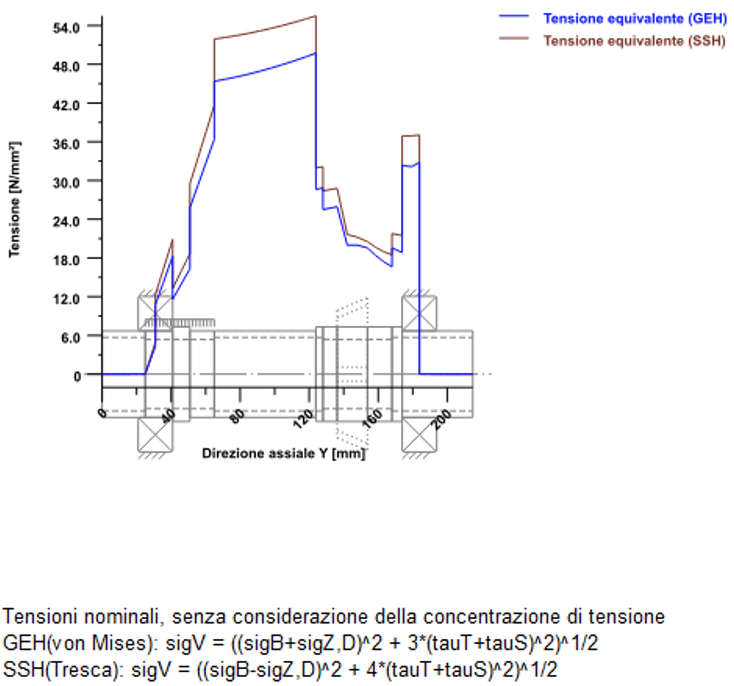
\includegraphics[scale=0.6]{Immagini/TensioniAlbero1.png}
    \caption{Andamento della tensione equivalente lungo l'albero 1}
    \label{fig:TensioniAlbero1}
\end{figure}
\newpage
Infine, attraverso la compilazione del software si è osservato come tutte le sezioni fossero ampiamente verificate sia staticamente che a fatica.
\begin{figure}[h]
    \centering
    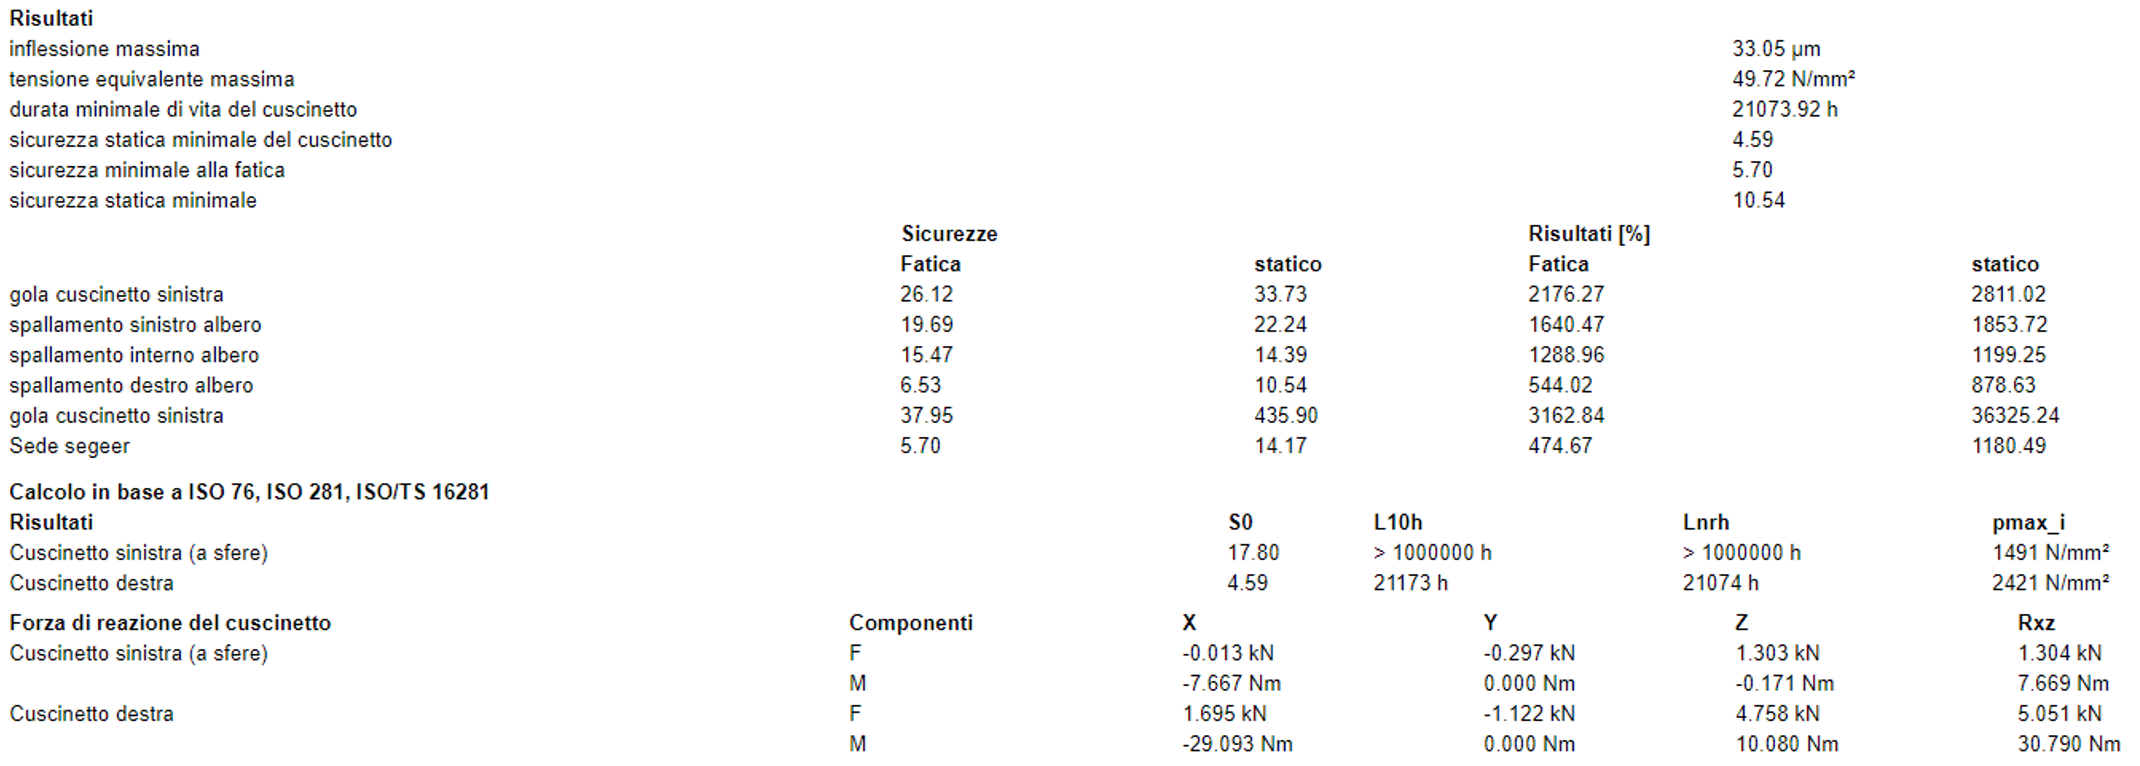
\includegraphics[scale=0.4]{Immagini/RisultatiAlbero1.png}
    \caption{Risultato dell'analisi statica e a fatica delle sezioni di interesse dell'albero 1}
    \label{fig:RisultatiALbero1}
\end{figure}

\paragraph{Albero 2}
Sono state individuate tre sezioni di interesse:
\begin{itemize}
    \item Una sezione sulla sede del cuscinetto a sinistra;
    \item Due sezioni per inizio e fine del profilo scanalato;
\end{itemize}

\begin{figure}[h]
    \centering
    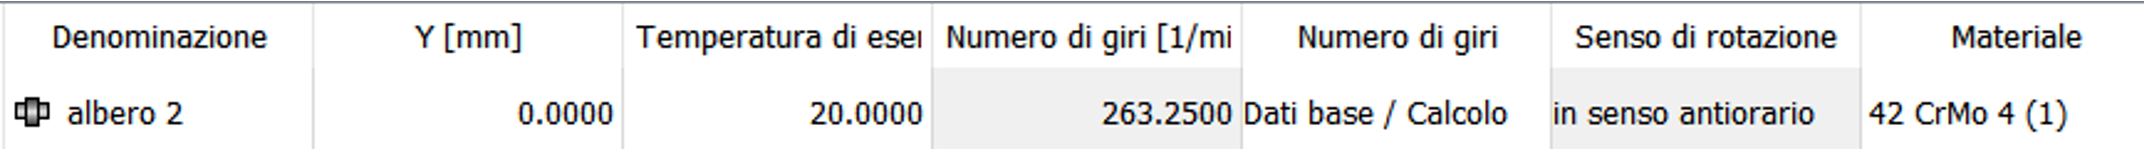
\includegraphics[scale=0.4]{Immagini/DatiAlbero2.png}
    \caption{Albero  2}
    \label{fig:DatiAlbero2}
\end{figure}
\newpage
\begin{figure}[h]
    \centering
    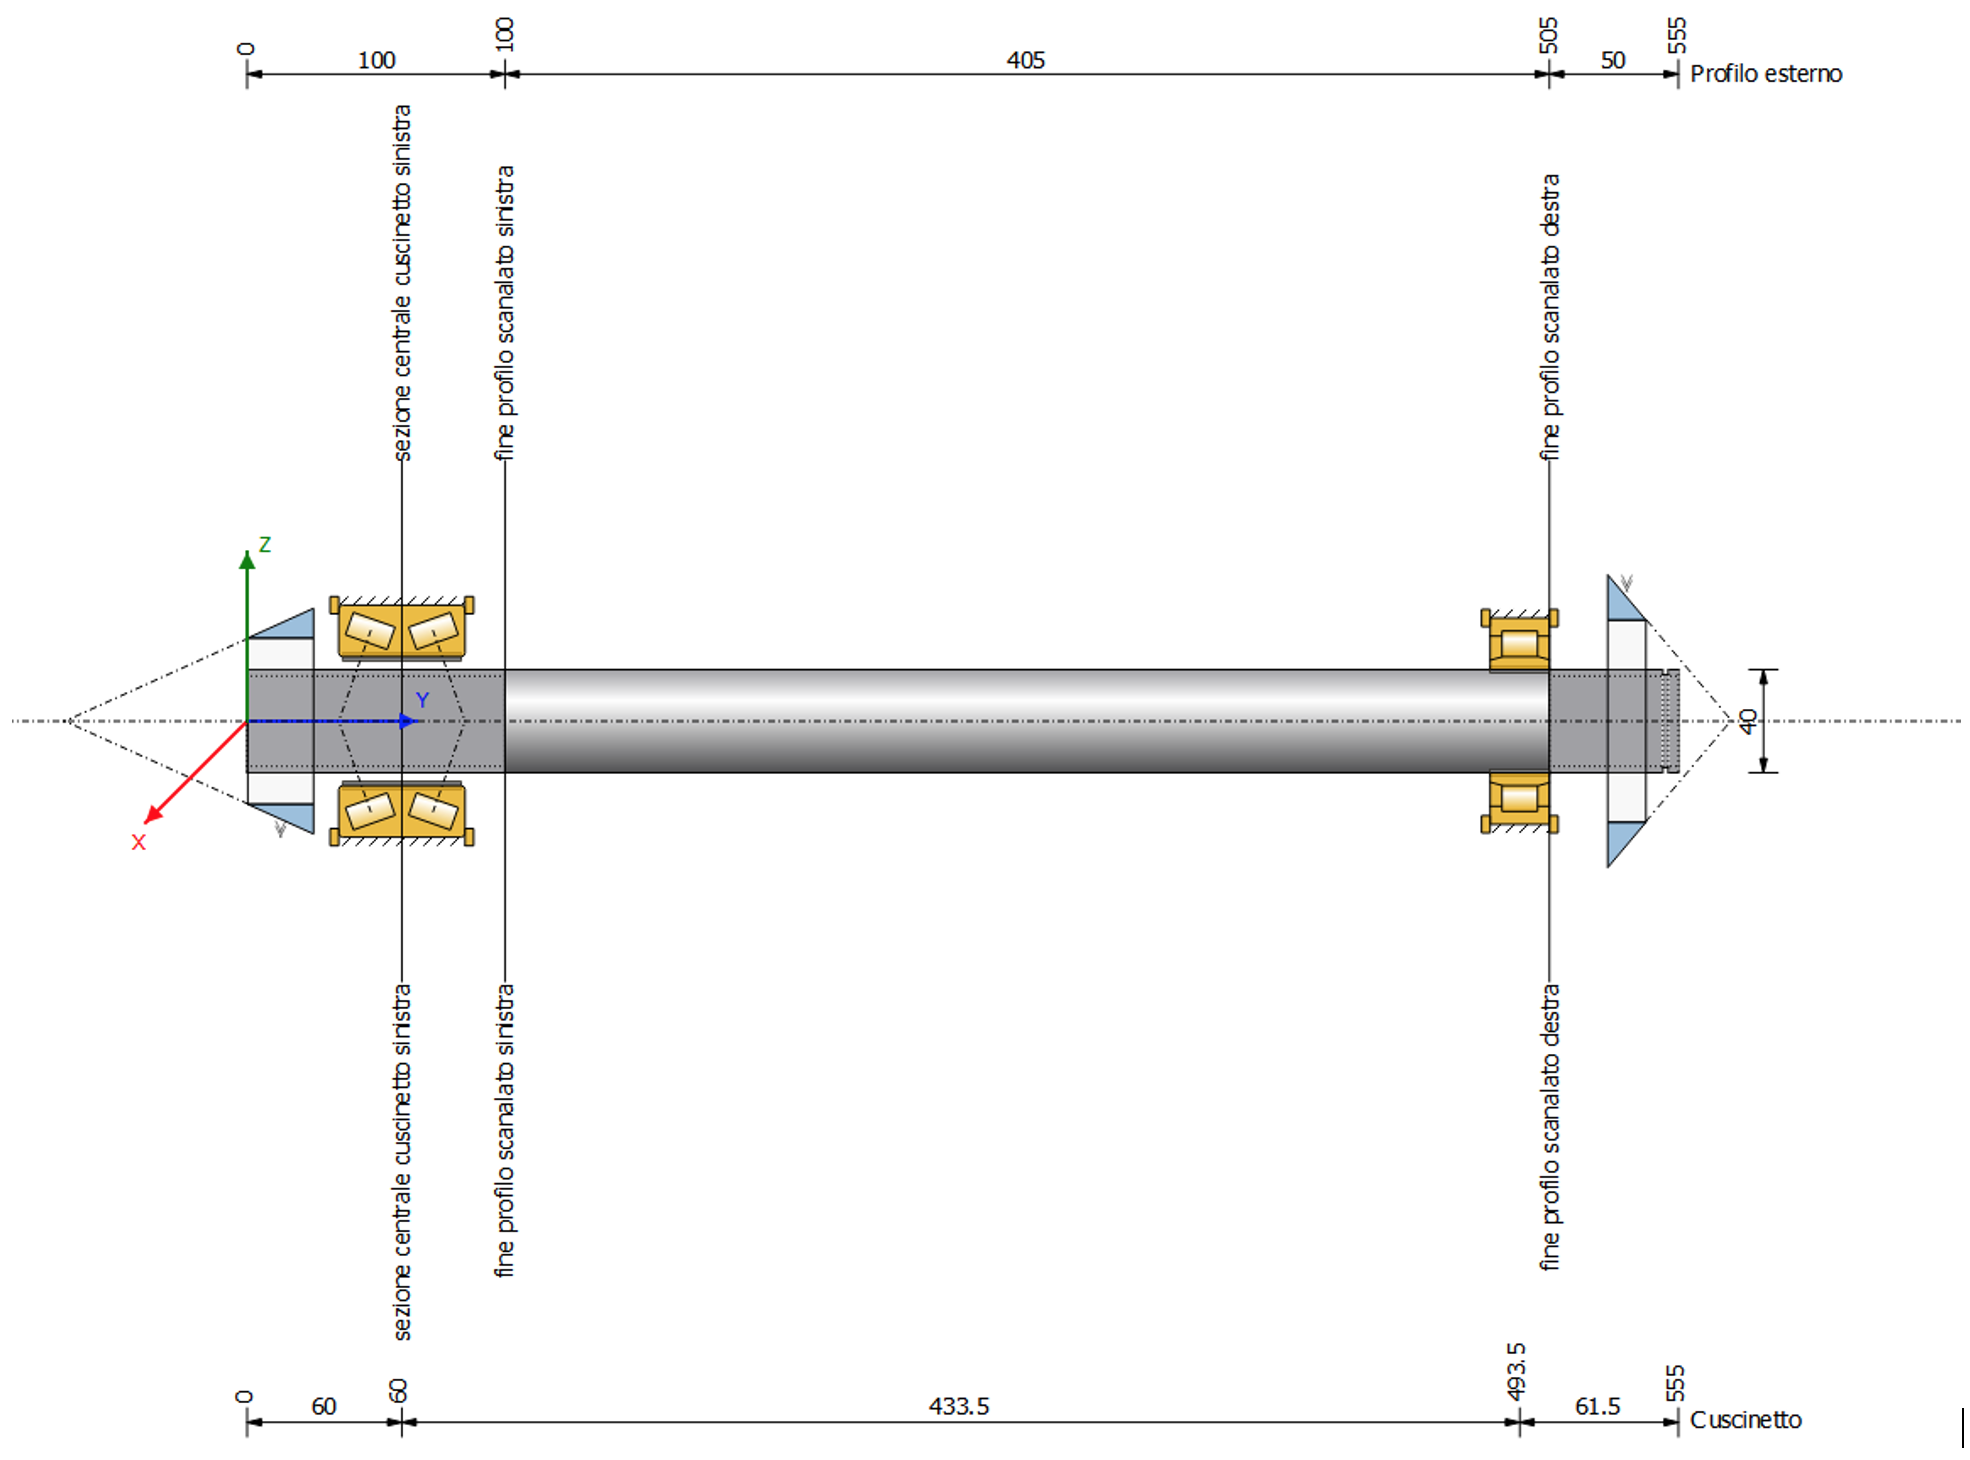
\includegraphics[scale=0.45]{Immagini/Albero2.png}
    \caption{Layout Albero 2}
    \label{fig:Albero2}
\end{figure}
\newpage

Il cuscinetto sinistro inserito possiede le seguenti caratteristiche
\begin{figure}[h]
    \centering
    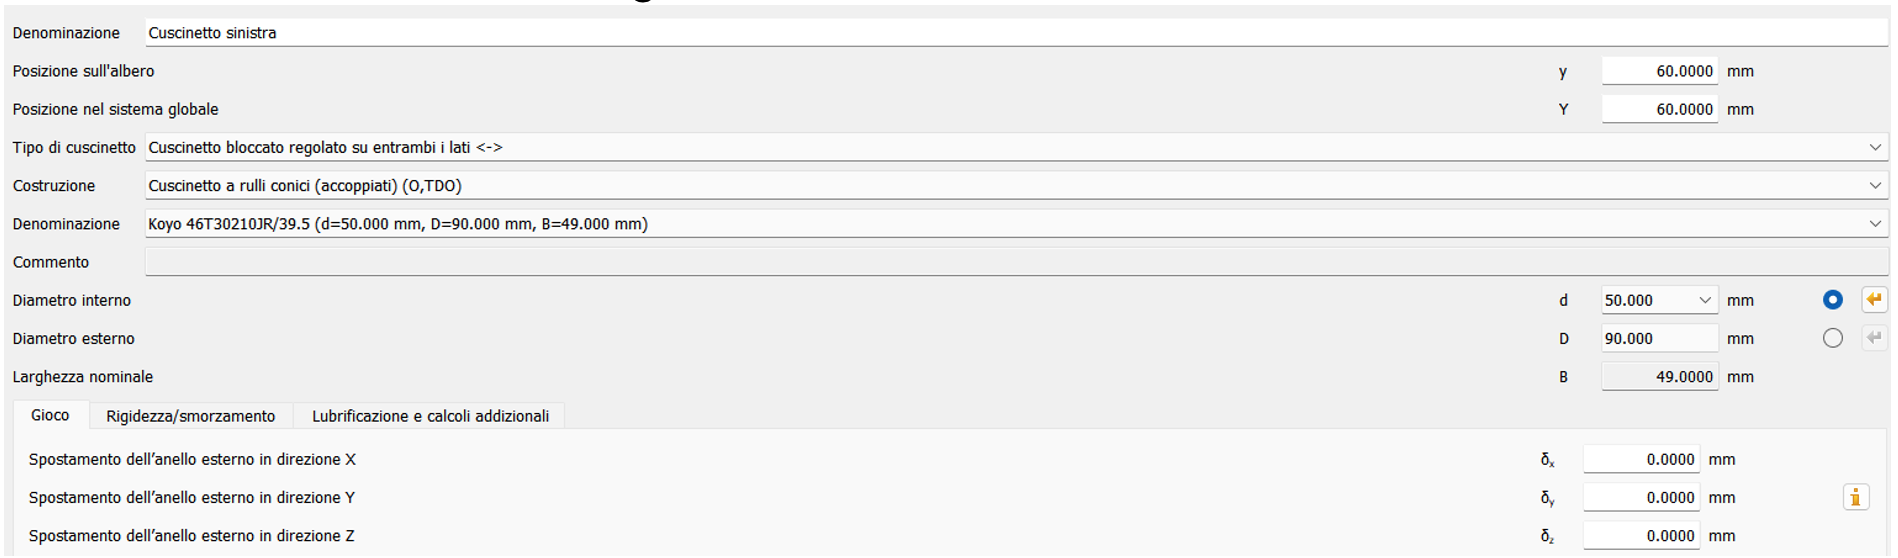
\includegraphics[scale=0.45]{Immagini/CuscinettoSinistraAlbero2.png}
    \caption{Caratteristiche cuscinetto sinistro relativo all'albero 2}
    \label{fig:CuscinettoSinsitraAlbero2}
\end{figure}

mentre il cuscinetto destro
\begin{figure}[h]
    \centering
    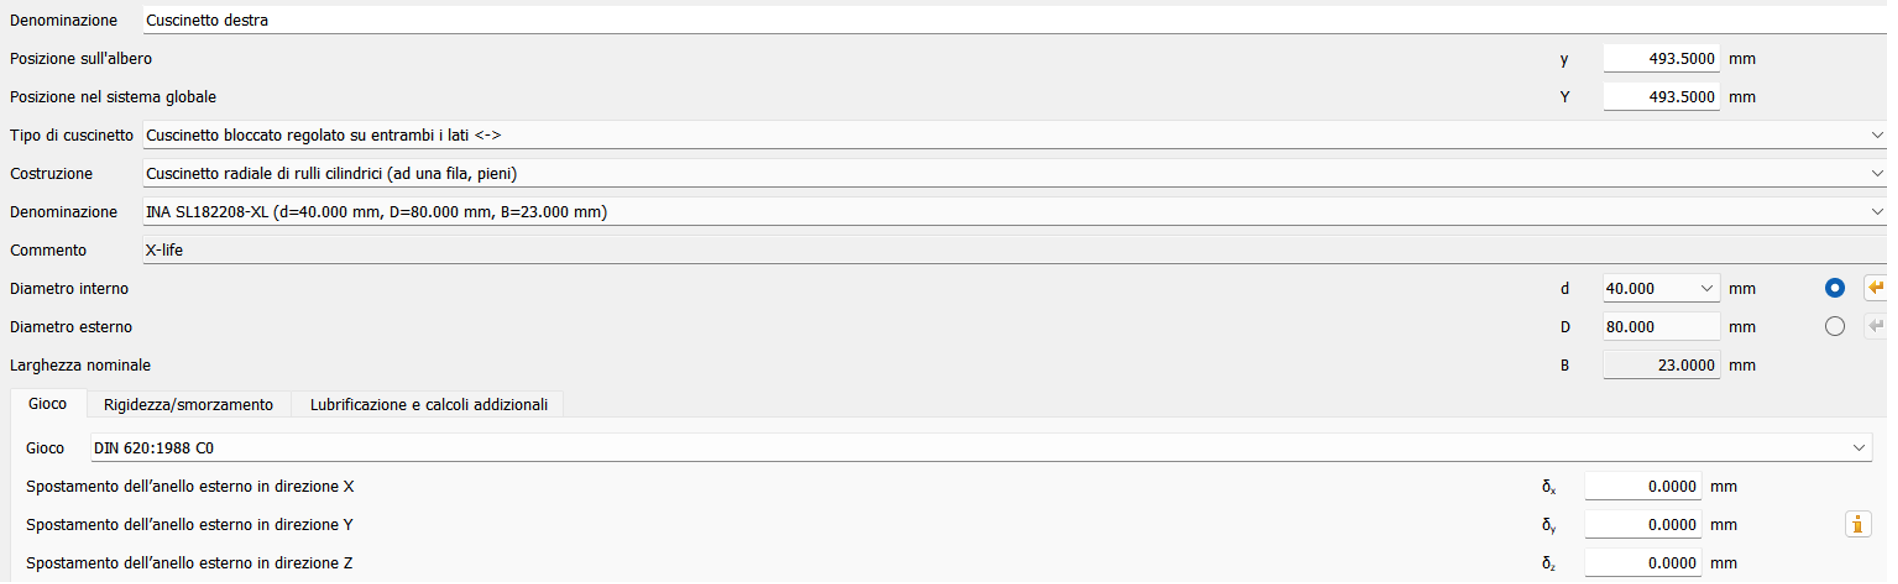
\includegraphics[scale=0.45]{Immagini/CuscinettoDestraAlbero2.png}
    \caption{Caratteristiche cuscinetto destro relativo all'albero 2}
    \label{fig:CuscinettoDestraAlbero2}
\end{figure}
\newpage
La prima ruota conica calettata sull'albero 2 corrisponde alla ruota 1, ed è la ruota da cui entra la coppia. Le caratteristiche di questa ruota sono riportate di seguito.
\begin{figure}[h]
    \centering
    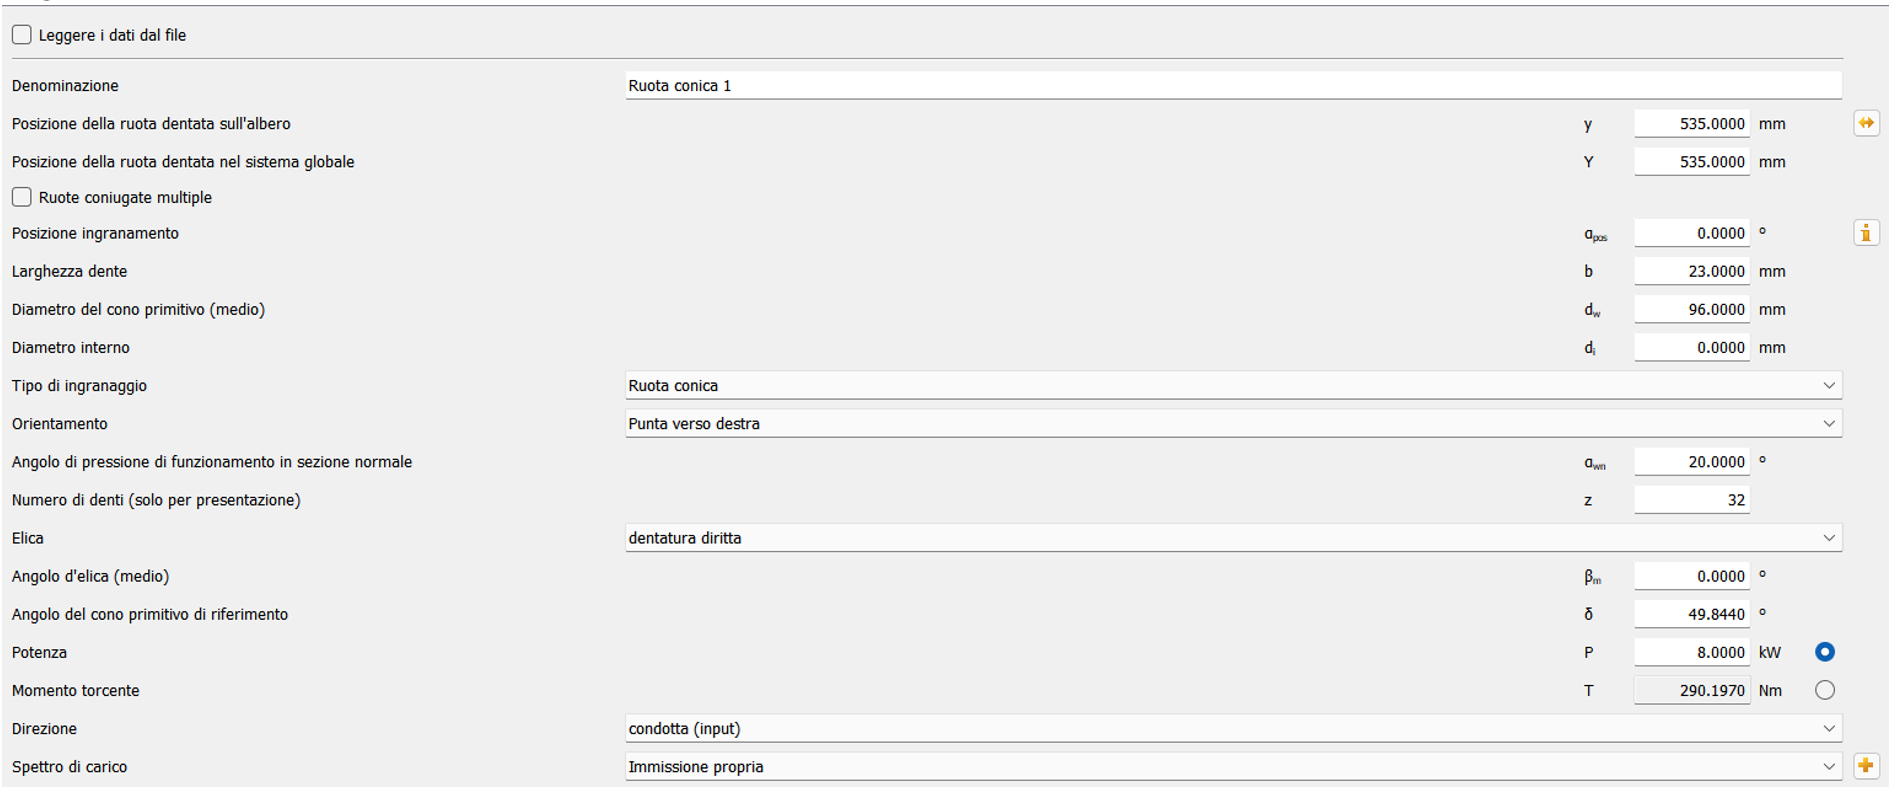
\includegraphics[scale=0.45]{Immagini/Ruota1Albero2.png}
    \caption{Dati della ruota 1 calettata sull'albero 2}
    \label{fig:Ruota1Albero2}
\end{figure}

L'elemento di output corrisponde alla ruota conica 3.
\begin{figure}[h]
    \centering
    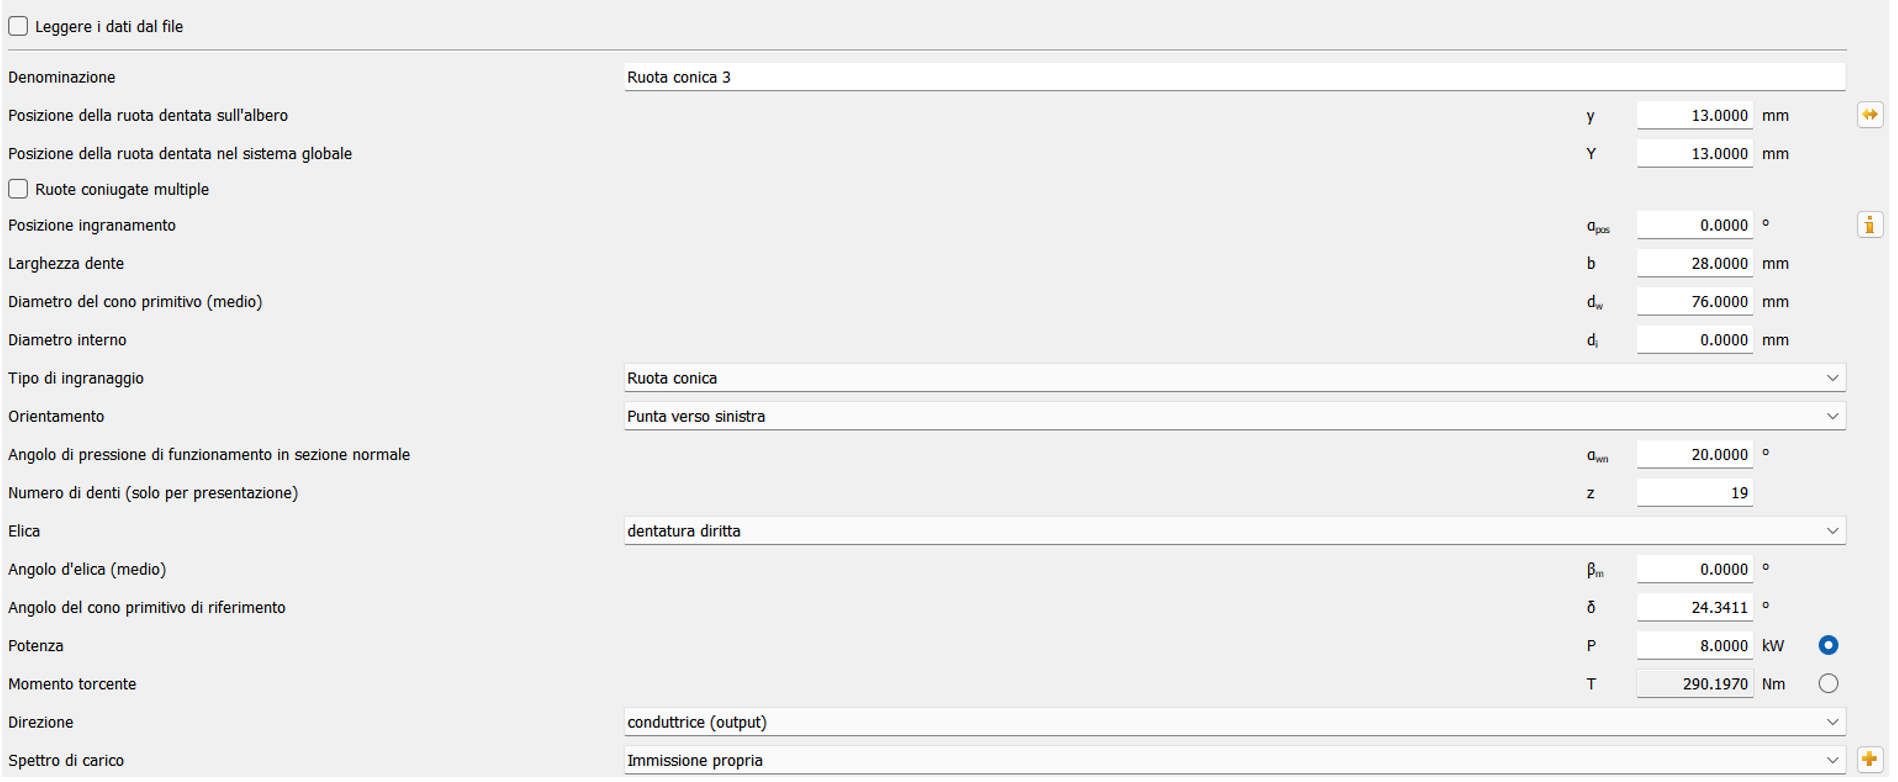
\includegraphics[scale=0.45]{Immagini/Ruota3Albero2.png}
    \caption{Dati della ruota 3 calettata sull'albero2}
    \label{fig:Ruota3Albero2}
    \end{figure}
\newpage
Sono state poi considerate le grandezze di dettaglio:
\begin{figure}[h]
    \centering
    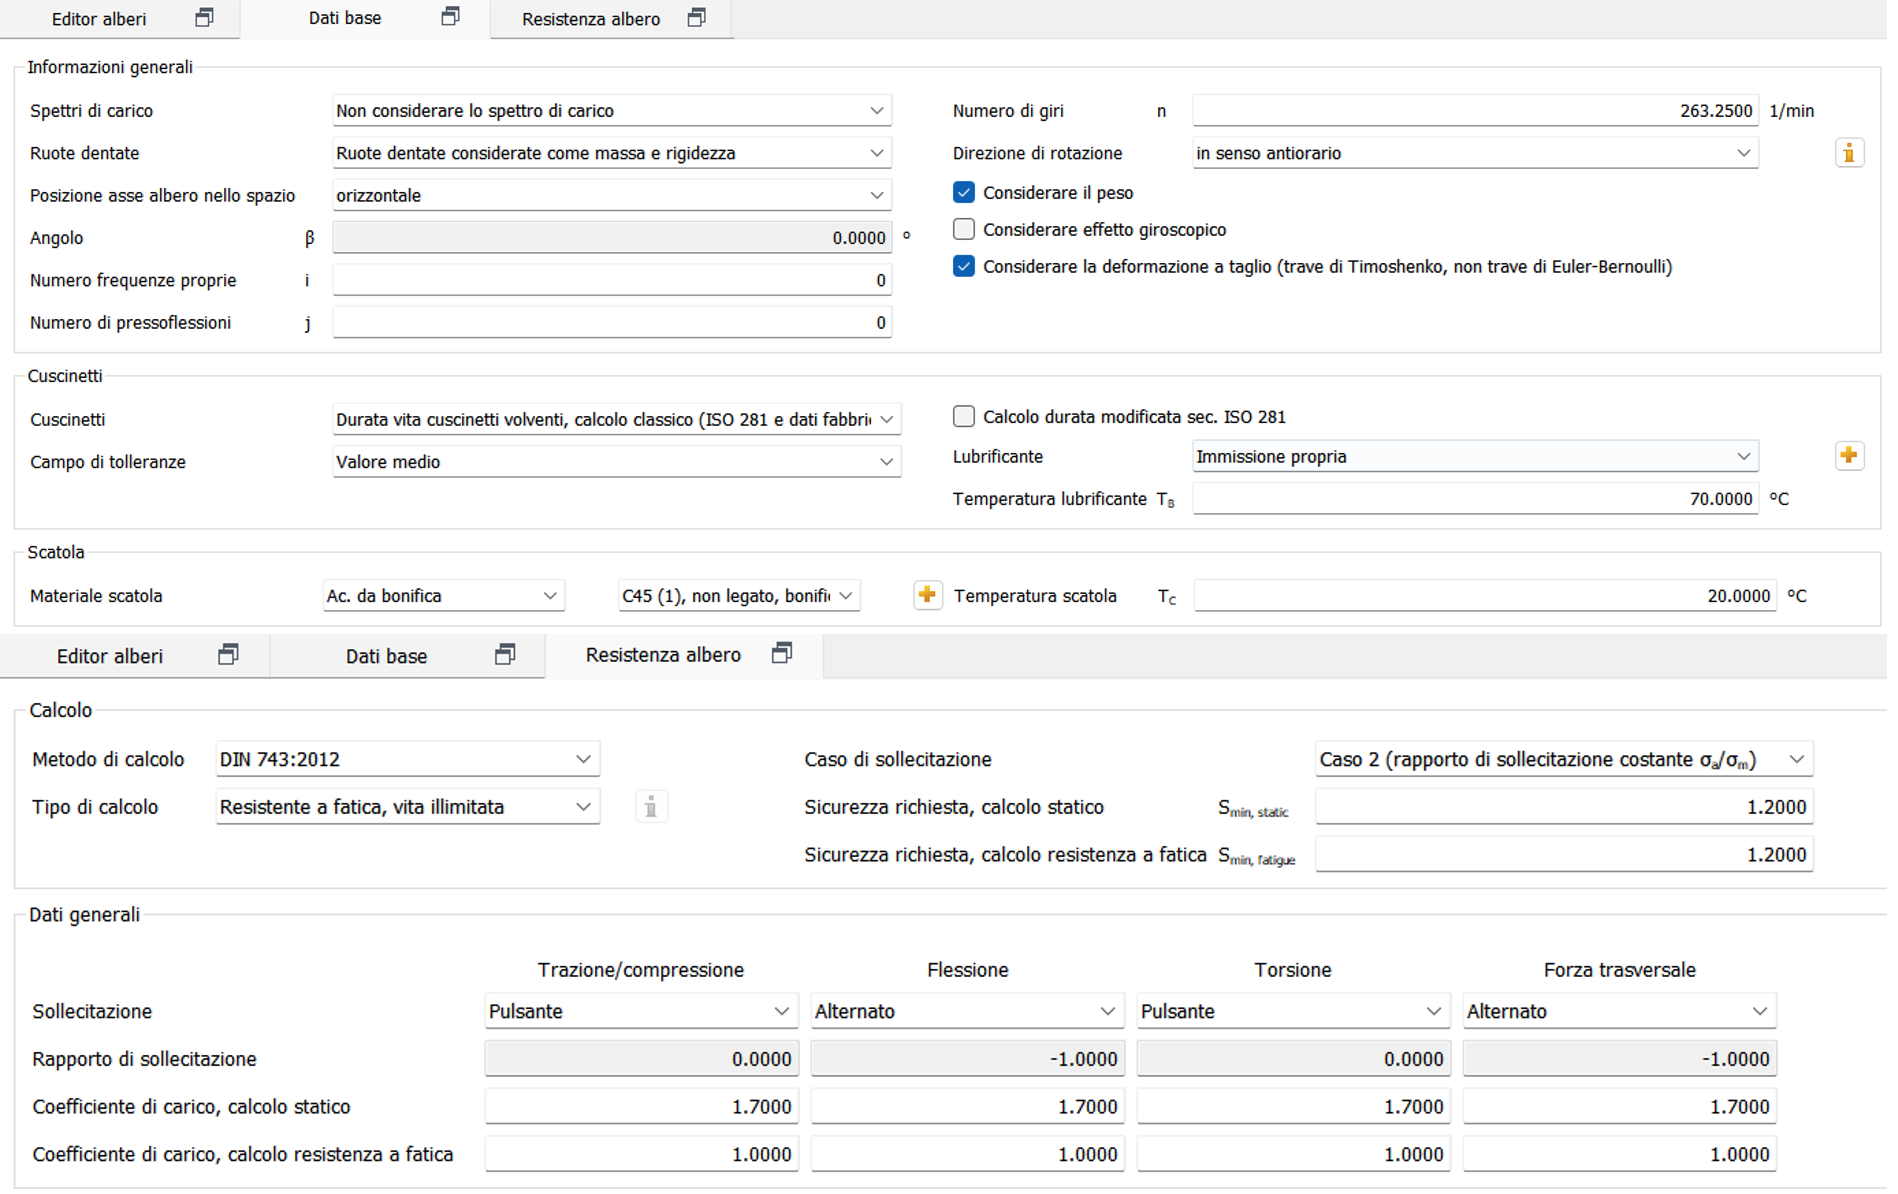
\includegraphics[scale=0.45]{Immagini/DettagliAlbero2.png}
    \caption{Grandezze di dettaglio relative all'analisi dell'albero 2}
    \label{fig:DettagliAlbero2}
\end{figure}

Dal Report fornito dal software è possibile ottenere ulteriori informazioni di interesse sull'albero appena progettato. 

\emph{Applicazione del carico}
\begin{figure}[h]
    \centering
    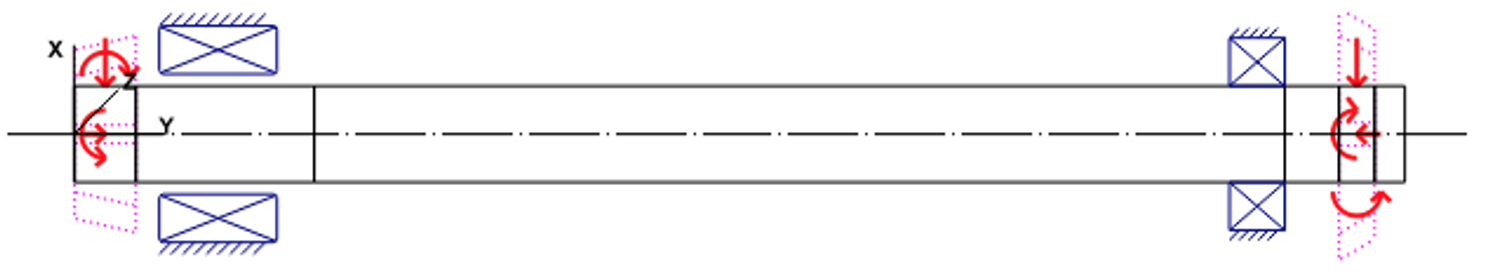
\includegraphics[scale=0.5]{Immagini/CaricoAlbero2.png}
    \caption{Applicazione del carico lungo l'albero 2}
    \label{fig:CaricoAlbero2}
\end{figure}
\newpage
\emph{Forze agenti sulle ruote}
\begin{figure}[h]
    \centering
    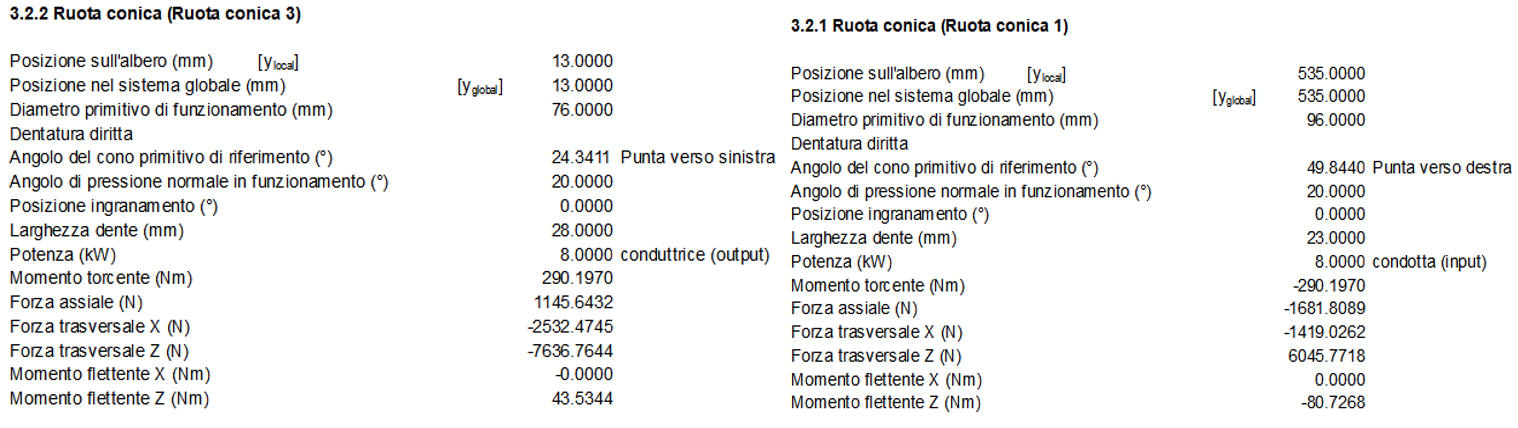
\includegraphics[scale=0.5]{Immagini/ForzeRuoteAlbero2.png}
    \caption{Valore delle forze trasmesse sull'albero 2}
    \label{fig:ForzeRuoteAlbero2}
\end{figure}

\emph{Dettagli cuscinetti}
\begin{figure}[h]
    \centering
    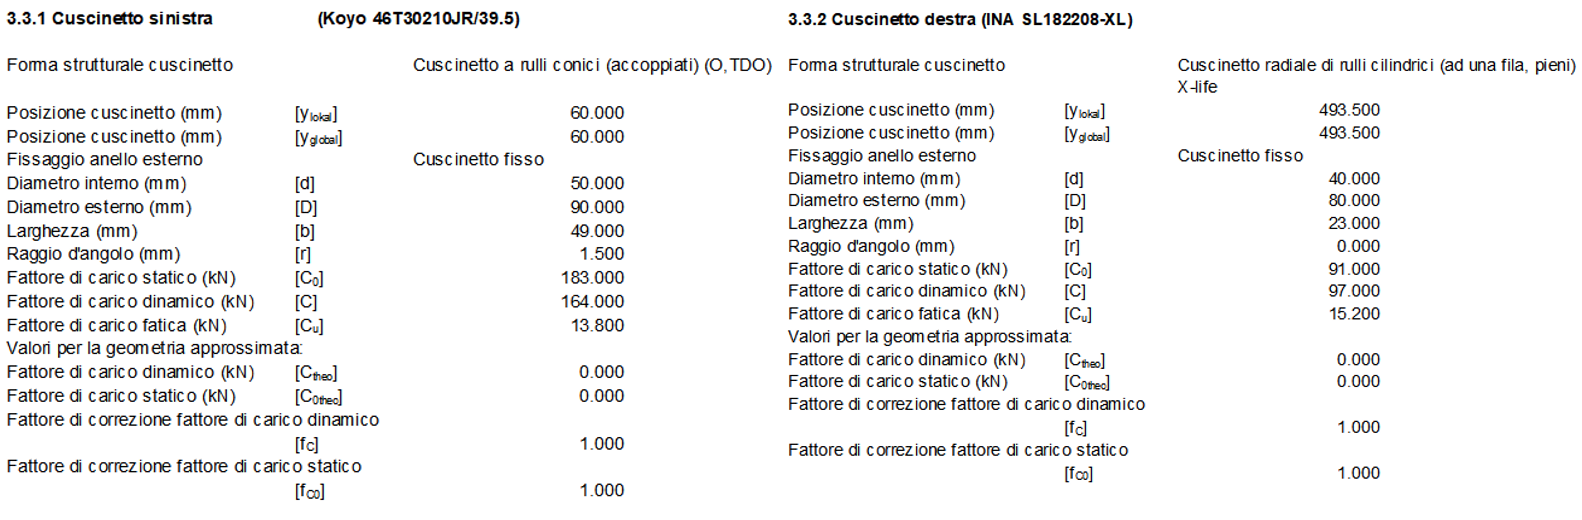
\includegraphics[scale=0.5]{Immagini/ForzeCuscinettiAlbero2.png}
    \caption{Valore delle forze trasmesse sull'albero 2}
    \label{fig:ForzeCusinettiAlbero2}
\end{figure}

\emph{Deformazione dell'albero}
\begin{figure}[h]
    \centering
    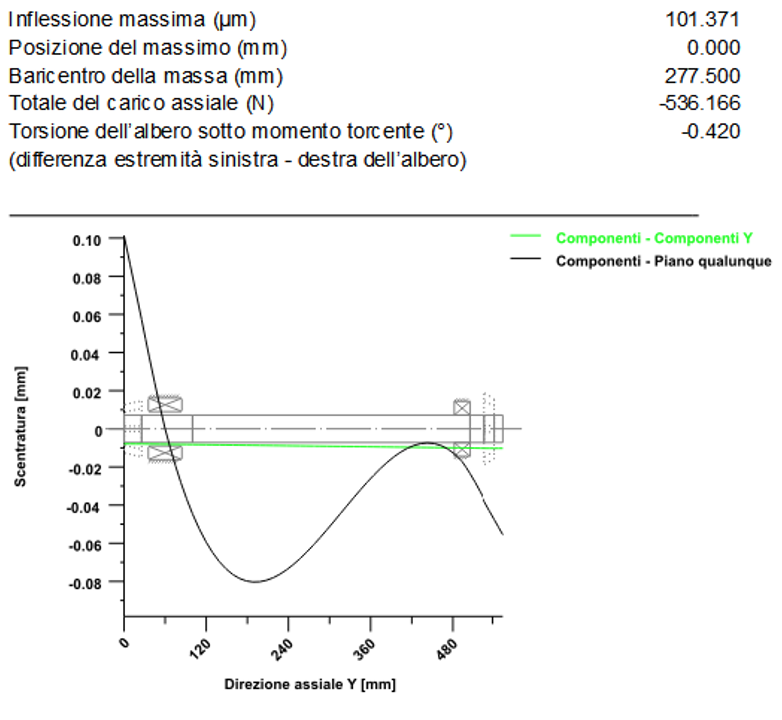
\includegraphics[scale=0.45]{Immagini/DeformataAlbero2.png}
    \caption{Deformata dell'albero 2}
    \label{fig:Deformata albero 2}
\end{figure}
\newpage
\emph{Andamento della tensione equivalente}
\begin{figure}[h]
    \centering
    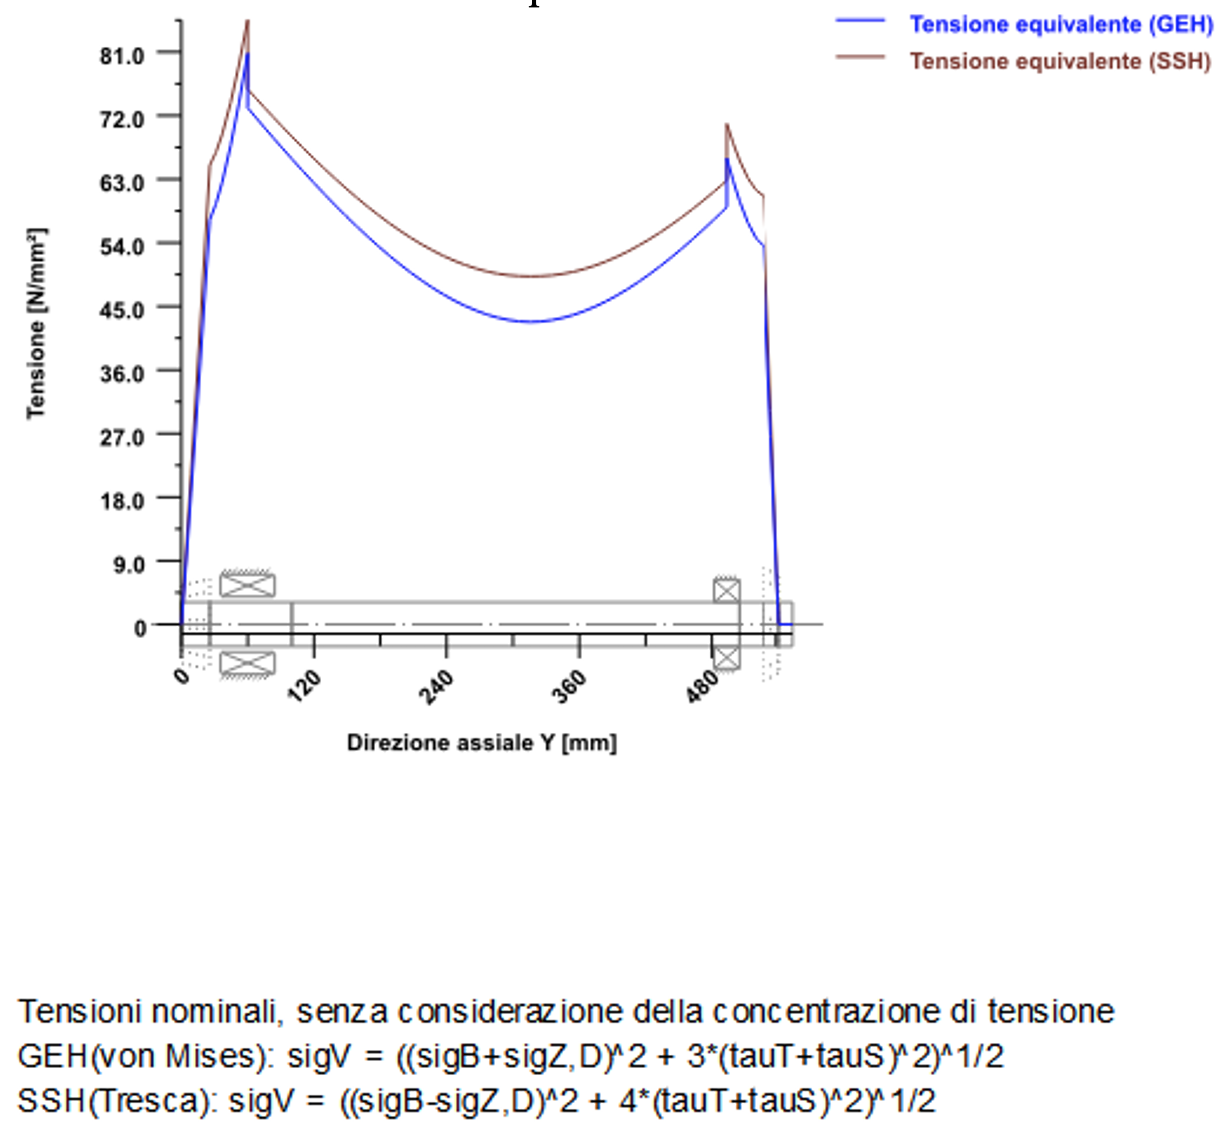
\includegraphics[scale=0.5]{Immagini/TensioniAlbero2.png}
    \caption{Andamento della tensione equivalente lungo l'albero 2}
    \label{fig:TensioniAlbero2}
\end{figure}

Infine, attraverso la compilazione del software si è osservato come tutte le sezioni fossero ampiamente verificate sia staticamente che a fatica.
\begin{figure}[h]
    \centering
    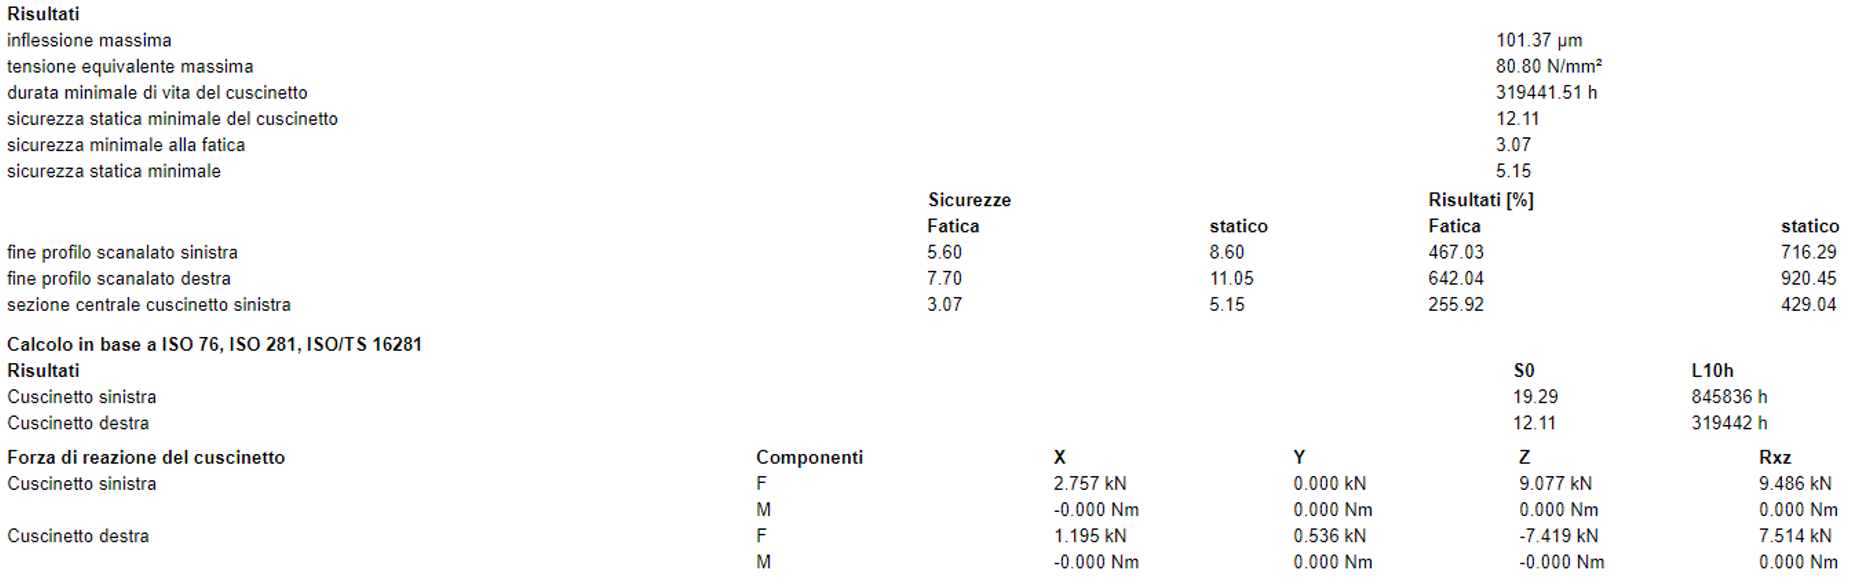
\includegraphics[scale=0.4]{Immagini/RisultatiAlbero2.png}
    \caption{Risultato dell'analisi statica e a fatica delle sezioni di interesse dell'albero 2}
    \label{fig:RisultatiALbero2}
\end{figure}

\paragraph{Albero 3}
\begin{figure}[h]
    \centering
    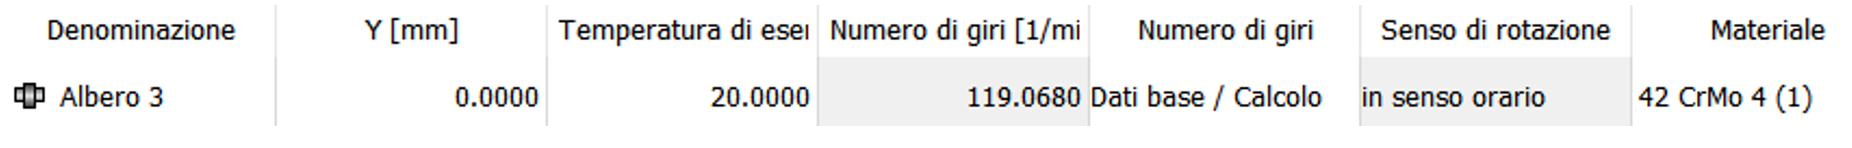
\includegraphics[scale=0.4]{Immagini/DatiAlbero3.png}
    \caption{Albero  3}
    \label{fig:DatiAlbero3}
\end{figure}

Sono state individuate quattro sezioni di interesse:
\begin{itemize}
    \item Due sezioni per le gole di scarico (cuscinetto di destra e sinistra);
    \item Due sezioni in corrispondenza dei raggi di raccordo degli spallamenti;
\end{itemize}
\newpage
\begin{figure}[h]
    \centering
    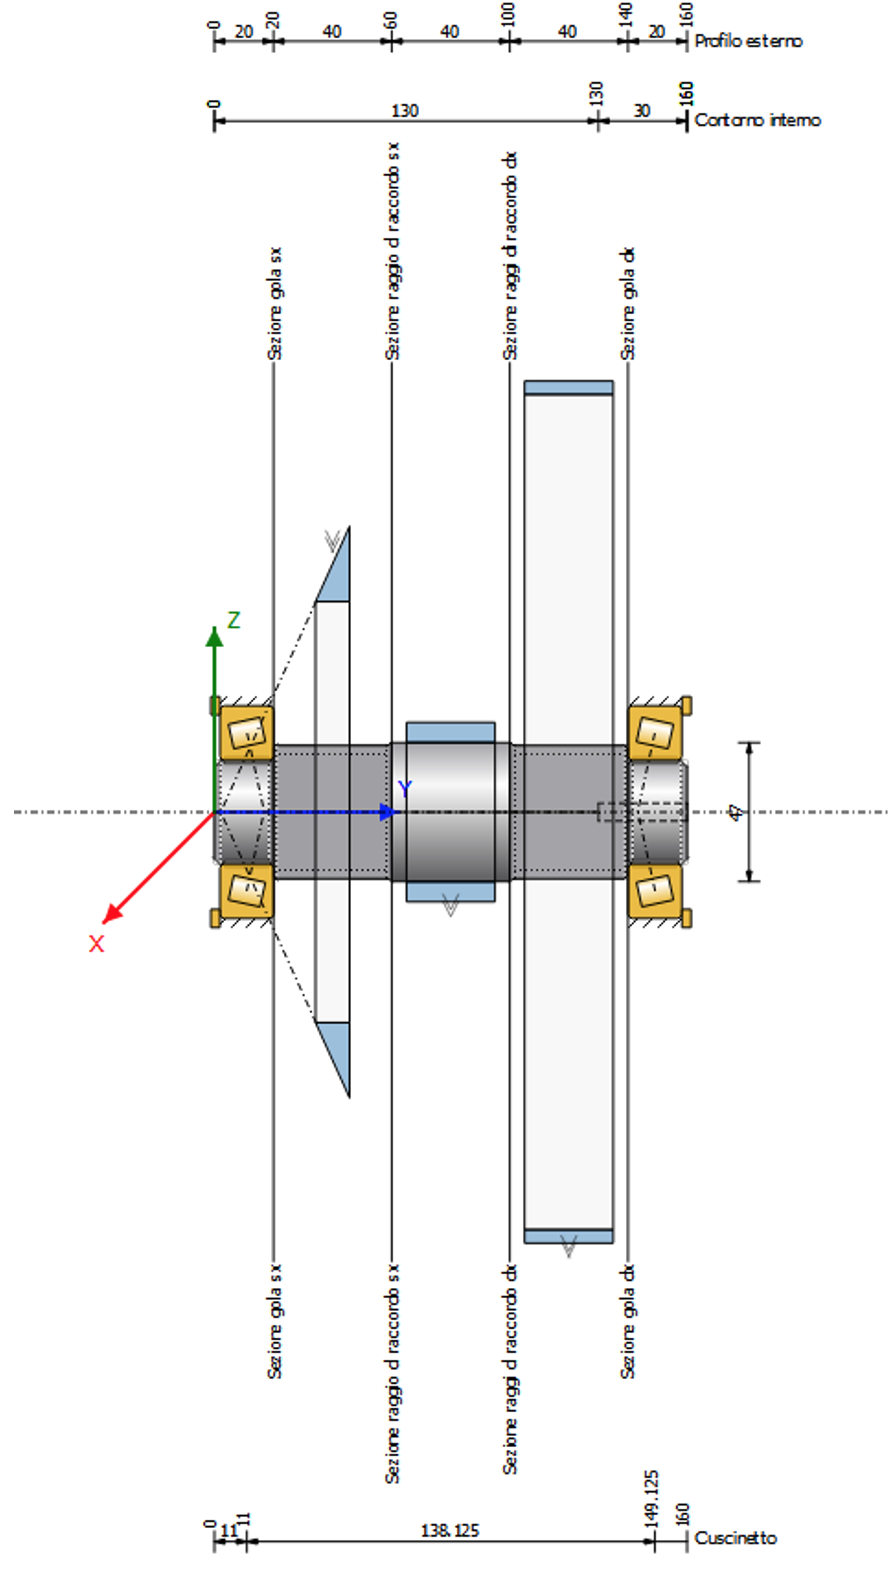
\includegraphics[scale=0.52]{Immagini/Albero3.png}
    \caption{Layout Albero 3}
    \label{fig:Albero3}
\end{figure}
\newpage

Il cuscinetto sinistro inserito possiede le seguenti caratteristiche
\begin{figure}[h]
    \centering
    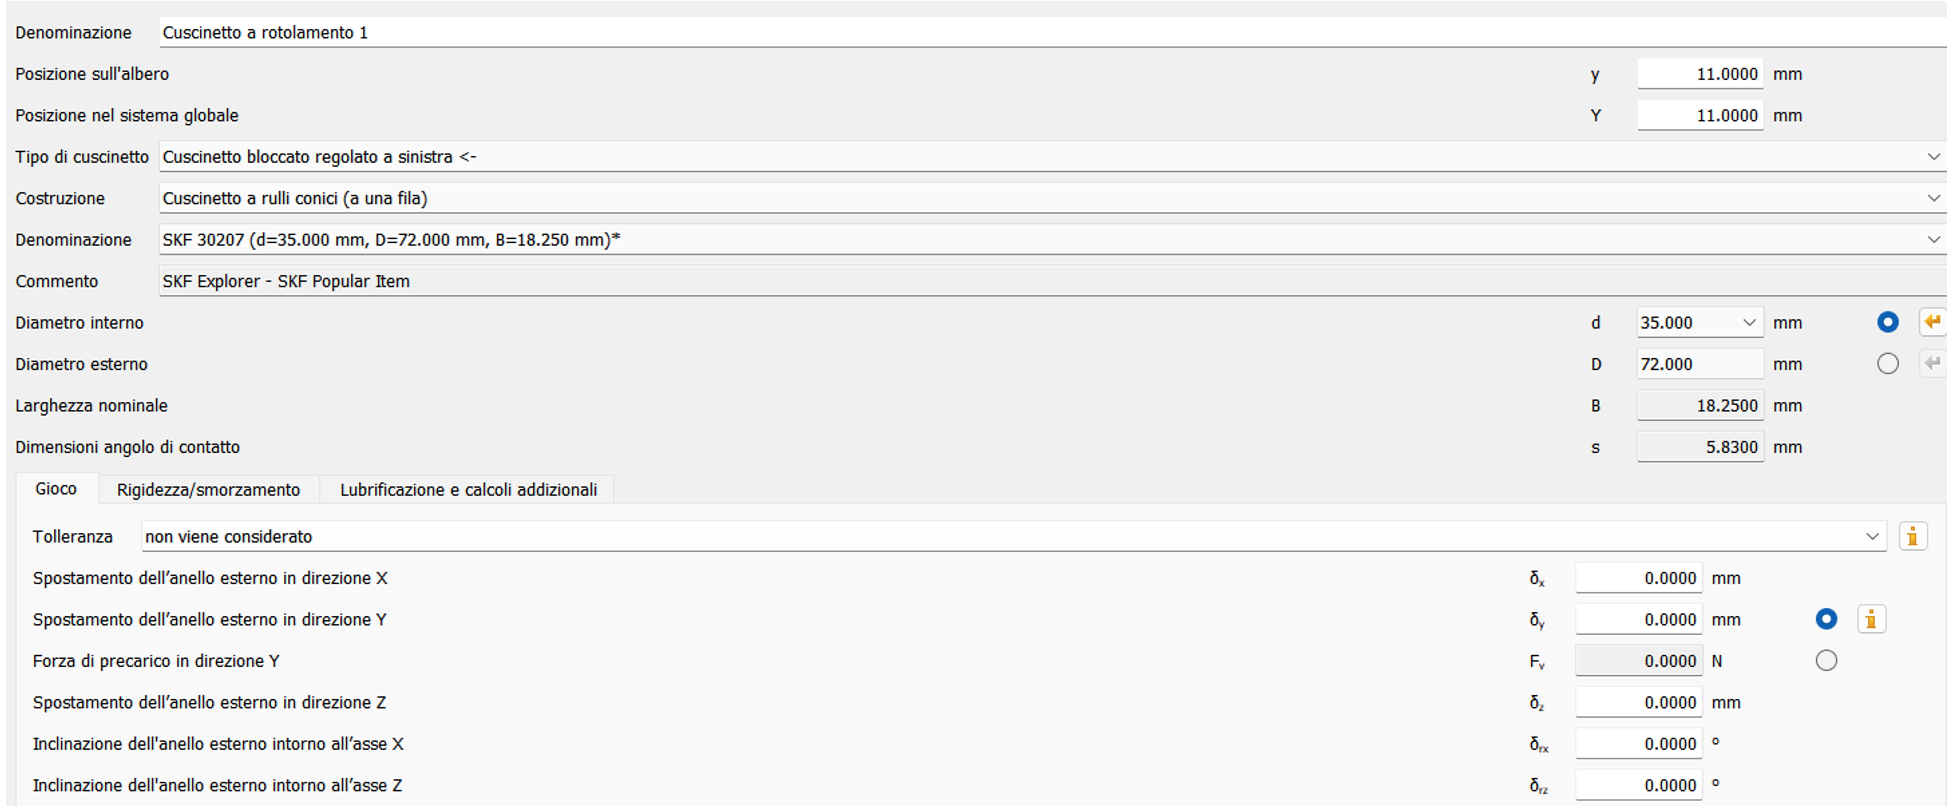
\includegraphics[scale=0.45]{Immagini/CuscinettoSinistraAlbero3.png}
    \caption{Caratteristiche cuscinetto sinistro relativo all'albero 3}
    \label{fig:CuscinettoSinsitraAlbero3}
\end{figure}

mentre il cuscinetto destro
\begin{figure}[h]
    \centering
    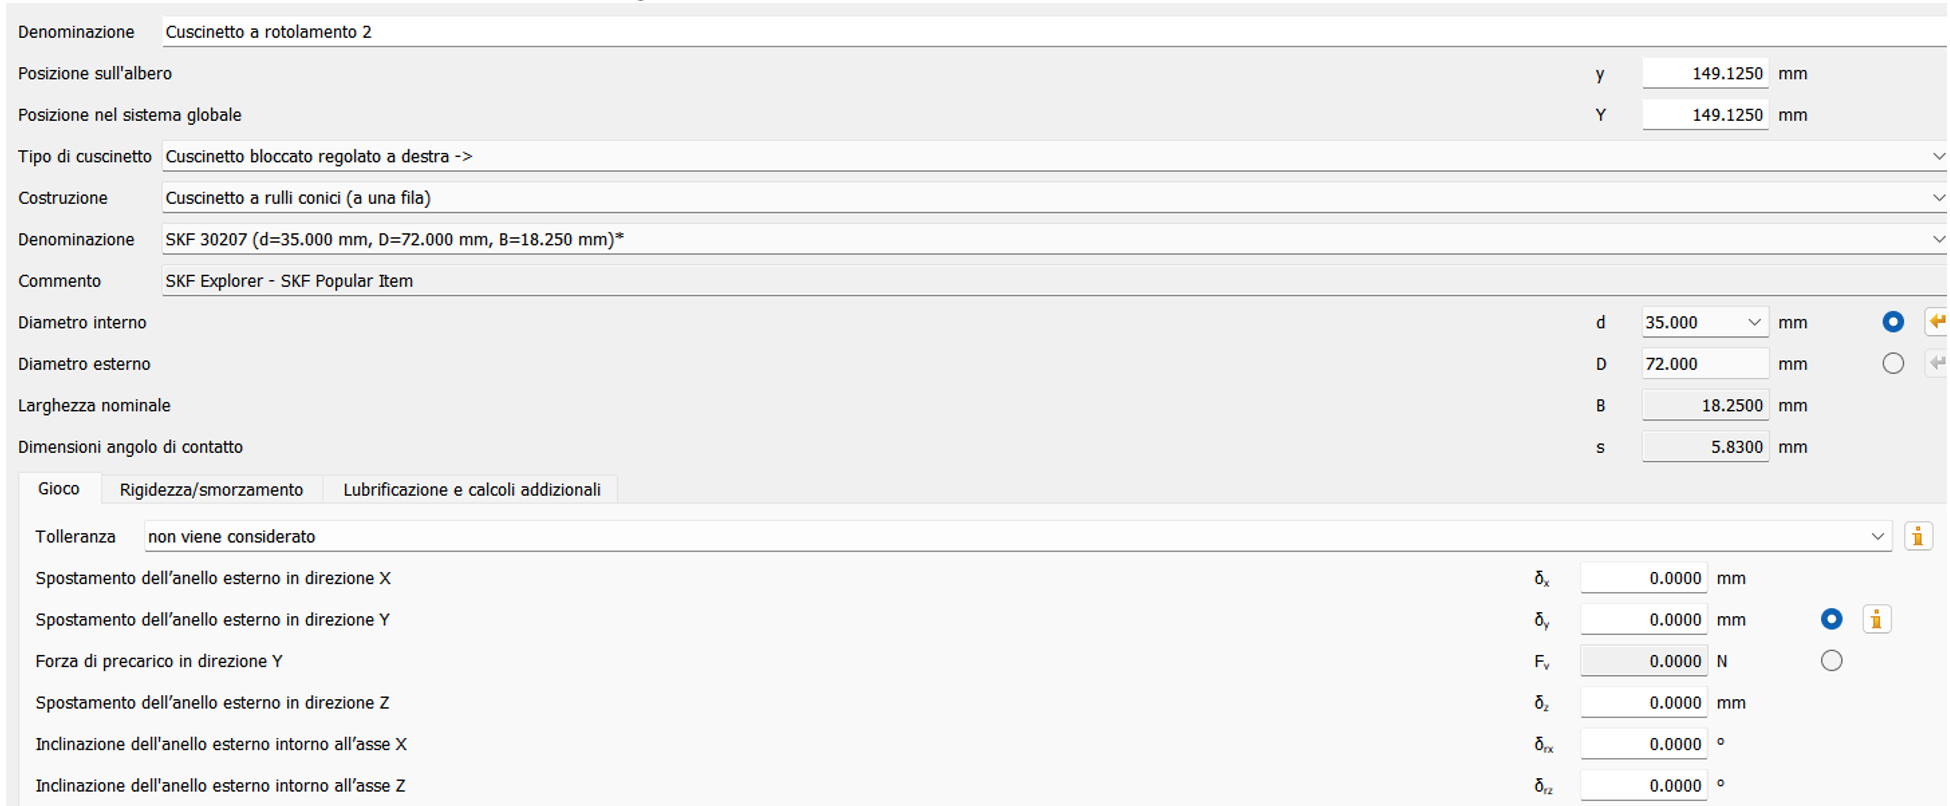
\includegraphics[scale=0.45]{Immagini/CuscinettoDestraAlbero3.png}
    \caption{Caratteristiche cuscinetto destro relativo all'albero 3}
    \label{fig:CuscinettoDestraAlbero3}
\end{figure}
\newpage
La prima ruota conica calettata sull'albero 3 corrisponde alla ruota 3, ed è la ruota da cui entra la coppia. Le caratteristiche di questa ruota sono riportate di seguito.
\begin{figure}[h]
    \centering
    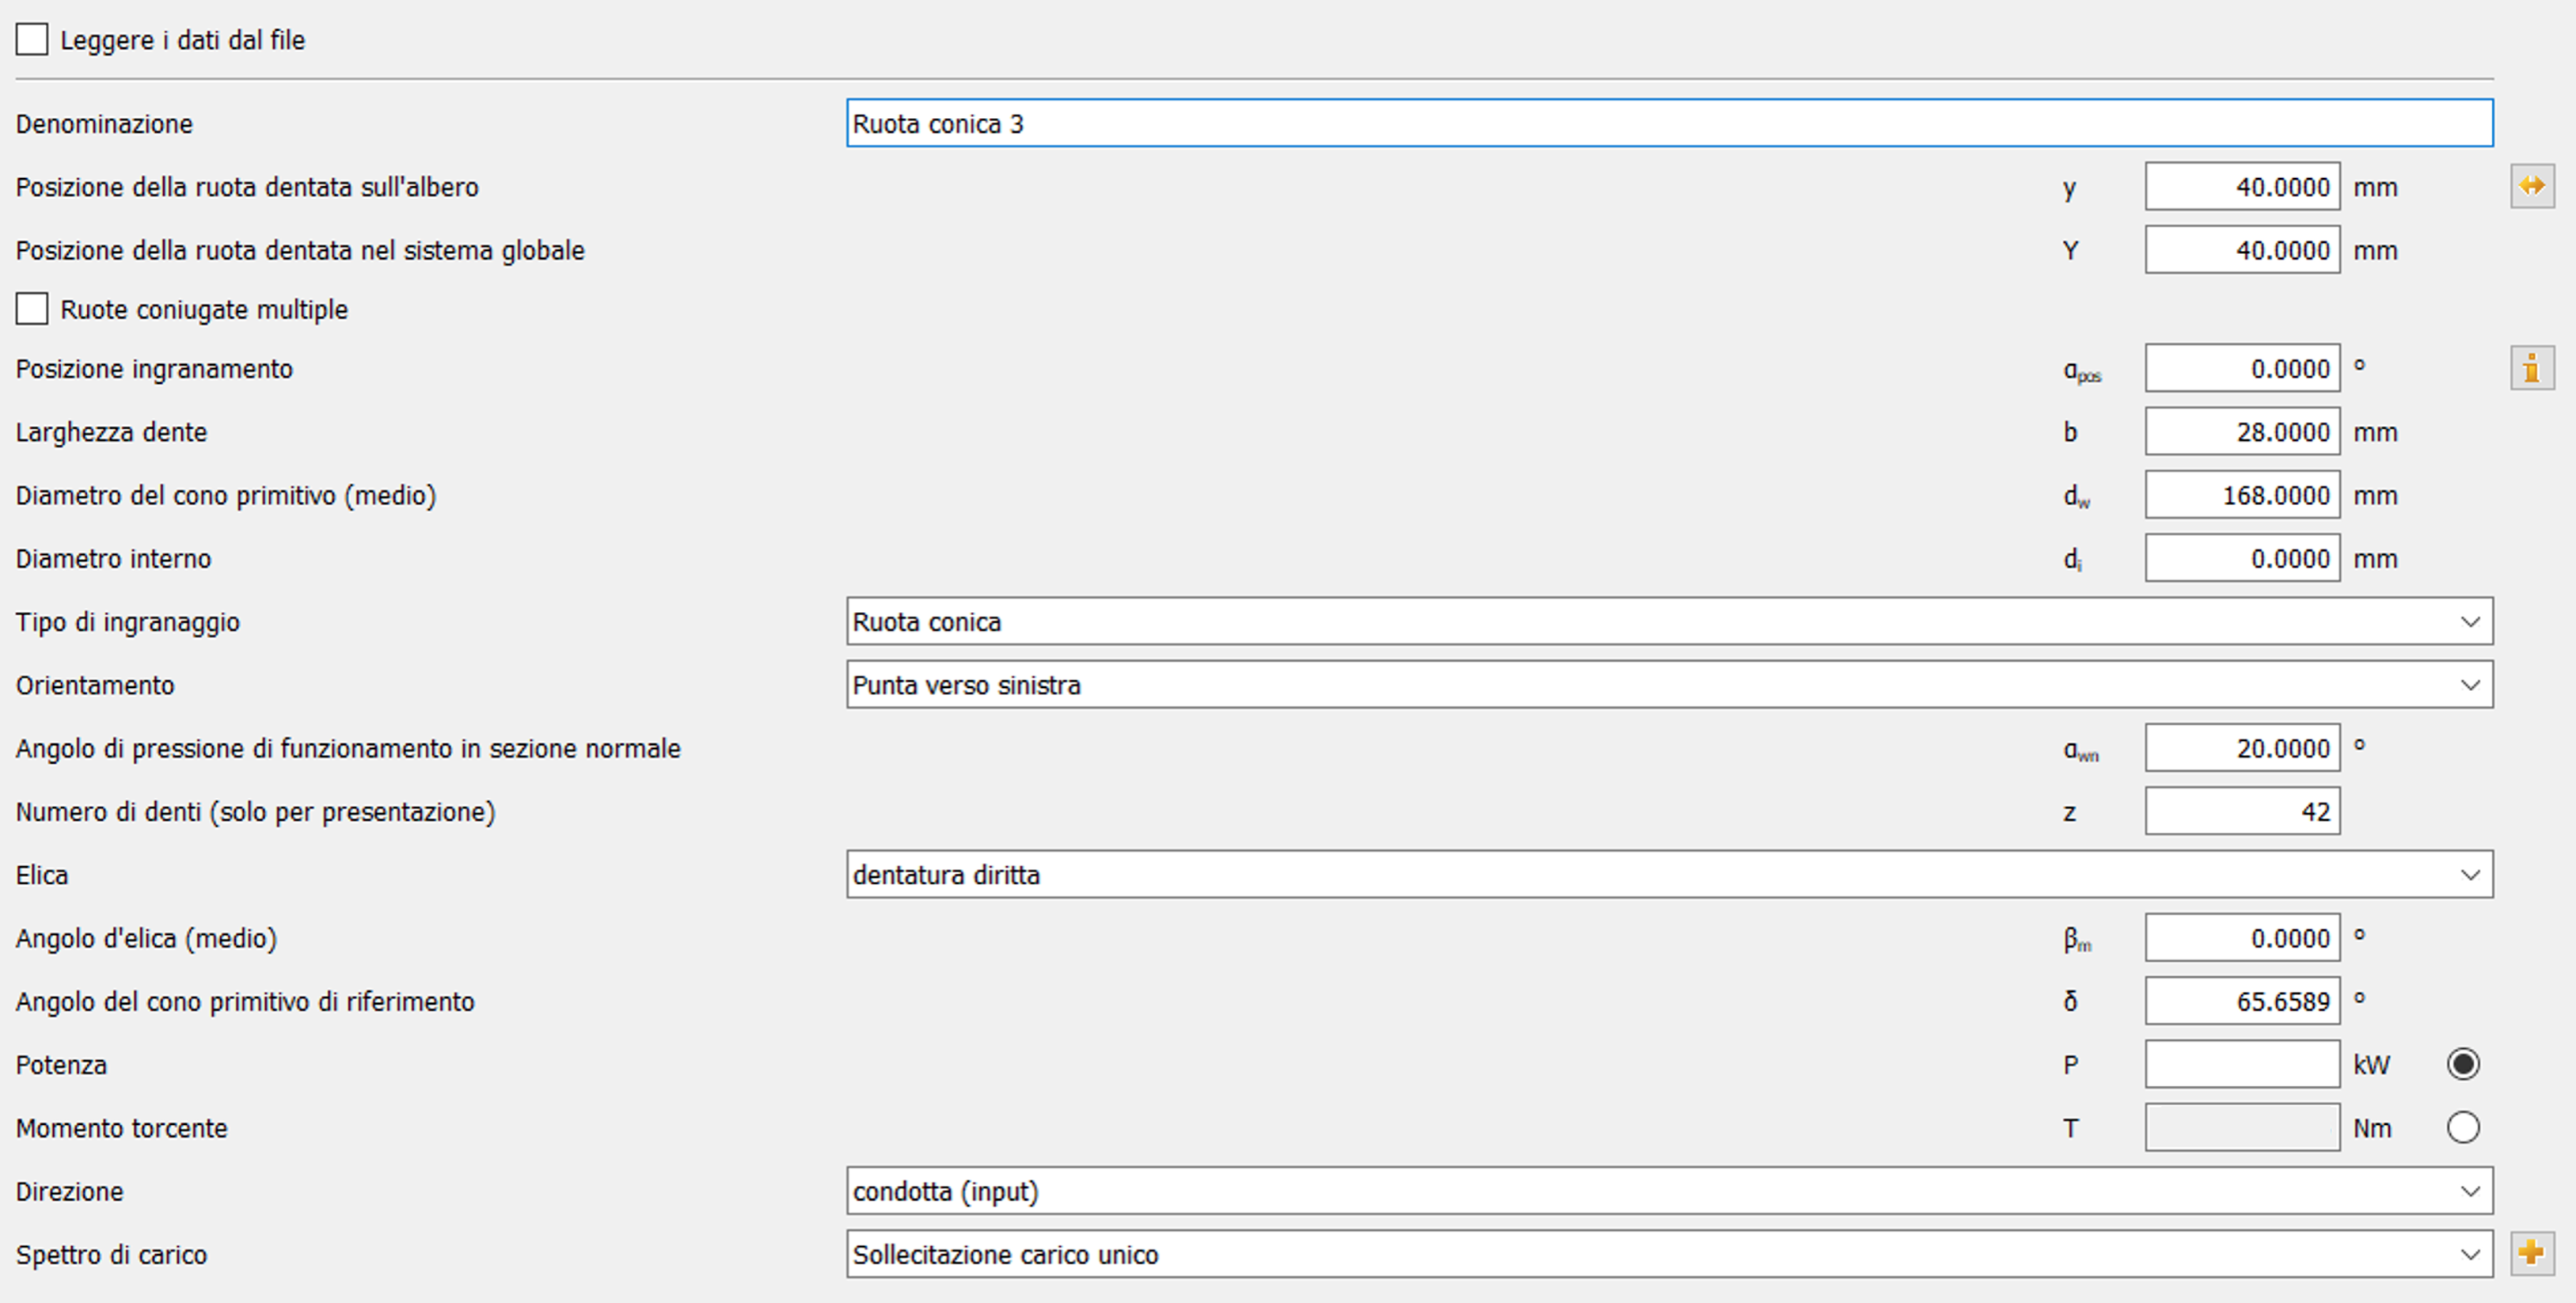
\includegraphics[scale=0.27]{Immagini/Ruota3Albero3.png}
    \caption{Dati della ruota 3 calettata sull'albero 3}
    \label{fig:Ruota1Albero2}
\end{figure}
\newpage
Le due ruote denominate 4 e 6 distribuiscono la coppia in ingresso ai due output del riduttore. La due ruote presentano le seguenti caratteristiche.
\begin{figure}[h]
    \centering
    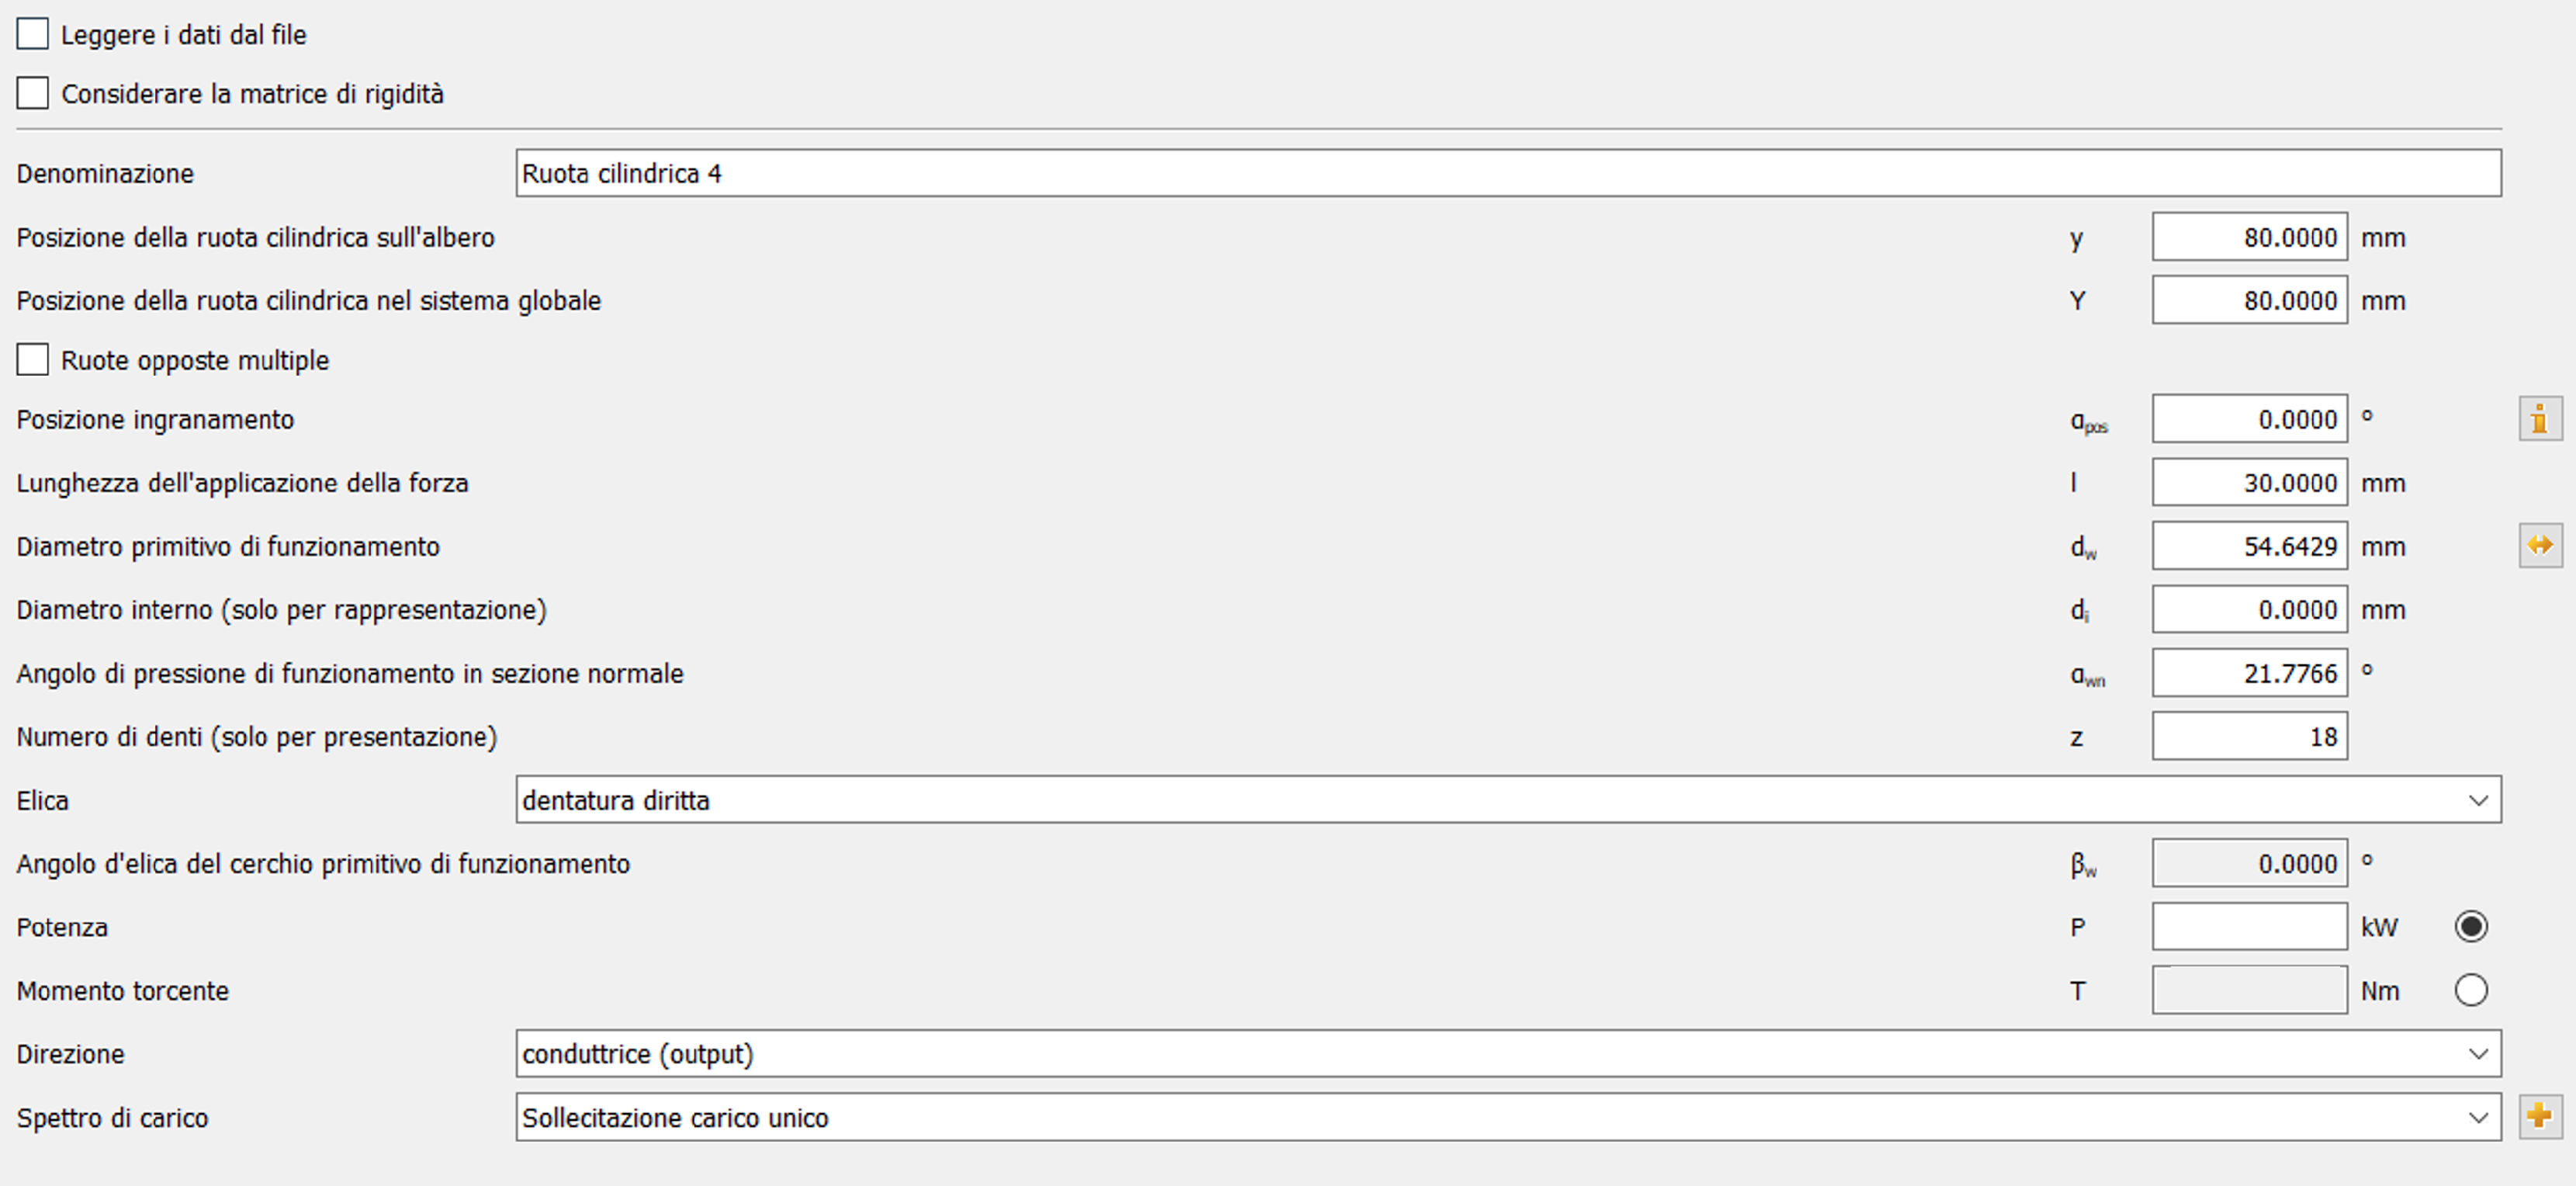
\includegraphics[scale=0.27]{Immagini/Ruota4Albero3.png}
    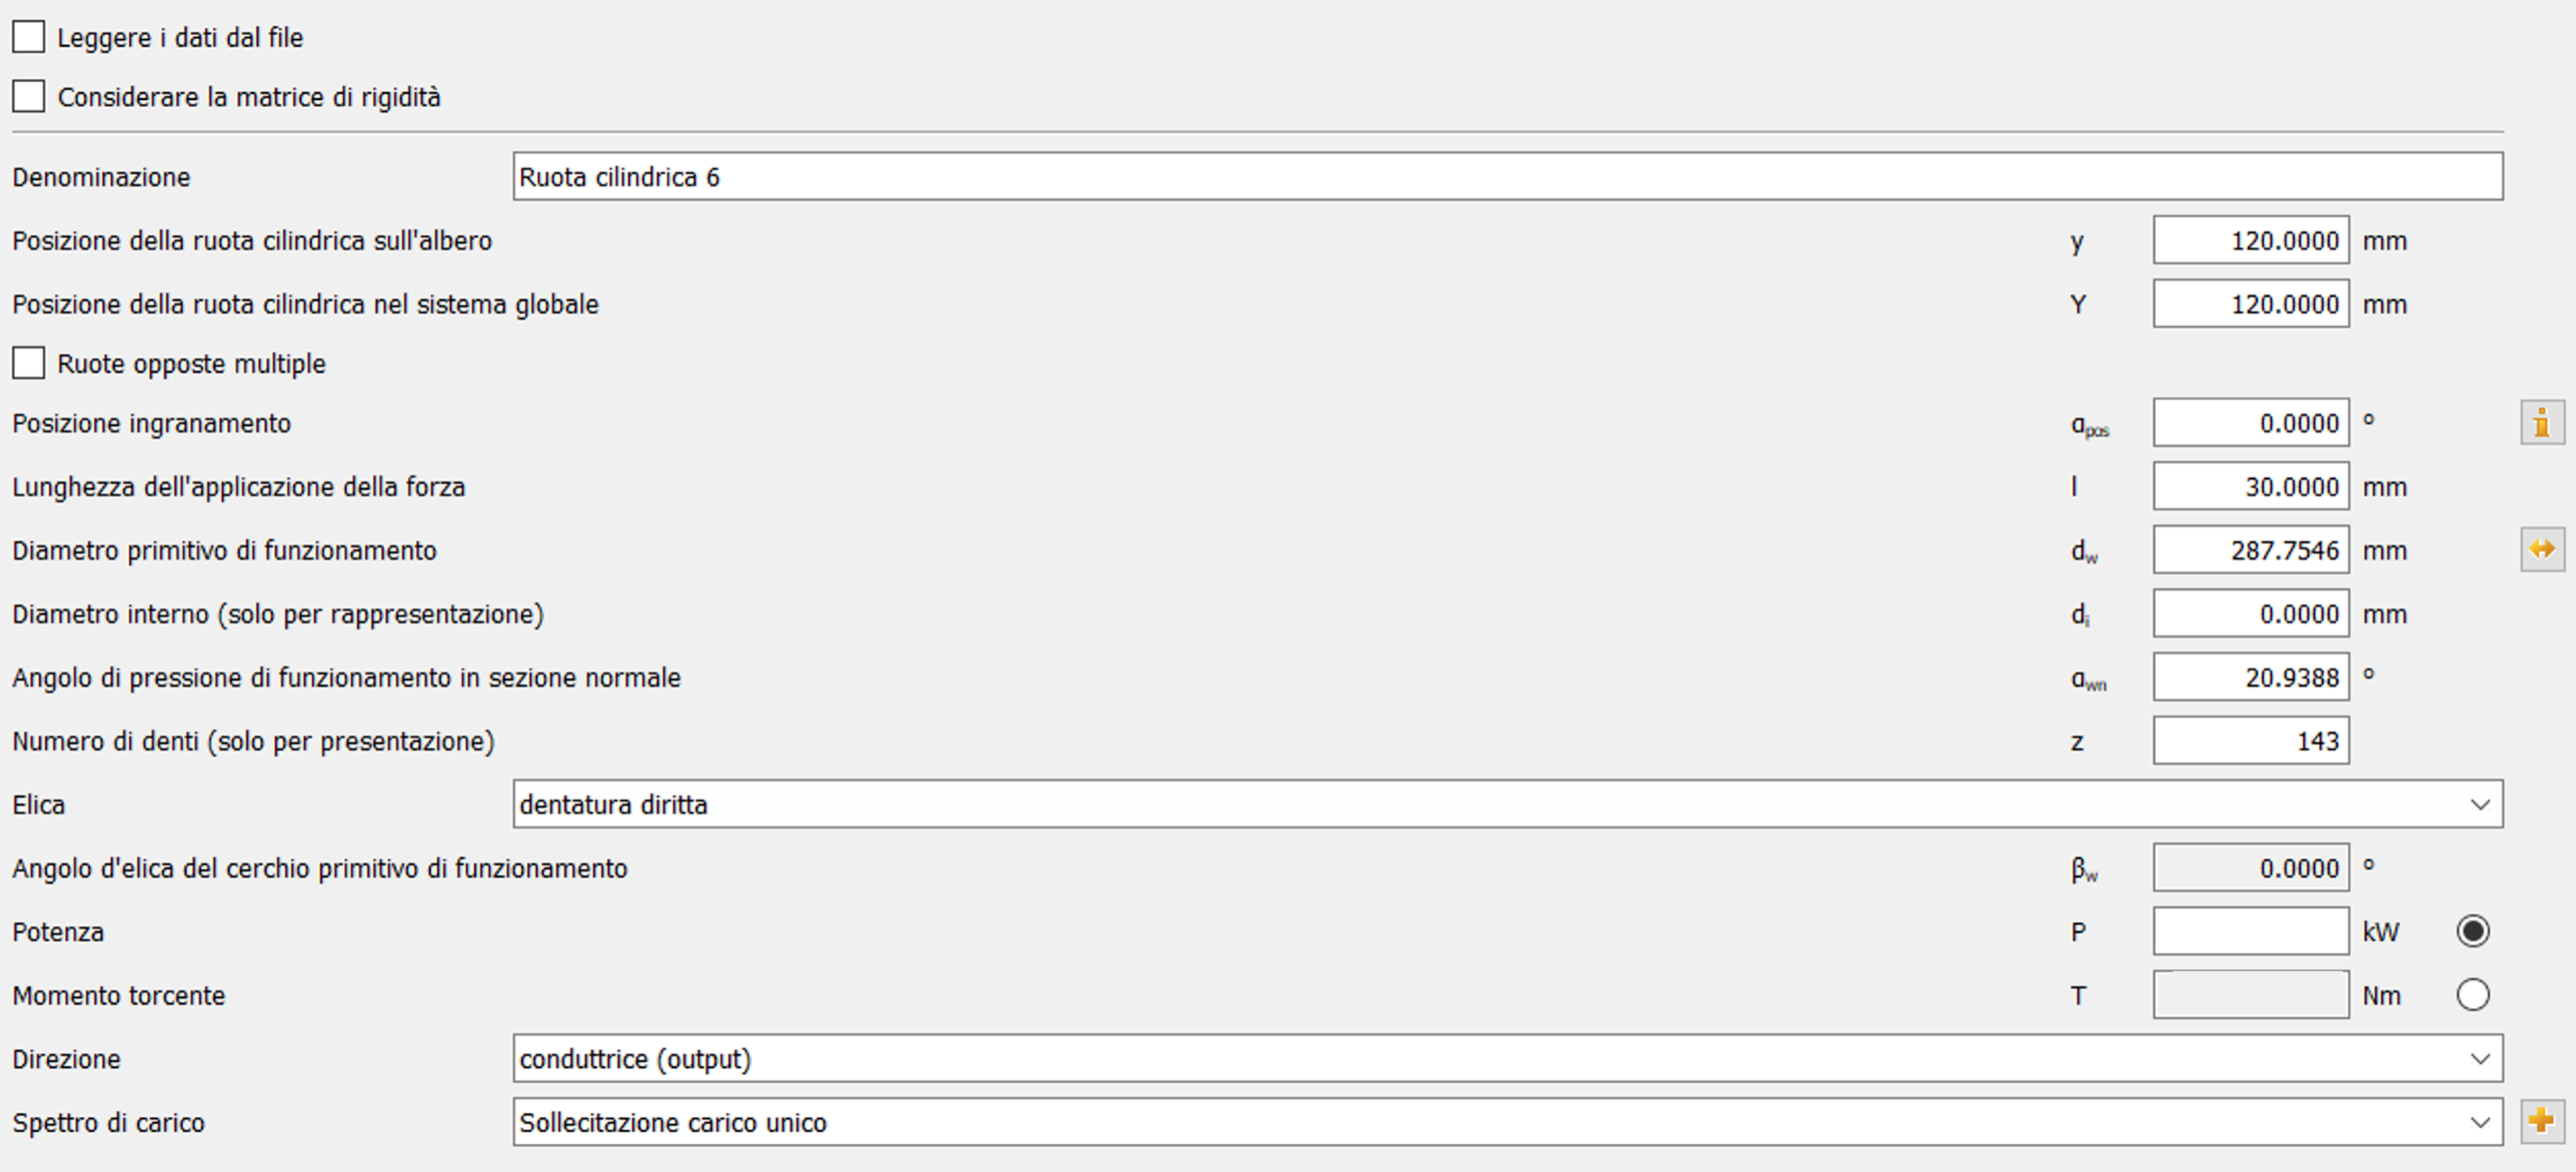
\includegraphics[scale=0.27]{Immagini/Ruota6Albero3.png}
    \caption{Dati delle ruote in output calettate sull'albero 3}
    \label{fig:Ruota1Albero2}
\end{figure}

\newpage
Sono state poi considerate le grandezze di dettaglio:
\begin{figure}[h]
    \centering
    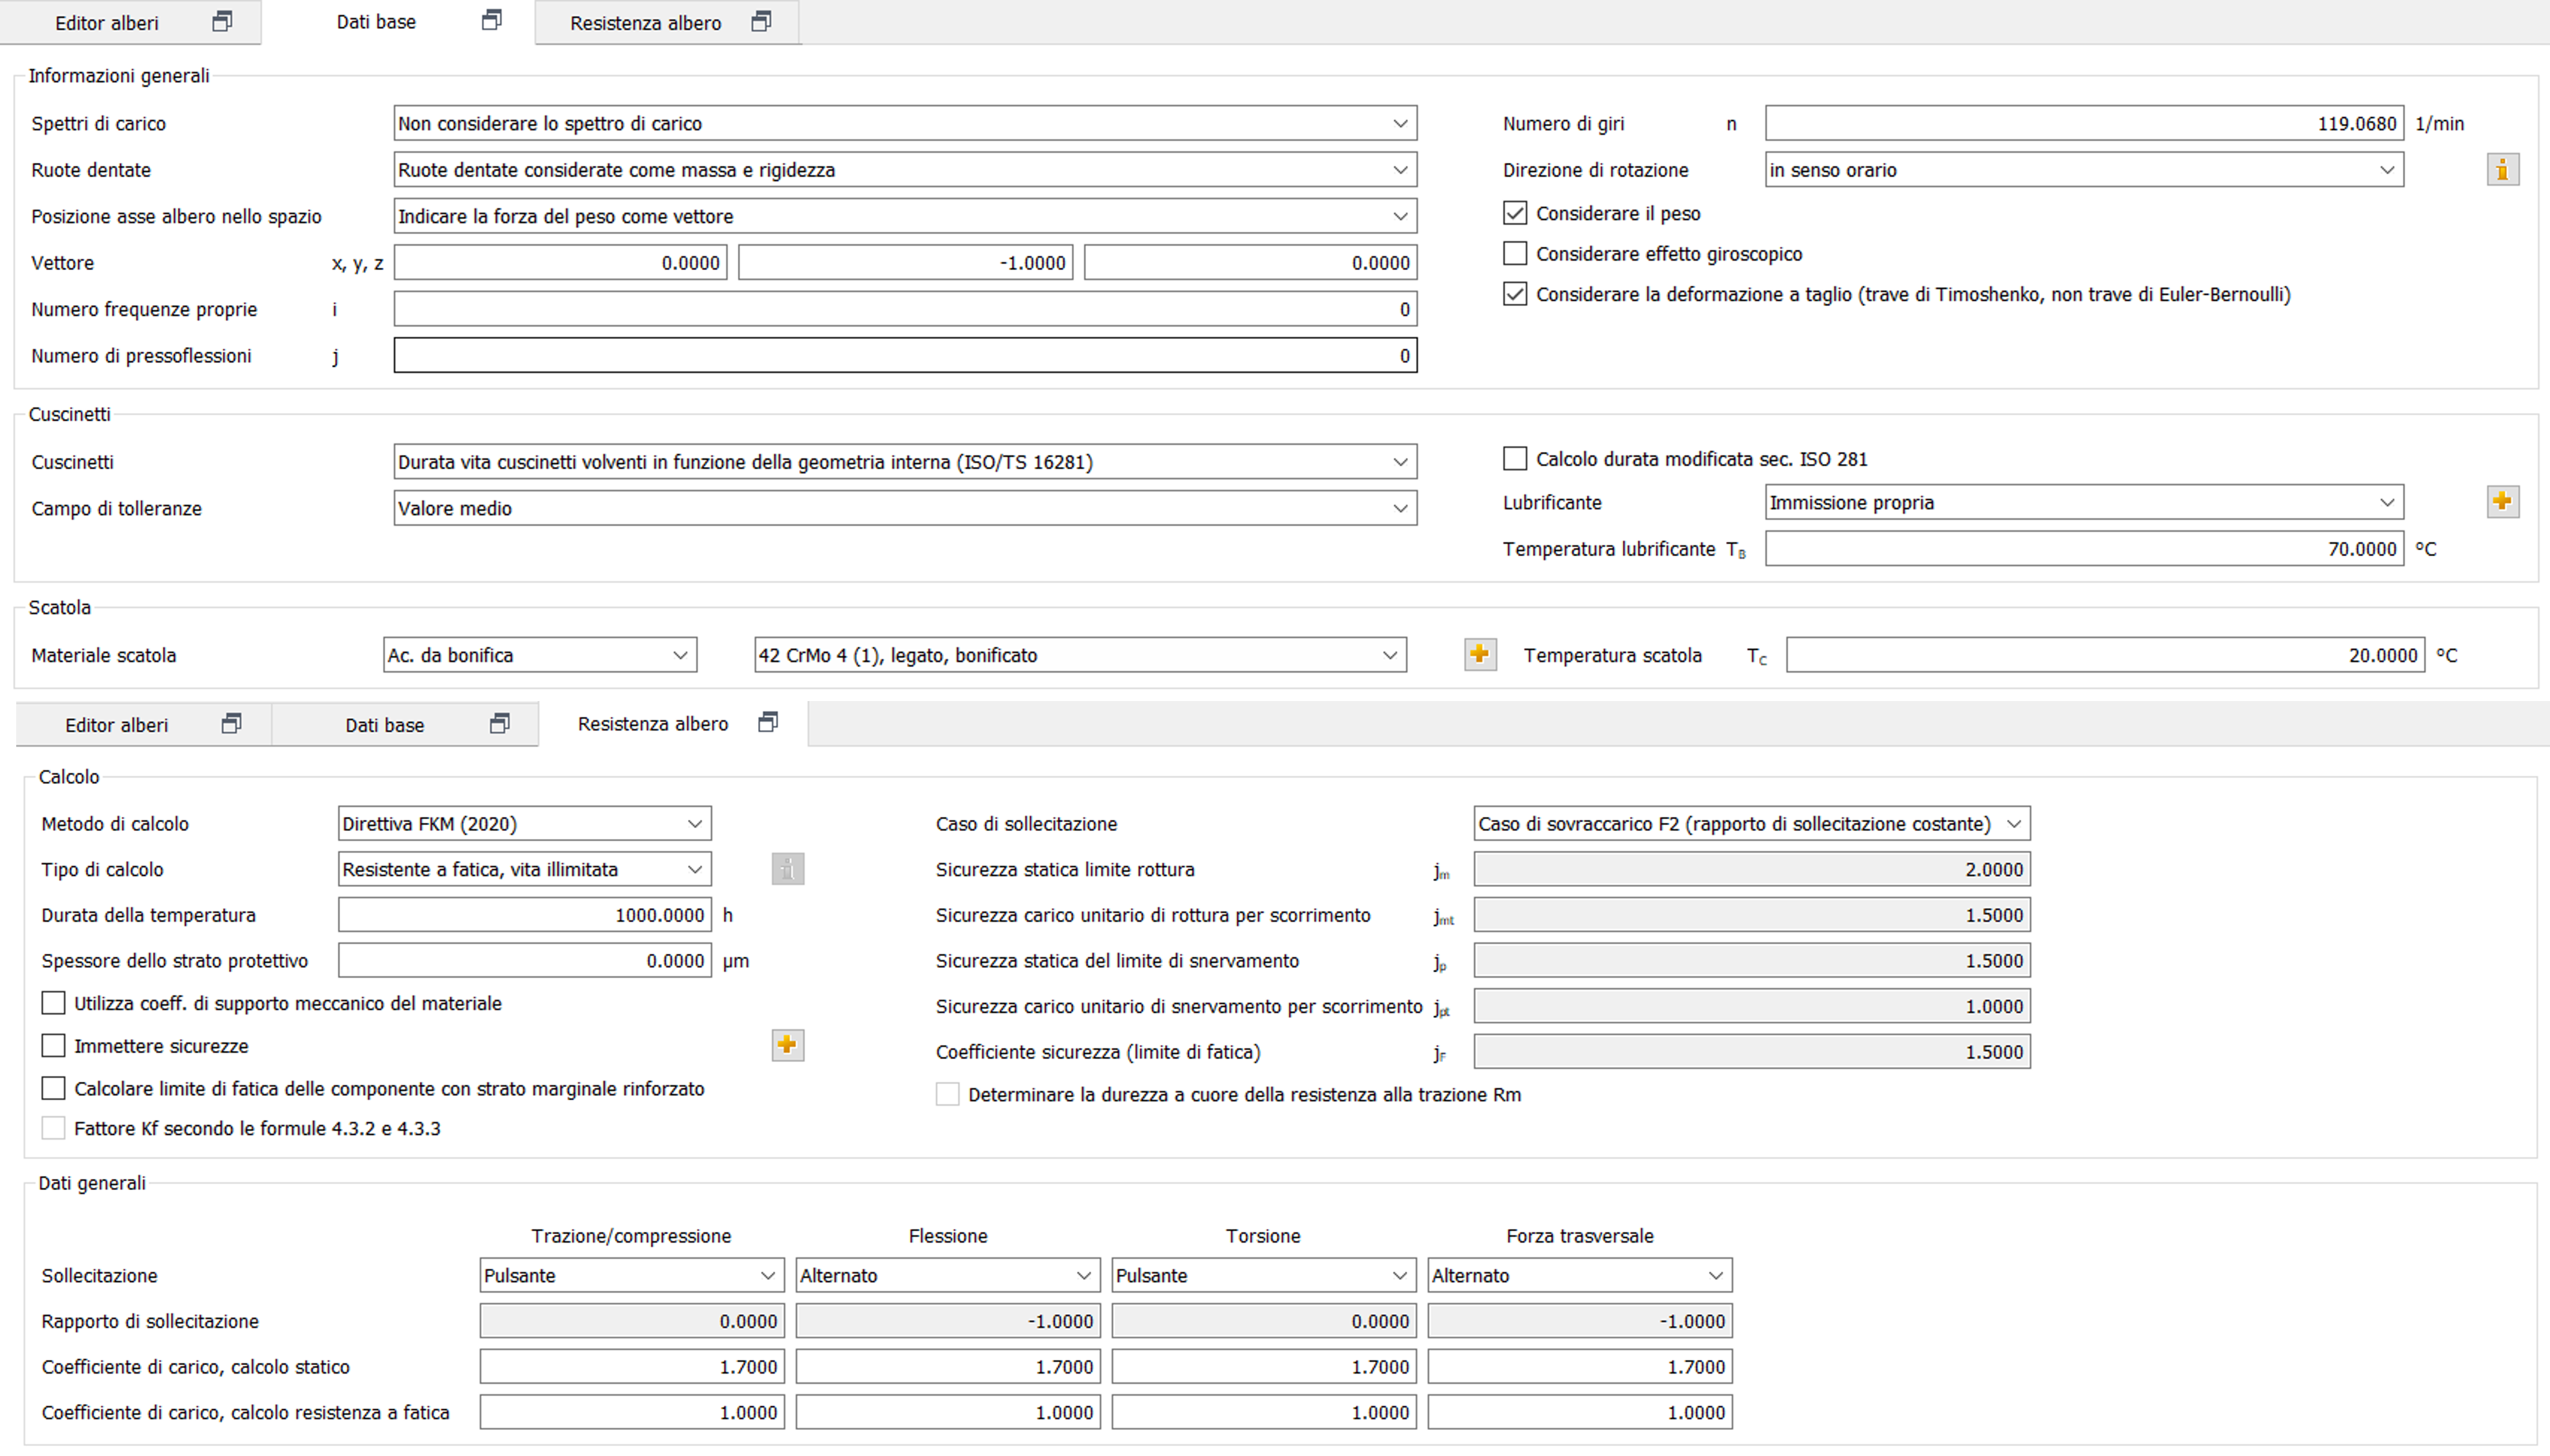
\includegraphics[scale=0.45]{Immagini/DettagliAlbero3.png}
    \caption{Grandezze di dettaglio relative all'analisi dell'albero 3}
    \label{fig:DettagliAlbero3}
\end{figure}

Per analizzare il funzionamento dell'albero 3 è stato necessario osservare tre differenti possibili configurazioni di caricamento in funzione del duty cicle fornito dalla consegna. Questo perché l'albero 3 è l'elemento che pone in collegamento l'input ad entrambi gli output.
\begin{figure}[h]
    \centering
    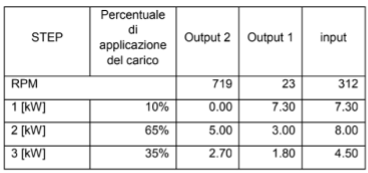
\includegraphics[scale=0.6]{Immagini/Carico.png}
    \caption{Ciclo di carico a cui è sottoposto il riduttore}
    \label{fig:Carico}
\end{figure}

Mentre per le ruote degli altri alberi il valore di potenza risultava univoco, per le ruote dell'albero 3 questa dipende dal ciclo di carico considerato. Durante l'analisi le tre configurazioni sono state denominate:
\begin{itemize}
    \item Step 1;
    \item Step 2;
    \item Step 3.
\end{itemize}

Si procede quindi all'analisi di ciascun step di funzionamento.
\newpage
\textbf{Step 1}
In questa configurazione i dati assunti dagli elementi coinvolti durante il funzionamento dell'albero sono:
\begin{itemize}
    \item Potenza assorbita ruota 3 pari a 7.3 kW;
    \item Potenza erogata ruota 4 (output 1) pari a 7.3 kW;
    \item Potenza assorbita ruota 6 (output 2) pari a 0 kW;
\end{itemize}

Dal Report fornito dal software è possibile ottenere ulteriori informazioni di interesse sull'albero appena progettato. 

\emph{Applicazione del carico}
\begin{figure}[h]
    \centering
    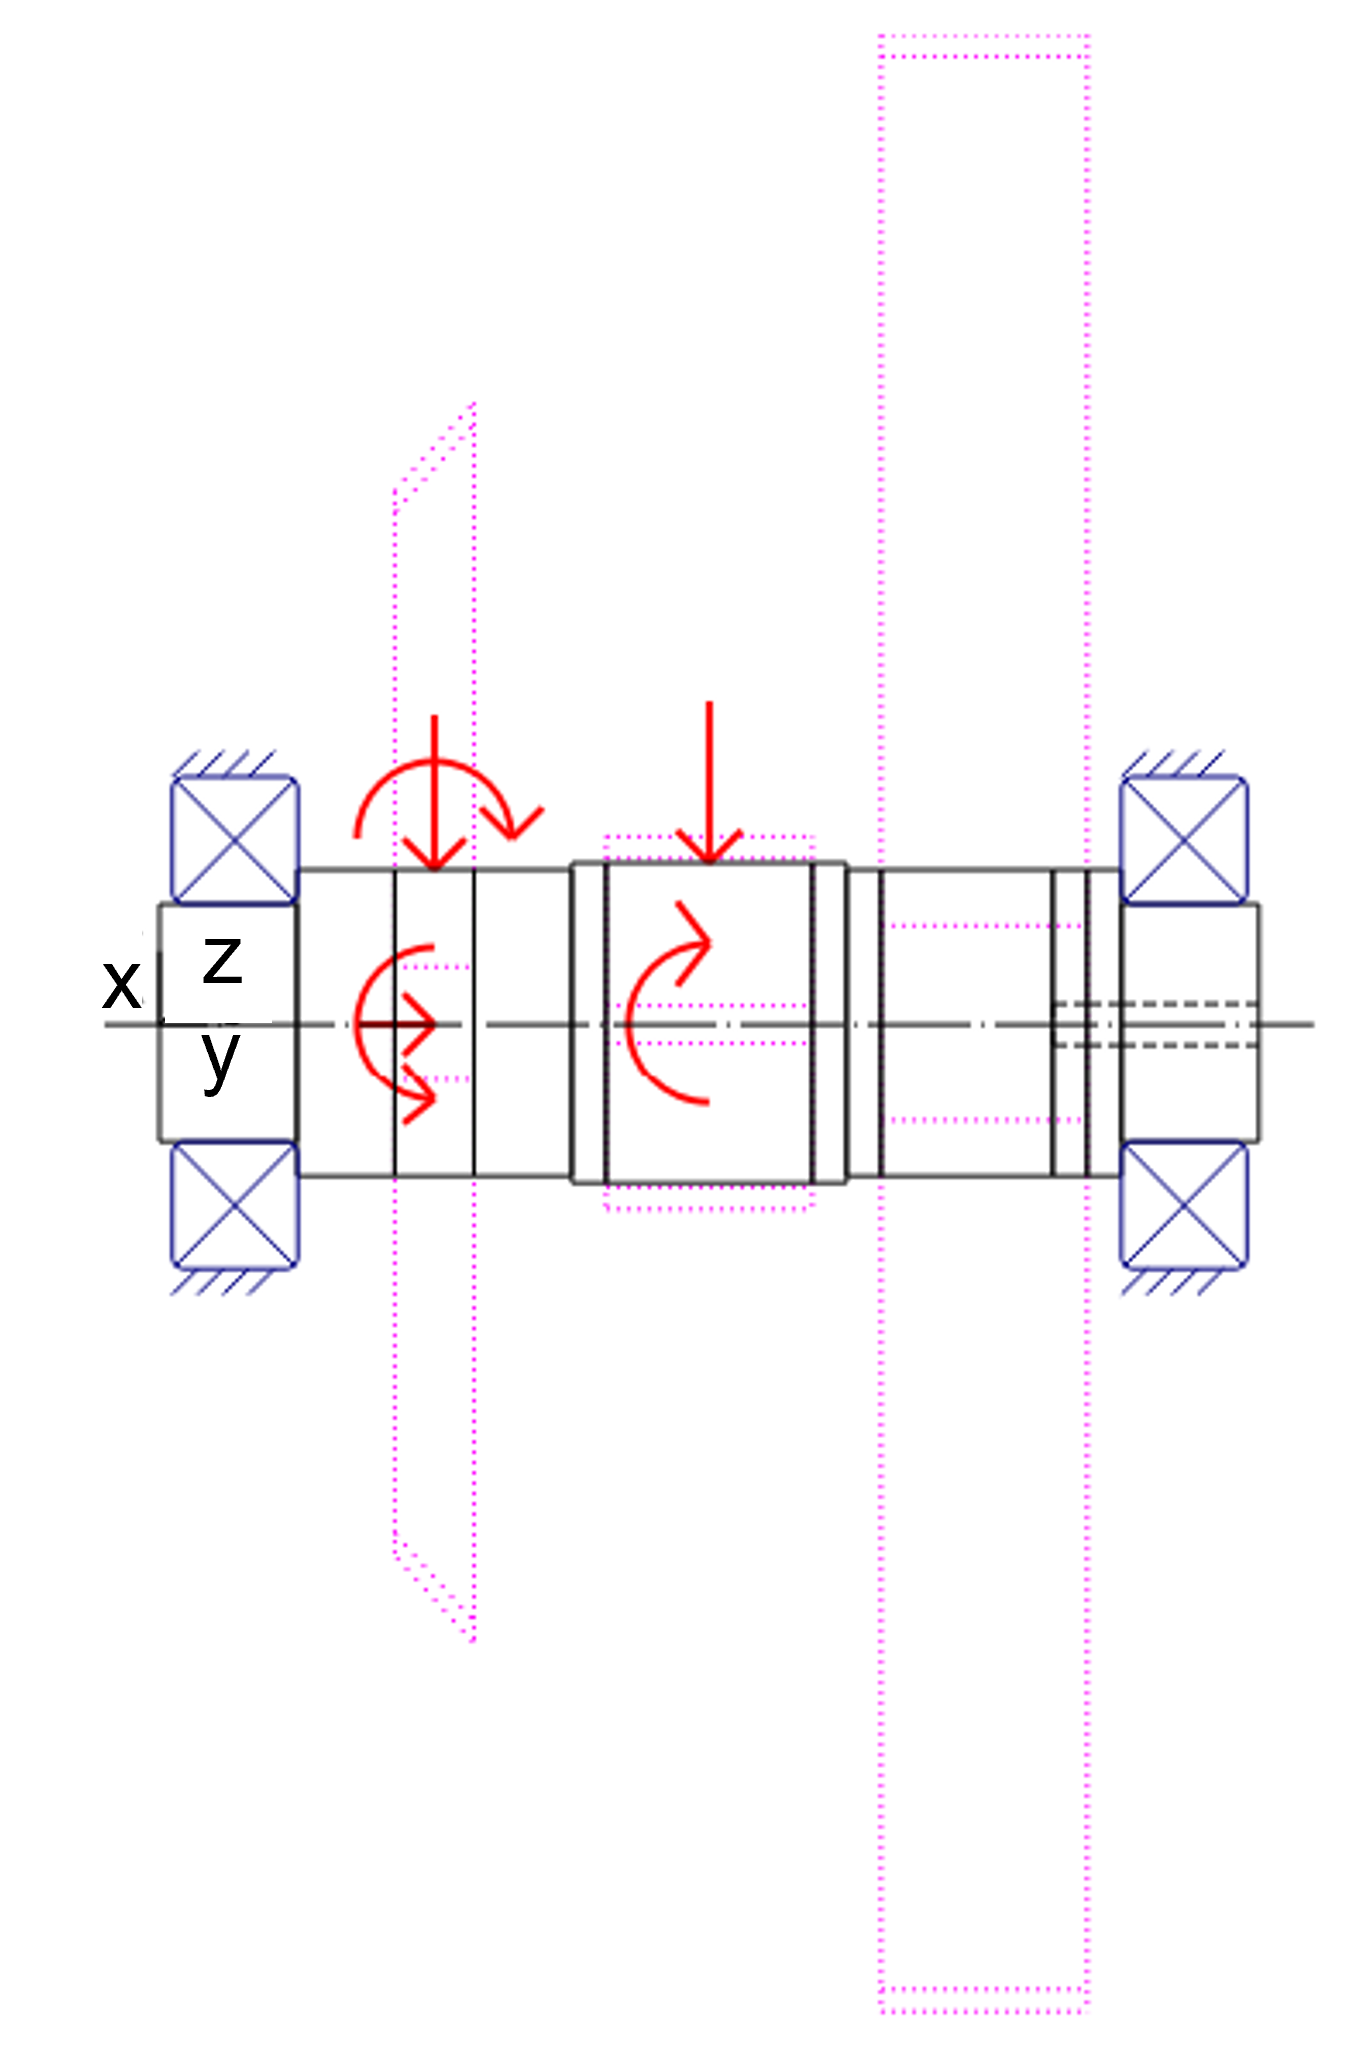
\includegraphics[scale=0.5]{Immagini/Carico1Albero3.png}
    \caption{Applicazione del carico lungo l'albero 3}
    \label{fig:Carico1Albero3}
\end{figure}
\newpage
\emph{Forze agenti sulle ruote}
\begin{figure}[h]
    \centering
    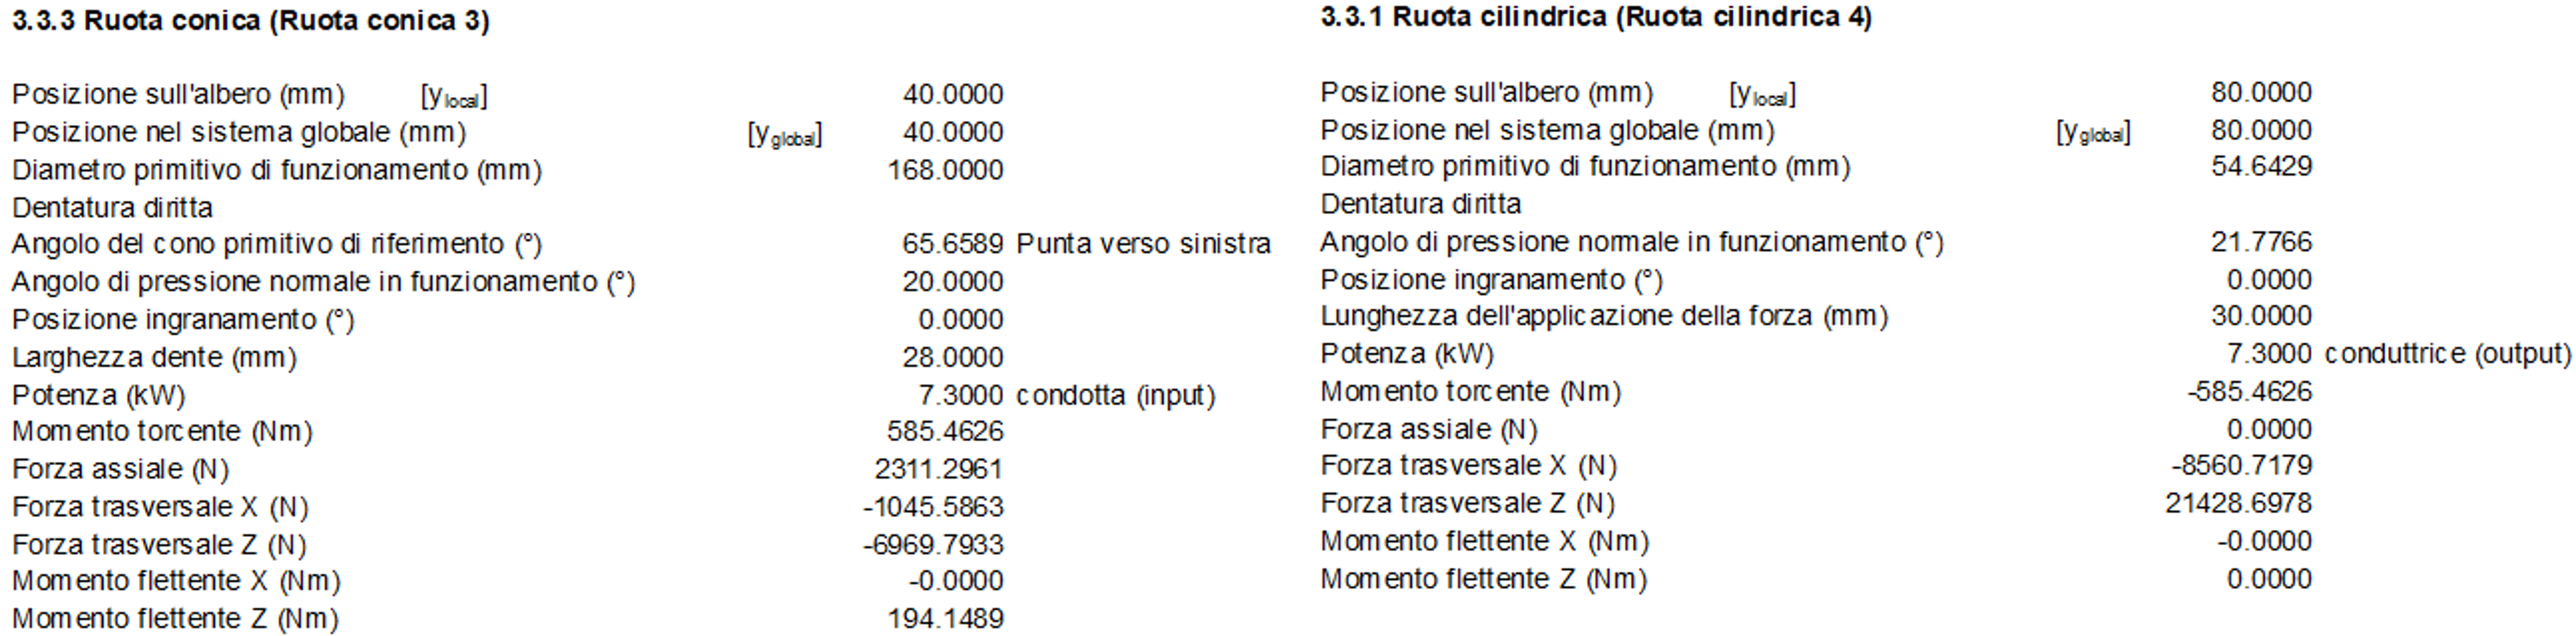
\includegraphics[scale=0.5]{Immagini/Forze1RuoteAlbero3.png}
    \caption{Valore delle forze trasmesse sull'albero 3}
    \label{fig:Forze1RuoteAlbero3}
\end{figure}

\emph{Dettagli cuscinetti}
\begin{figure}[h]
    \centering
    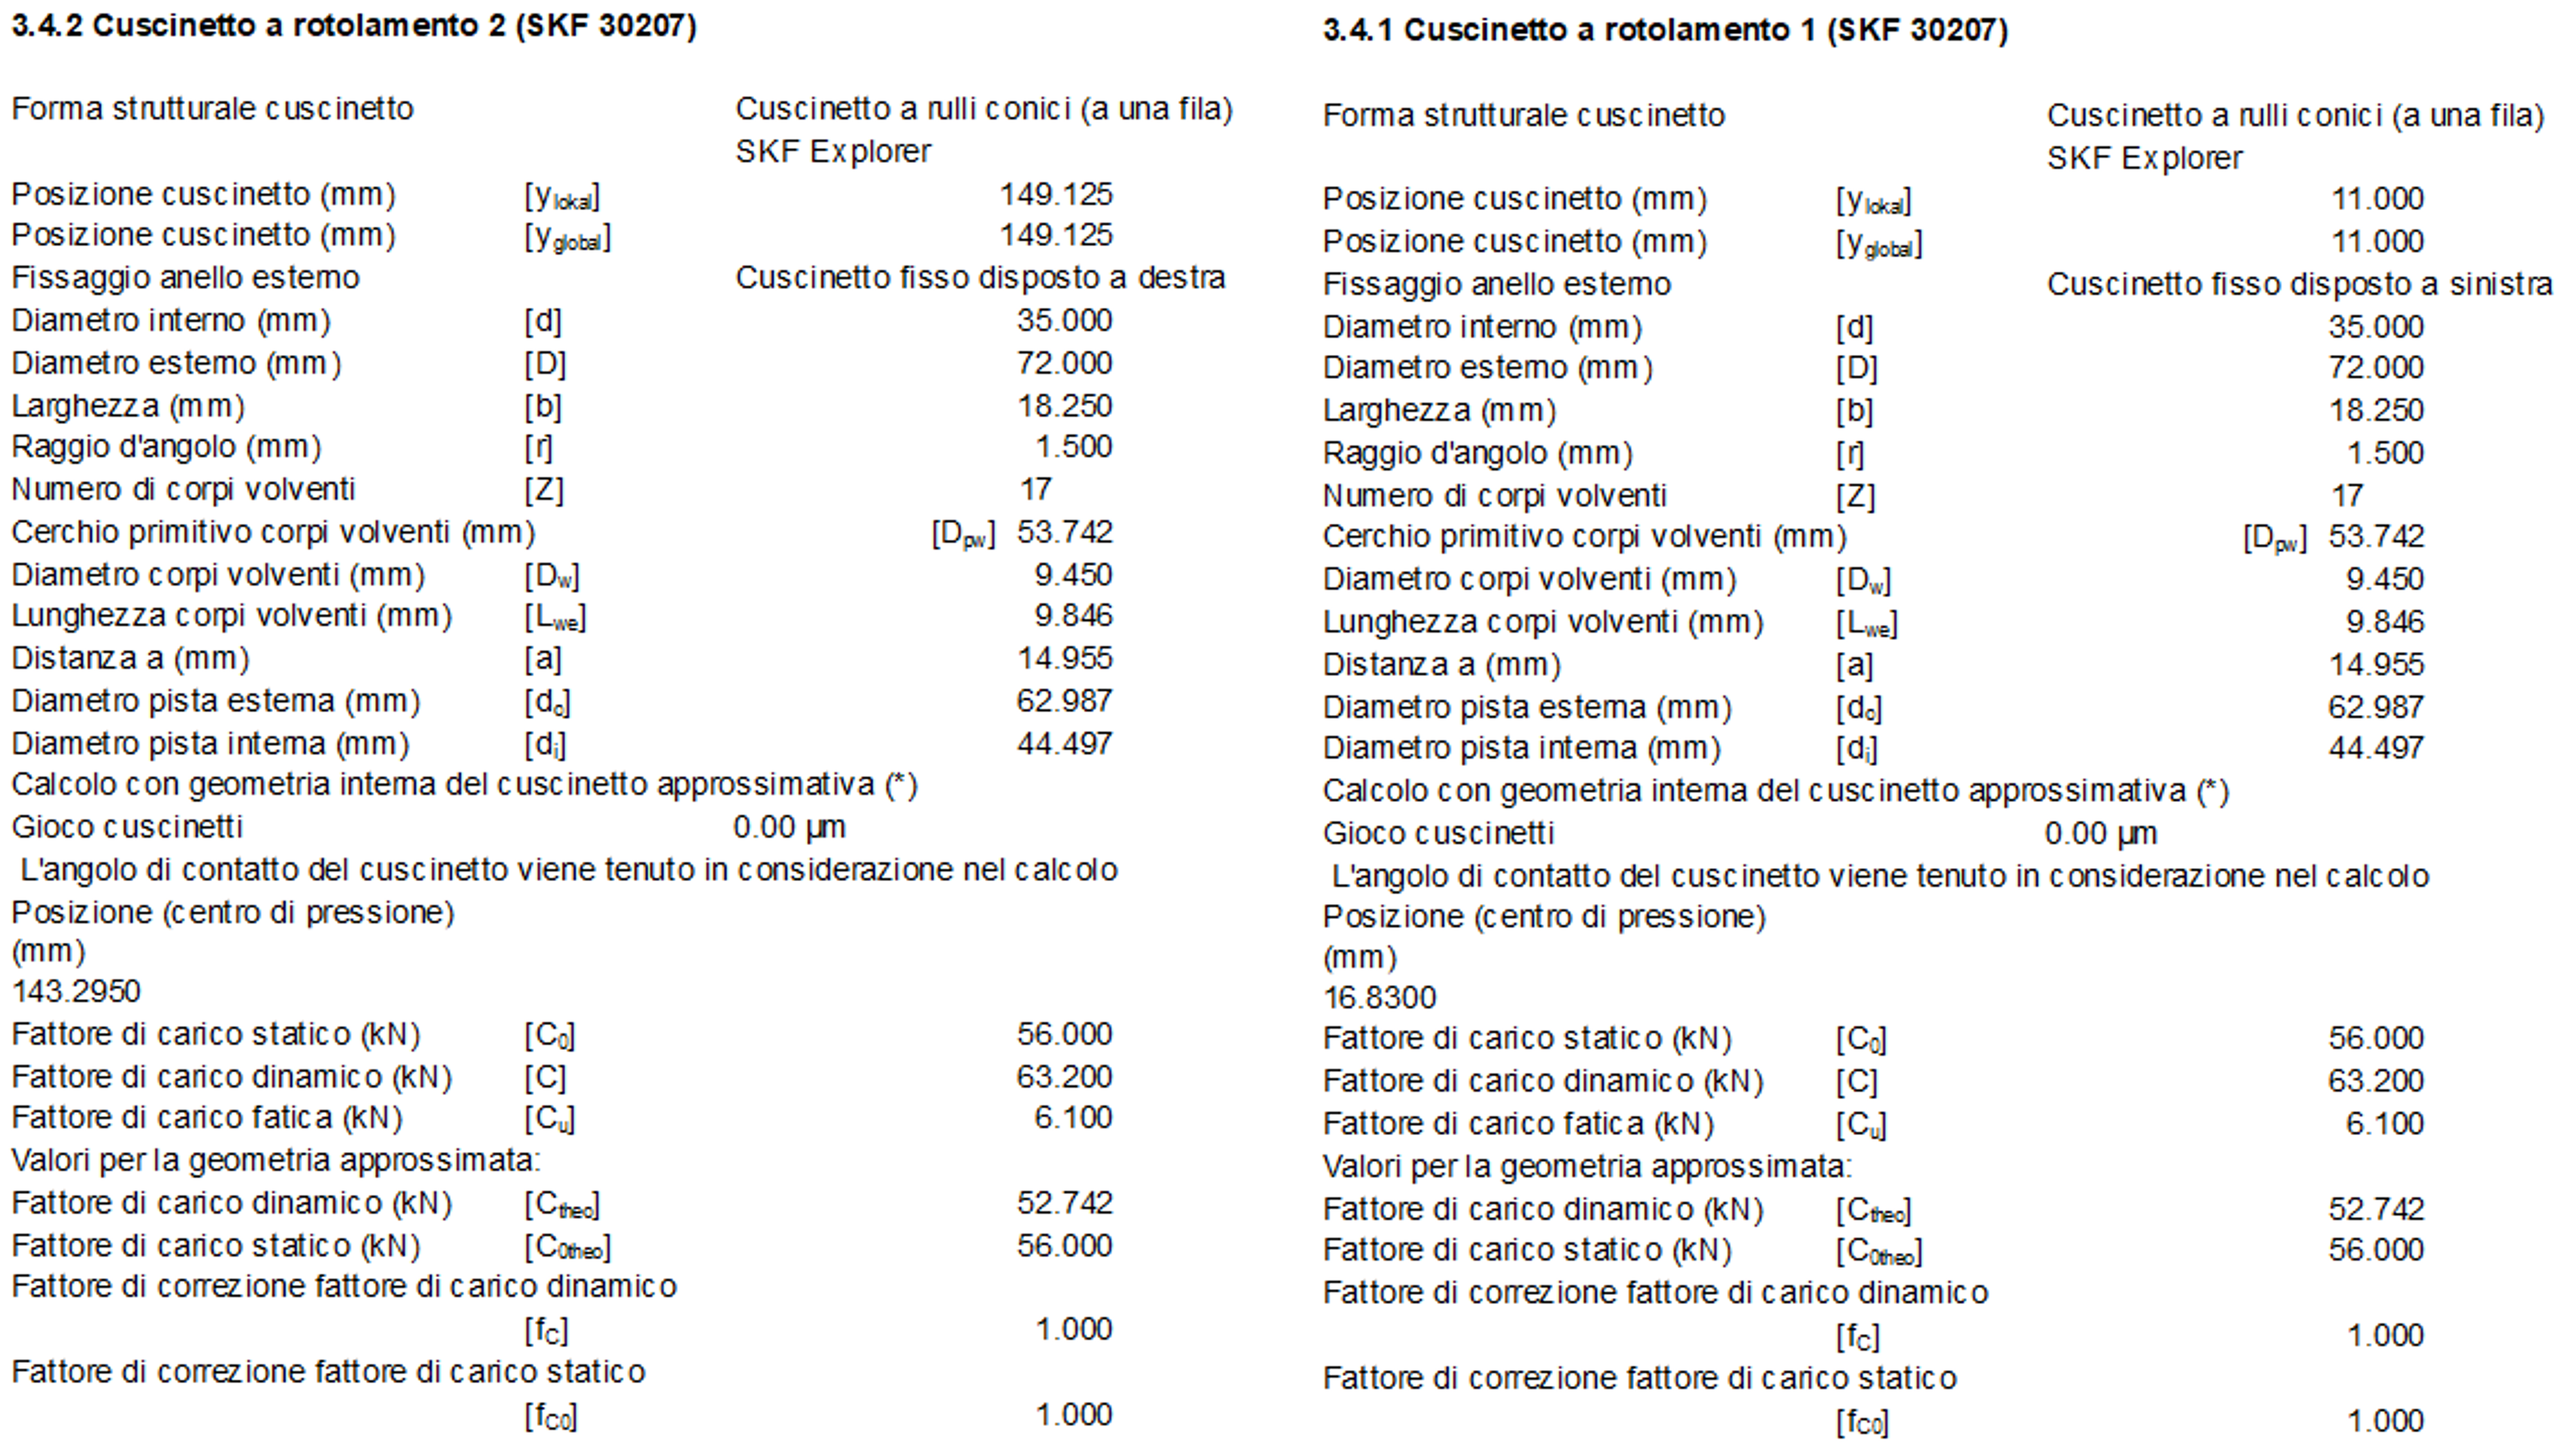
\includegraphics[scale=0.5]{Immagini/Forze1CuscinettiAlbero3.png}
    \caption{Valore delle forze trasmesse sull'albero 3}
    \label{fig:Forze1CusinettiAlbero3}
\end{figure}
\newpage
\emph{Deformazione dell'albero}
\begin{figure}[h]
    \centering
    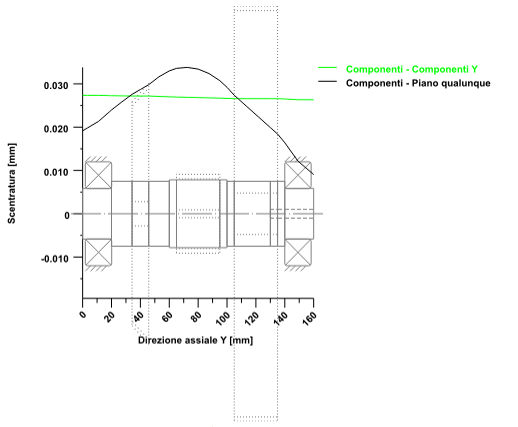
\includegraphics[scale=0.5]{Immagini/Deformata1Albero3.png}
    \caption{Deformata dell'albero 3}
    \label{fig:Deformata1Albero3}
\end{figure}

\emph{Andamento della tensione equivalente}
\begin{figure}[h]
    \centering
    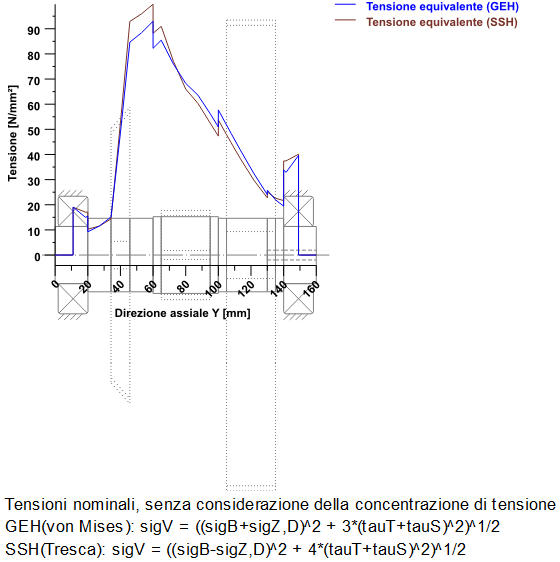
\includegraphics[scale=0.5]{Immagini/Tensioni1Albero3.png}
    \caption{Andamento della tensione equivalente lungo l'albero 3}
    \label{fig:Tensioni1Albero3}
\end{figure}
\newpage
Infine, attraverso la compilazione del software si è osservato come tutte le sezioni fossero ampiamente verificate sia staticamente che a fatica.
\begin{figure}[h]
    \centering
    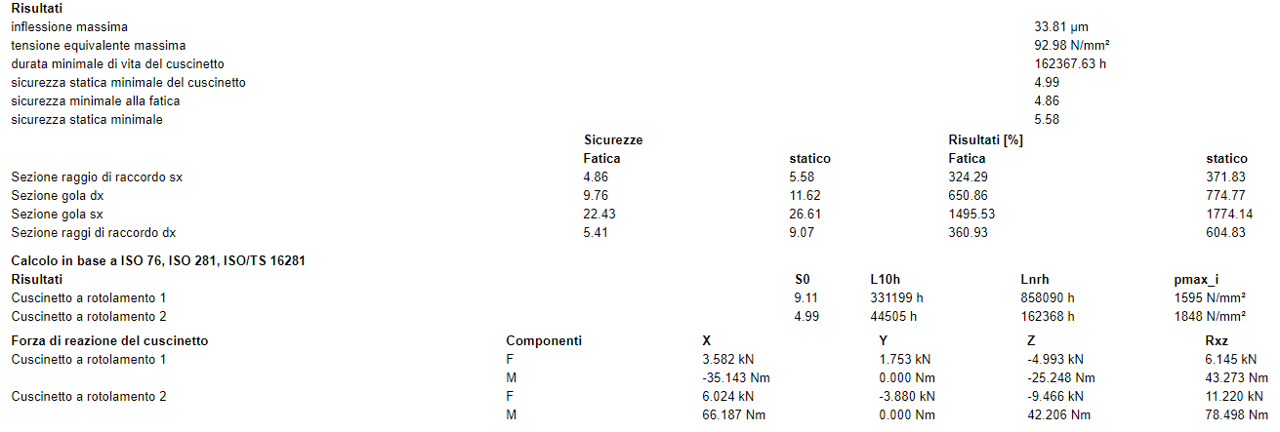
\includegraphics[scale=0.4]{Immagini/Risultati1Albero3.png}
    \caption{Risultato dell'analisi statica e a fatica delle sezioni di interesse dell'albero 3}
    \label{fig:Risultati1Albero3}
\end{figure}

\textbf{Step 2}
In questa configurazione i dati assunti dagli elementi coinvolti durante il funzionamento dell'albero sono:
\begin{itemize}
    \item Potenza assorbita ruota 3 pari a 8 kW;
    \item Potenza erogata ruota 4 (output 1) pari a 3 kW;
    \item Potenza assorbita ruota 6 (output 2) pari a 5 kW;
\end{itemize}

Dal Report fornito dal software è possibile ottenere ulteriori informazioni di interesse sull'albero appena progettato. 

\emph{Applicazione del carico}
\begin{figure}[h]
    \centering
    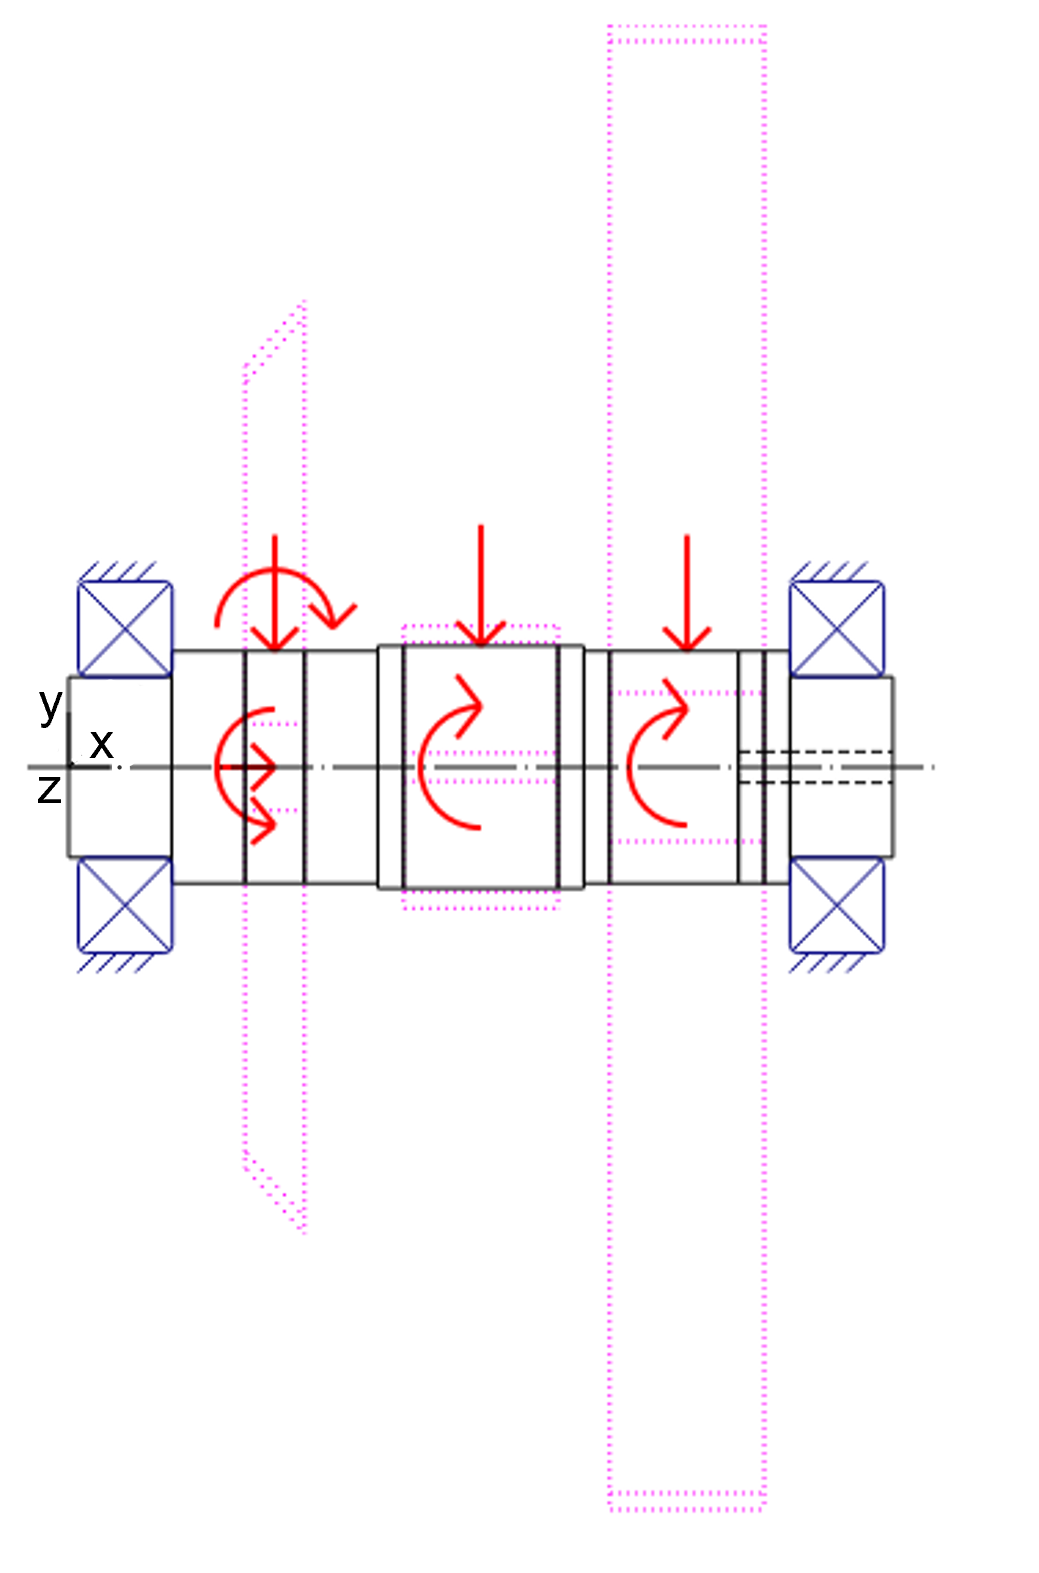
\includegraphics[scale=0.5]{Immagini/Carico2Albero3.png}
    \caption{Applicazione del carico lungo l'albero 3}
    \label{fig:Carico2Albero3}
\end{figure}
\newpage
\emph{Forze agenti sulle ruote}
\begin{figure}[h]
    \centering
    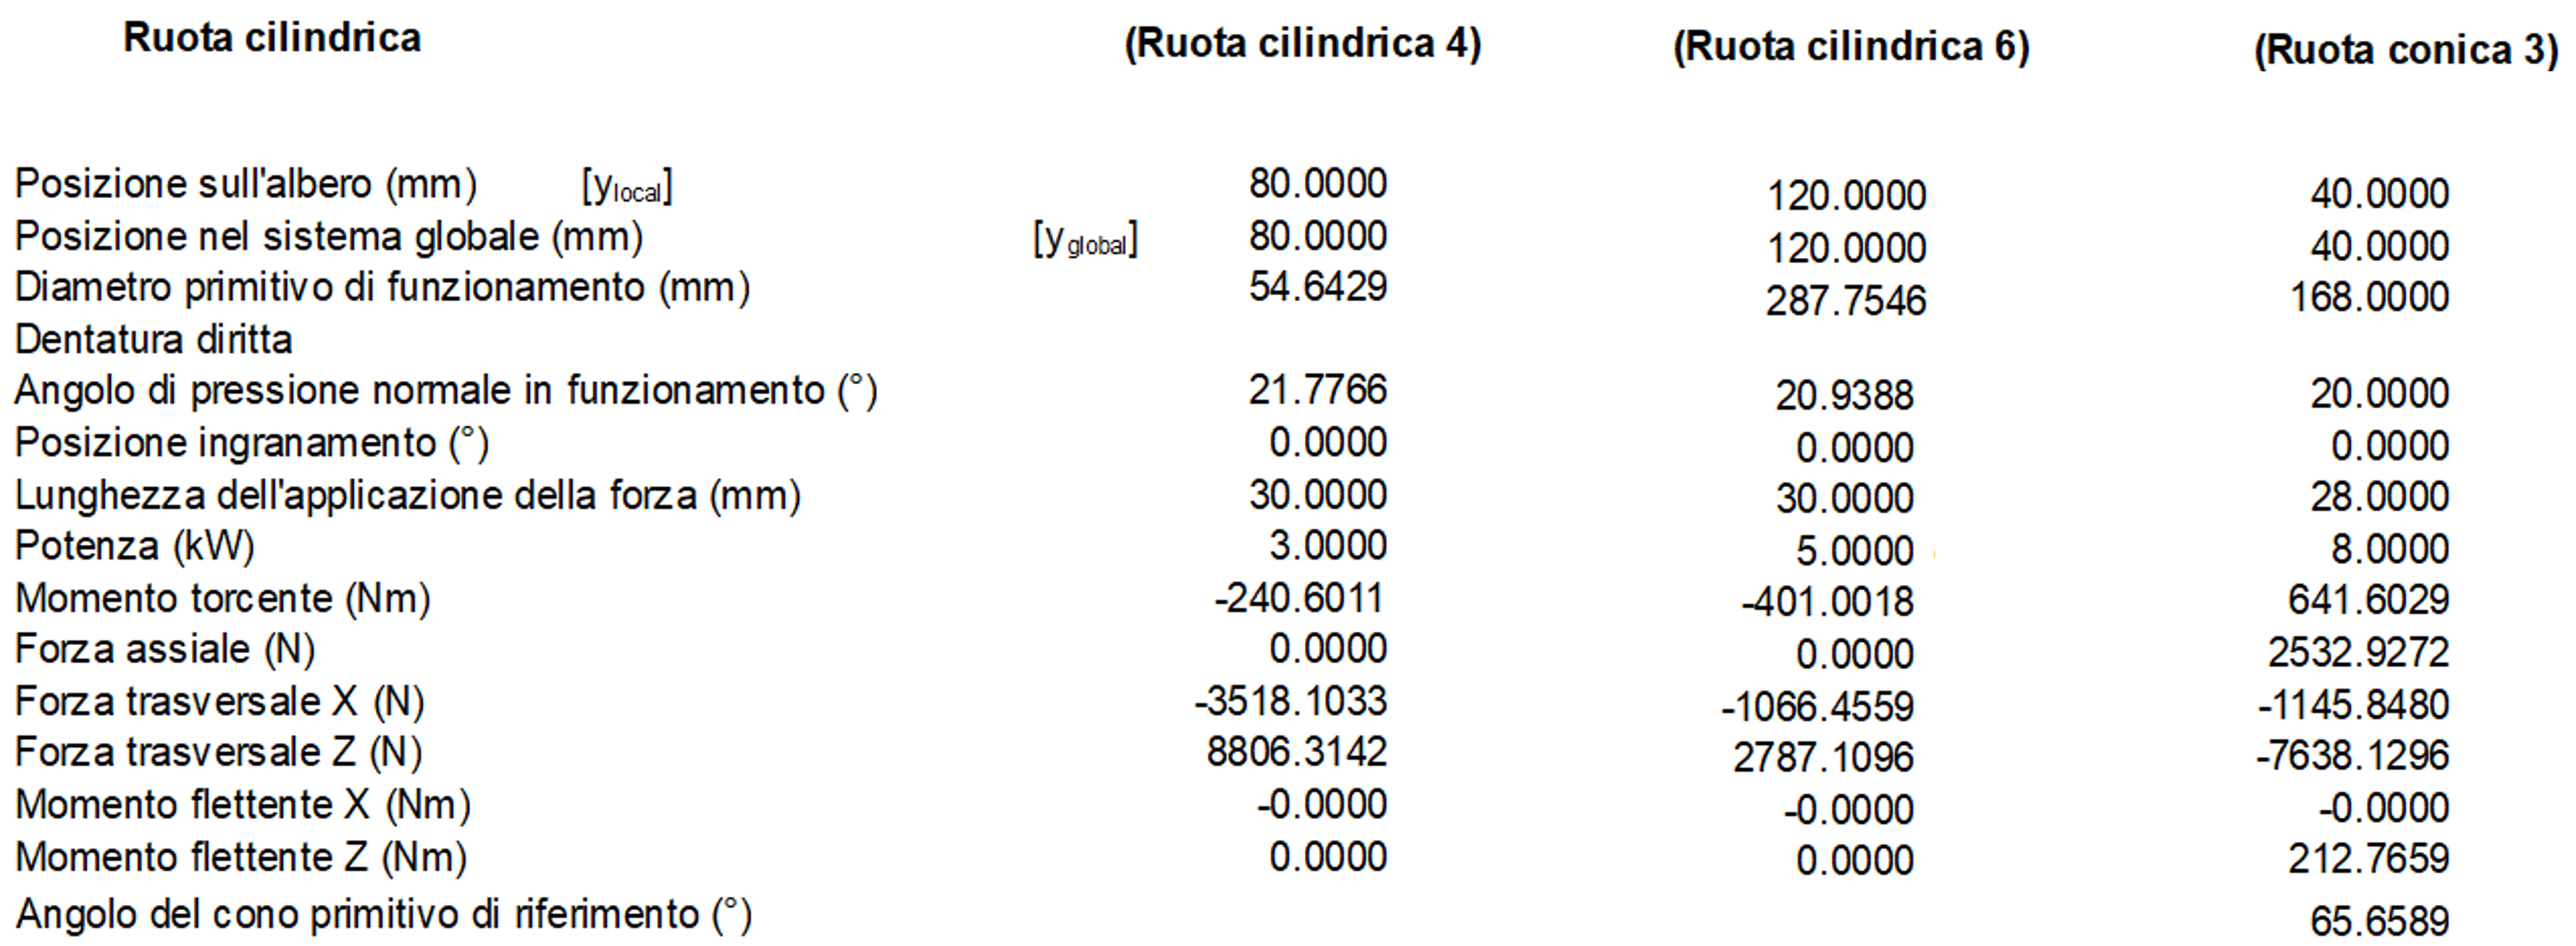
\includegraphics[scale=0.5]{Immagini/Forze2RuoteAlbero3.png}
    \caption{Valore delle forze trasmesse sull'albero 3}
    \label{fig:Forze2RuoteAlbero3}
\end{figure}

\emph{Dettagli cuscinetti}
\begin{figure}[h]
    \centering
    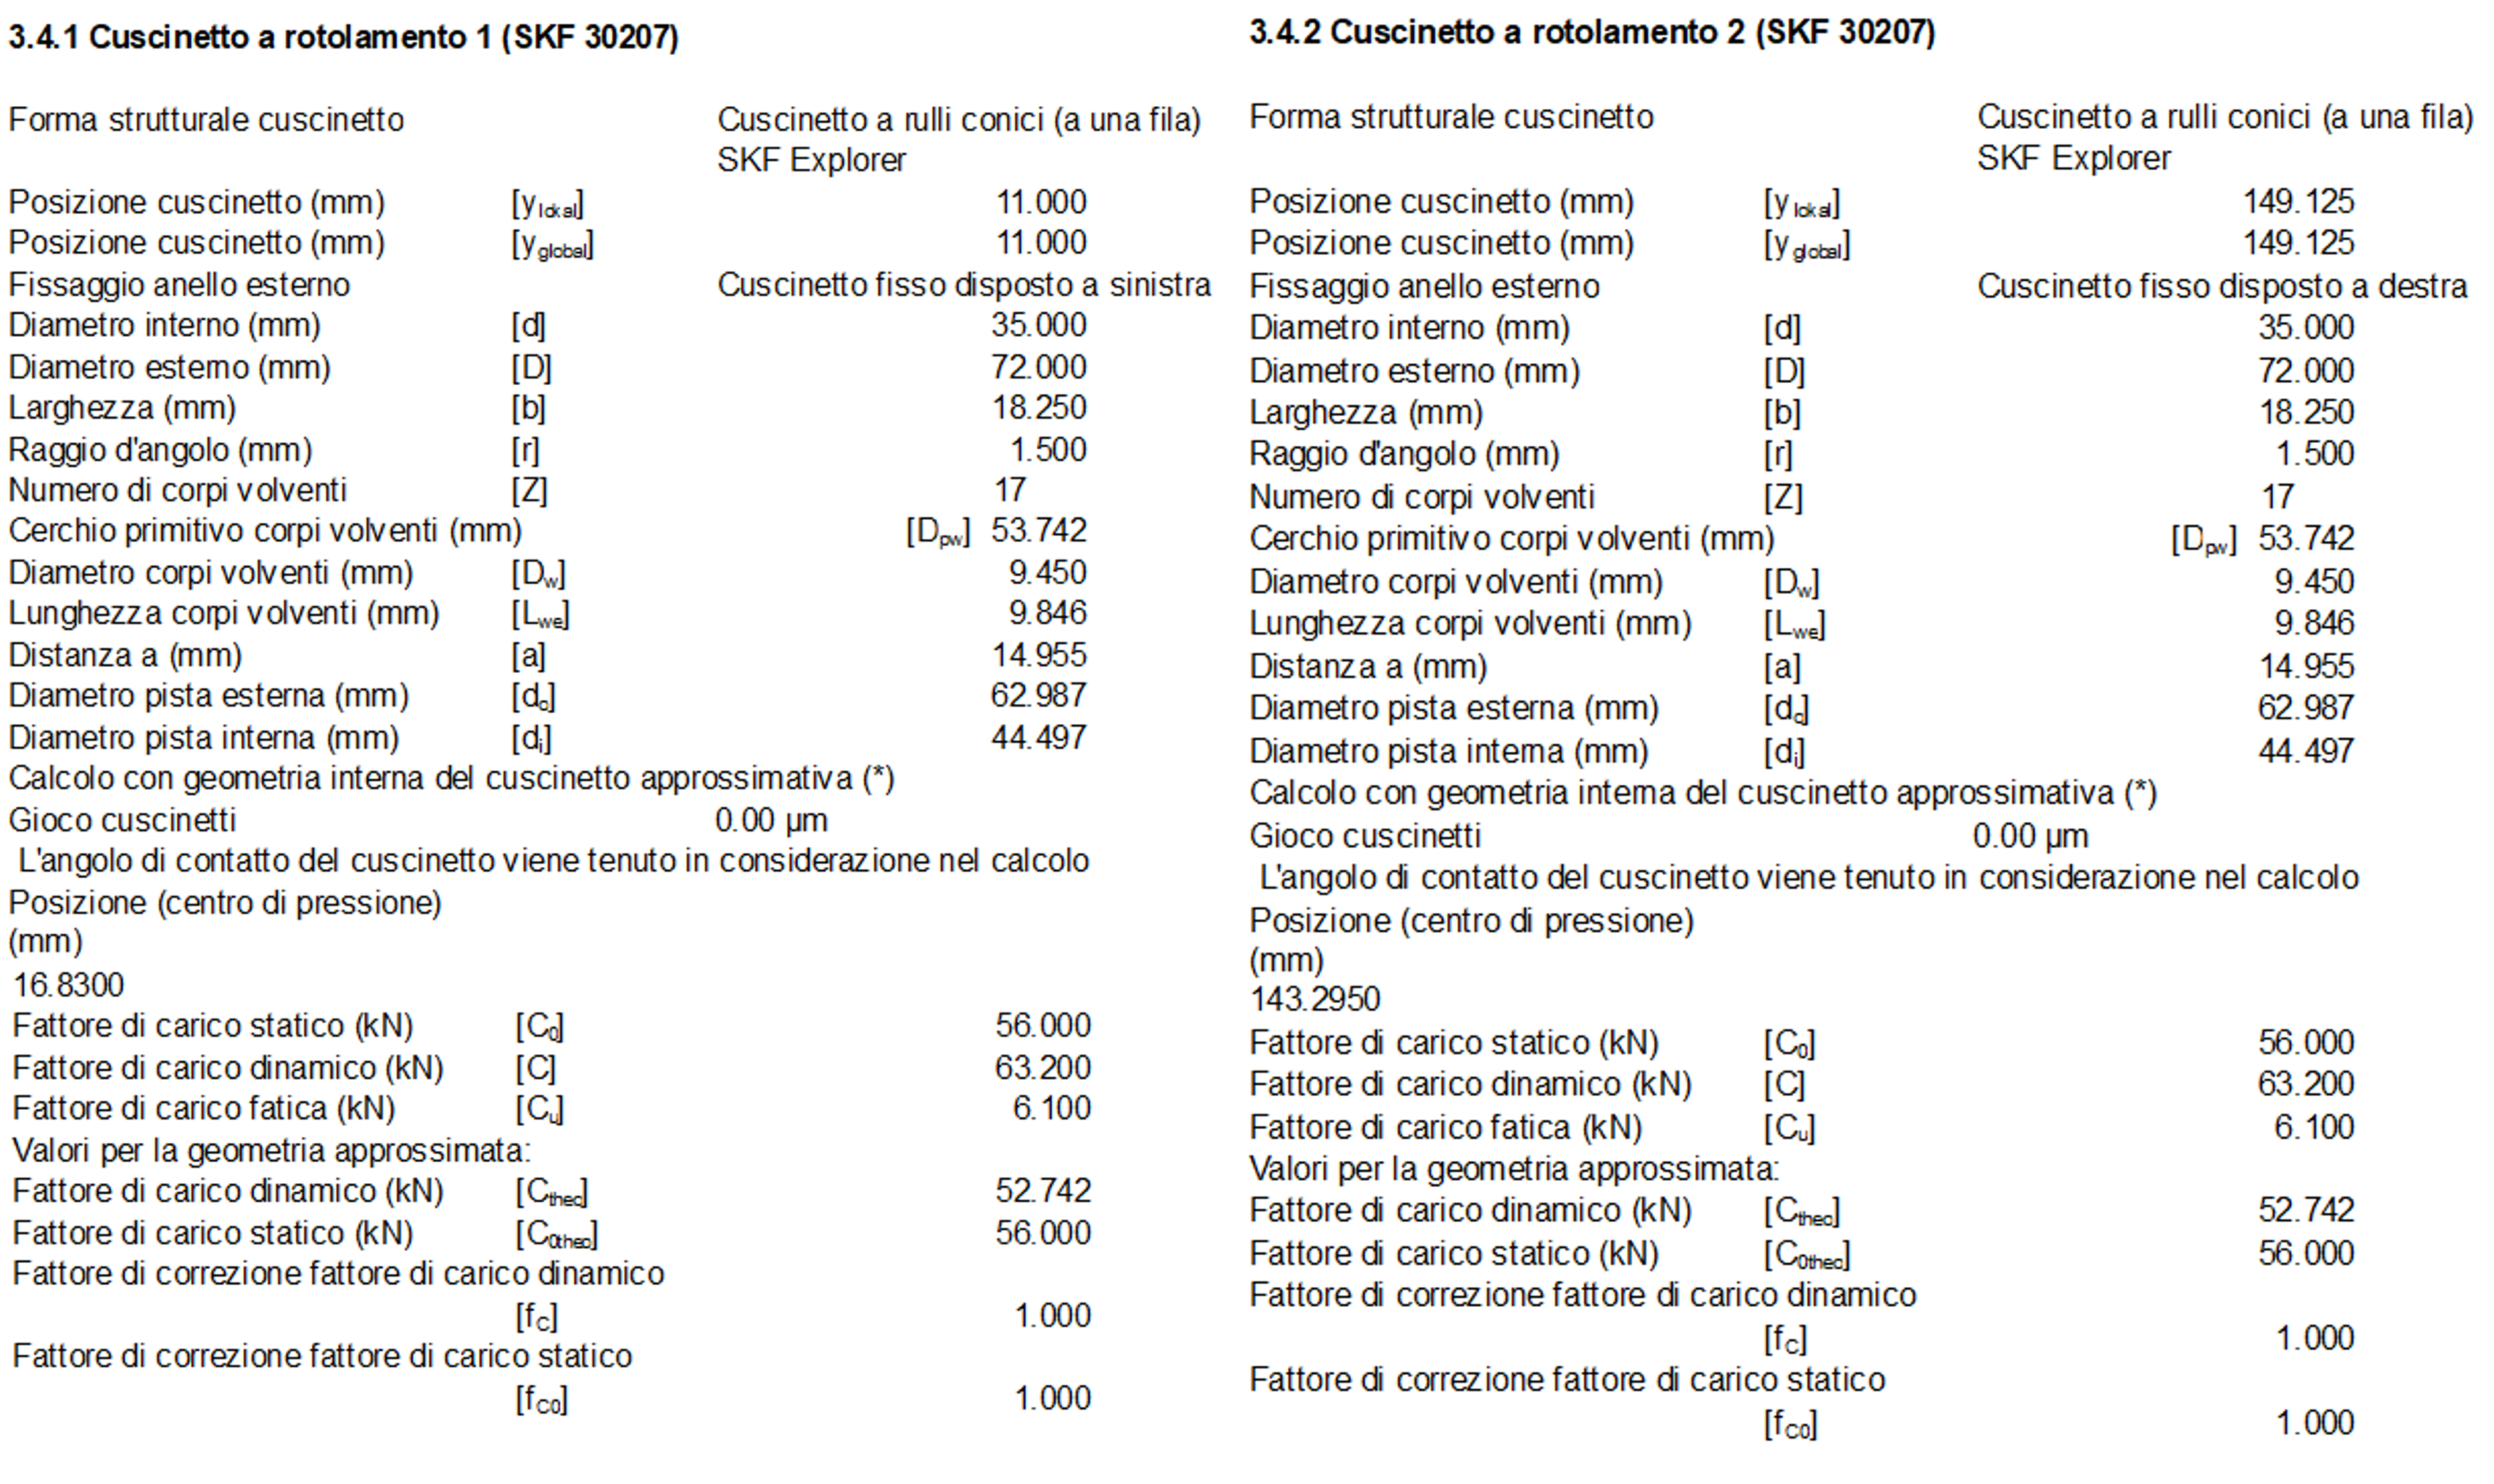
\includegraphics[scale=0.5]{Immagini/Forze2CuscinettiAlbero3.png}
    \caption{Valore delle forze trasmesse sull'albero 3}
    \label{fig:Forze2CusinettiAlbero3}
\end{figure}
\newpage
\emph{Deformazione dell'albero}
\begin{figure}[h]
    \centering
    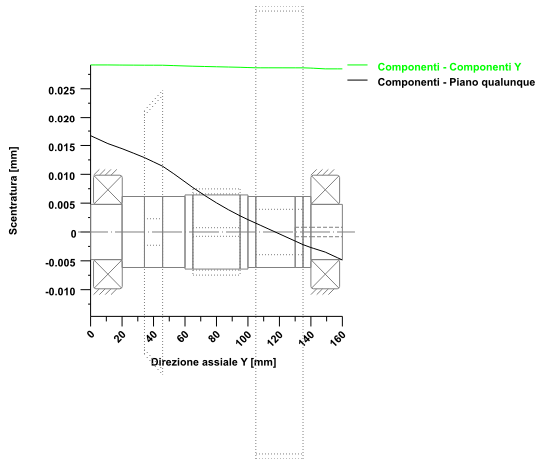
\includegraphics[scale=0.5]{Immagini/Deformata2Albero3.png}
    \caption{Deformata dell'albero 3}
    \label{fig:Deformata2Albero3}
\end{figure}

\emph{Andamento della tensione equivalente}
\begin{figure}[h]
    \centering
    \includegraphics[scale=0.5]{Immagini/Tensioni2Albero3.png}
    \caption{Andamento della tensione equivalente lungo l'albero 3}
   \label{fig:Tensioni2Albero3}
\end{figure}
\newpage
Infine, attraverso la compilazione del software si è osservato come tutte le sezioni fossero ampiamente verificate sia staticamente che a fatica.
\begin{figure}[h]
    \centering
    \includegraphics[scale=0.5]{Immagini/Risultati2Albero3.png}
    \caption{Risultato dell'analisi statica e a fatica delle sezioni di interesse dell'albero 3}
    \label{fig:Risultat21Albero3}
\end{figure}

\textbf{Step 3}
In questa configurazione i dati assunti dagli elementi coinvolti durante il funzionamento dell'albero sono:
\begin{itemize}
    \item Potenza assorbita ruota 3 pari a 4.5 kW;
    \item Potenza erogata ruota 4 (output 1) pari a 1.8 kW;
    \item Potenza assorbita ruota 6 (output 2) pari a 2.7 kW;
\end{itemize}

Dal Report fornito dal software è possibile ottenere ulteriori informazioni di interesse sull'albero appena progettato. 

\emph{Applicazione del carico}
\begin{figure}[h]
    \centering
    \includegraphics[scale=0.5]{Immagini/Carico3Albero3.png}
    \caption{Applicazione del carico lungo l'albero 3}
    \label{fig:Carico3Albero3}
\end{figure}
\newpage
\emph{Forze agenti sulle ruote}
\begin{figure}[h]
    \centering
    \includegraphics[scale=0.5]{Immagini/Forze3RuoteAlbero3.png}
    \caption{Valore delle forze trasmesse sull'albero 3}
    \label{fig:Forze3RuoteAlbero3}
\end{figure}

\emph{Dettagli cuscinetti}
\begin{figure}[h]
    \centering
    \includegraphics[scale=0.5]{Immagini/Forze3CuscinettiAlbero3.png}
    \caption{Valore delle forze trasmesse sull'albero 3}
    \label{fig:Forze3CusinettiAlbero3}
\end{figure}
\newpage
\emph{Deformazione dell'albero}
\begin{figure}[h]
    \centering
    \includegraphics[scale=0.5]{Immagini/Deformata3Albero3.png}
    \caption{Deformata dell'albero 3}
    \label{fig:Deformata3Albero3}
\end{figure}

\emph{Andamento della tensione equivalente}
\begin{figure}[h]
    \centering
    \includegraphics[scale=0.5]{Immagini/Tensioni3Albero3.png}
    \caption{Andamento della tensione equivalente lungo l'albero 3}
   \label{fig:Tensioni3Albero3}
\end{figure}
\newpage
Infine, attraverso la compilazione del software si è osservato come tutte le sezioni fossero ampiamente verificate sia staticamente che a fatica.
\begin{figure}[h]
    \centering
    \includegraphics[scale=0.4]{Immagini/Risultati3Albero3.png}
    \caption{Risultato dell'analisi statica e a fatica delle sezioni di interesse dell'albero 3}
    \label{fig:Risultati3Albero3}
\end{figure}

\paragraph{Albero 4}
Sono state individuate quattro sezioni di interesse:
\begin{itemize}
    \item Una sezione in corrispondenza della gola di scarico;
    \item Una sezione in corrispondenza del raggio di raccordo dello spallamento;
    \item Una sezione in corrispondenza della fine del profilo scanalato;
    \item Una sezione in prossimità della fine del tratto conico. 
\end{itemize}
\begin{figure}[h]
    \centering
    \includegraphics[scale=0.4]{Immagini/DatiAlbero4.png}
    \caption{Albero  4}
    \label{fig:DatiAlbero4}
\end{figure}


\newpage
\begin{figure}[h]
    \centering
    \includegraphics[scale=0.5]{Immagini/Albero4.png}
    \caption{Layout Albero 4}
    \label{fig:Albero4}
\end{figure}
\newpage

Il cuscinetto sinistro inserito possiede le seguenti caratteristiche
\begin{figure}[h]
    \centering
    \includegraphics[scale=0.6]{Immagini/CuscinettoSinistraAlbero4.png}
    \caption{Caratteristiche cuscinetto sinistro relativo all'albero 4}
    \label{fig:CuscinettoSinsitraAlbero4}
\end{figure}

mentre il cuscinetto destro
\begin{figure}[h]
    \centering
    \includegraphics[scale=0.6]{Immagini/CuscinettoDestraAlbero4.png}
    \caption{Caratteristiche cuscinetto destro relativo all'albero 4}
    \label{fig:CuscinettoDestraAlbero4}
\end{figure}
\newpage
La ruota cilindrica calettata sull'albero 4 corrisponde alla ruota 5, ed è la ruota da cui entra la coppia. Le caratteristiche di questa ruota sono riportate di seguito.
\begin{figure}[h]
    \centering
    \includegraphics[scale=0.6]{Immagini/Ruota5Albero4.png}
    \caption{Dati della ruota 5 calettata sull'albero 4}
    \label{fig:Ruota5Albero4}
\end{figure}

L'elemento di output  della coppia corrisponde all'accoppiamento motore, schematizzazione dell'utenza (elemento raccoglitore).
\begin{figure}[h]
    \centering
    \includegraphics[scale=0.6]{Immagini/MomentoAlbero4.png}
    \caption{Dati dell'accoppiamento motore (in questo caso utilizzatore) calettato sull'albero 4}
    \label{fig:MomentoAlbero4}
    \end{figure}
\newpage
Sono state poi considerate le grandezze di dettaglio:
\begin{figure}[h]
    \centering
    \includegraphics[scale=0.6]{Immagini/DettagliAlbero4.png}
    \caption{Grandezze di dettaglio relative all'analisi dell'albero 4}
    \label{fig:DettagliAlbero4}
\end{figure}

Dal Report fornito dal software è possibile ottenere ulteriori informazioni di interesse sull'albero appena progettato. \\
\\
\emph{Applicazione del carico}
\begin{figure}[h]
    \centering
    \includegraphics[scale=0.50]{Immagini/CaricoAlbero4.png}
    \caption{Applicazione del carico lungo l'albero 4}
    \label{fig:CaricoAlbero4}
\end{figure}
\newpage
\emph{Forze agenti sulle ruote}
\begin{figure}[h]
    \centering
    \includegraphics[scale=0.5]{Immagini/ForzeRuoteAlbero4.png}
    \caption{Valore delle forze trasmesse sull'albero 4}
    \label{fig:ForzeRuoteAlbero4}
\end{figure}

\emph{Dettagli cuscinetti}
\begin{figure}[h]
    \centering
    \includegraphics[scale=0.5]{Immagini/ForzeCuscinettiAlbero4.png}
    \caption{Valore delle forze trasmesse sull'albero 4}
    \label{fig:ForzeCusinettiAlbero4}
\end{figure}
\newpage
\emph{Deformazione dell'albero}
\begin{figure}[h]
    \centering
    \includegraphics[scale=0.45]{Immagini/DeformataAlbero4.png}
    \caption{Deformata dell'albero 4}
    \label{fig:Deformataalbero4}
\end{figure}

\emph{Andamento della tensione equivalente}
\begin{figure}[h]
    \centering
    \includegraphics[scale=0.45]{Immagini/TensioniAlbero4.png}
    \caption{Andamento della tensione equivalente lungo l'albero 4}
    \label{fig:TensioniAlbero4}
\end{figure}
\newpage
Infine, attraverso la compilazione del software si è osservato come tutte le sezioni fossero ampiamente verificate sia staticamente che a fatica.
\begin{figure}[h]
    \centering
       \includegraphics[scale=0.5]{Immagini/RisultatiAlbero4.png}
    \caption{Risultato dell'analisi statica e a fatica delle sezioni di interesse dell'albero 4}
    \label{fig:RisultatiALbero4}
\end{figure}

\paragraph{Albero 5}
È stata individuata una sezione di interesse in corrispondenza dello spallamento. 

\begin{figure}[h]
    \centering
    \includegraphics[scale=0.4]{Immagini/DatiAlbero5.png}
    \caption{Albero  5}
    \label{fig:DatiAlbero5}
\end{figure}


\newpage
\begin{figure}[h]
    \centering
    \includegraphics[scale=0.6]{Immagini/Albero5.png}
    \caption{Layout Albero 5}
    \label{fig:Albero5}
\end{figure}
\newpage

Il cuscinetto sinistro inserito possiede le seguenti caratteristiche
\begin{figure}[h]
    \centering
    \includegraphics[scale=0.55]{Immagini/CuscinettoSinistraAlbero5.png}
    \caption{Caratteristiche cuscinetto sinistro relativo all'albero 5}
    \label{fig:CuscinettoSinsitraAlbero5}
\end{figure}

mentre il cuscinetto destro
\begin{figure}[h]
    \centering
    \includegraphics[scale=0.55]{Immagini/CuscinettoDestraAlbero5.png}
        \caption{Caratteristiche cuscinetto destro relativo all'albero 5}
    \label{fig:CuscinettoDestraAlbero5}
\end{figure}
\newpage
La ruota cilindrica calettata sull'albero 5 corrisponde alla ruota 7, ed è la ruota da cui entra la coppia. Le caratteristiche di questa ruota sono riportate di seguito.
\begin{figure}[h]
    \centering
    \includegraphics[scale=0.6]{Immagini/Ruota7Albero5.png}
    \caption{Dati della ruota 7 calettata sull'albero 5}
    \label{fig:Ruota5Albero4}
\end{figure}

L'elemento di output  della coppia corrisponde all'accoppiamento motore.
\begin{figure}[h]
    \centering
    \includegraphics[scale=0.6]{Immagini/MomentoAlbero5.png}
    \caption{Dati dell'accoppiamento motore (in questo caso utilizzatore) calettato sull'albero 5}
    \label{fig:MomentoAlbero5}
    \end{figure}
\newpage
Sono state poi considerate le grandezze di dettaglio:
\begin{figure}[h]
    \centering
        \includegraphics[scale=0.6]{Immagini/DettagliAlbero5.png}
    \caption{Grandezze di dettaglio relative all'analisi dell'albero 5}
    \label{fig:DettagliAlbero5}
\end{figure}

Dal Report fornito dal software è possibile ottenere ulteriori informazioni di interesse sull'albero appena progettato. \\
\\
\emph{Applicazione del carico}
\begin{figure}[h]
    \centering
    \includegraphics[scale=0.6]{Immagini/CaricoAlbero5.png}
    \caption{Applicazione del carico lungo l'albero 5}
    \label{fig:CaricoAlbero5}
\end{figure}
\newpage
\emph{Forze agenti sulle ruote}
\begin{figure}[h]
    \centering
    \includegraphics[scale=0.5]{Immagini/ForzeRuoteAlbero5.png}
    \caption{Valore delle forze trasmesse sull'albero 5}
    \label{fig:ForzeRuoteAlbero5}
\end{figure}

\emph{Dettagli cuscinetti}
\begin{figure}[h]
    \centering
    \includegraphics[scale=0.5]{Immagini/ForzeCuscinettiAlbero5.png}
    \caption{Valore delle forze trasmesse sull'albero 5}
    \label{fig:ForzeCusinettiAlbero5}
\end{figure}
\newpage
\emph{Deformazione dell'albero}
\begin{figure}[h]
    \centering
    \includegraphics[scale=0.45]{Immagini/DeformataAlbero5.png}
        \caption{Deformata dell'albero 5}
    \label{fig:Deformataalbero5}
\end{figure}

\emph{Andamento della tensione equivalente}
\begin{figure}[h]
    \centering
    \includegraphics[scale=0.35]{Immagini/TensioniAlbero5.png}
    \caption{Andamento della tensione equivalente lungo l'albero 5}
    \label{fig:TensioniAlbero5}
\end{figure}
\newpage
Infine, attraverso la compilazione del software si è osservato come la sezione fosse verificata sia staticamente che a fatica.
\begin{figure}[h]
    \centering
       \includegraphics[scale=0.5]{Immagini/RisultatiAlbero5.png}
    \caption{Risultato dell'analisi statica e a fatica delle sezioni di interesse dell'albero 5}
    \label{fig:RisultatiALbero5}
\end{figure}
